%\documentclass[aps,prb,onecolumn,nofootinbib]{revtex4}  
\documentclass[12pt,a4paper]{article}
\usepackage[margin=1in]{geometry}  % set the margins to 1in on all sides
%\usepackage{jheppub}
\usepackage{amsmath,amsfonts,amssymb,latexsym,dsfont}
\usepackage{hhline}
\usepackage{amsthm}
\newtheorem{theorem}{Theorem}[subsection]
\newtheorem{axiom}[theorem]{Axiom}
\newtheorem{lemma}[theorem]{Lemma}
\usepackage{graphicx}
%\usepackage[arrow,matrix]{xy}
\usepackage[all]{xy}
\usepackage{tikz}
\usepackage{tikz-cd}
\definecolor{hanpurple}{rgb}{0.32, 0.09, 0.98}
\setcounter{MaxMatrixCols}{12}
\usepackage{tabu}

\usepackage[numbers]{natbib}
\usepackage[colorlinks]{hyperref}
\hypersetup{linkcolor={hanpurple}}


\usetikzlibrary{positioning,arrows}
\usetikzlibrary{decorations.pathmorphing}
\usetikzlibrary{decorations.markings}

\usetikzlibrary{decorations.pathreplacing,calc}

\newcommand{\tikzmark}[2][-3pt]{\tikz[remember picture, overlay, baseline=-0.5ex]\node[#1](#2){};}

\tikzset{brace/.style={decorate, decoration={brace}},
 brace mirrored/.style={decorate, decoration={brace,mirror}},
}

\newcounter{brace}
\setcounter{brace}{0}
\newcommand{\drawbrace}[3][brace]{%
 \refstepcounter{brace}
 \tikz[remember picture, overlay]\draw[#1] (#2.center)--(#3.center)node[pos=0.5, name=brace-\thebrace]{};
}

\newcounter{arrow}
\setcounter{arrow}{0}
\newcommand{\drawcurvedarrow}[3][]{%
 \refstepcounter{arrow}
 \tikz[remember picture, overlay]\draw (#2.center)edge[#1]node[coordinate,pos=0.5, name=arrow-\thearrow]{}(#3.center);
}

% #1 options, #2 position, #3 text 
\newcommand{\annote}[3][]{%
 \tikz[remember picture, overlay]\node[#1] at (#2) {#3};
}

\newcommand{\tp}{\otimes}
\newcommand{\tpc}{\tilde{\otimes}}
\newcommand{\ra}{\rightarrow}
\newcommand{\unit}{\mathds{1}}
\newcommand{\zz}{\mathbb{Z}}
\newcommand{\mce}{\mathcal{E}}
\newcommand{\mcb}{\mathcal{B}}
\newcommand{\cc}{\mathbb{C}}
\newcommand{\rr}{\mathbb{R}}
\newcommand{\mcr}{\mathcal{R}}
\newcommand{\mcz}{\mathcal{Z}}
\newcommand{\mca}{\mathcal{A}}
\newcommand{\mcd}{\mathcal{D}}
\newcommand{\mcg}{\mathcal{G}}
\newcommand{\mct}{\mathcal{T}}
\newcommand{\mcs}{\mathcal{S}}
\newcommand{\mch}{\mathcal{H}}
\newcommand{\mcl}{\mathcal{L}}
\newcommand{\mcc}{\mathcal{C}}
\newcommand{\mck}{\mathcal{K}}
\newcommand{\mco}{\mathcal{O}}
\newcommand{\mcm}{\mathcal{M}}
\newcommand{\mcp}{\mathcal{P}}
\newcommand{\mcv}{\mathcal{V}}
\newcommand{\mcx}{\mathcal{X}}
\newcommand{\ul}{\underline}
\newcommand{\Mod}{\text{Mod}}
\newcommand{\Aut}{\text{Aut}}
\newcommand{\ulmcc}{\underline{\mathcal{C}}}
\newcommand{\zt}{\mathbb{Z}_2}
\newcommand{\oeo}{\text{others = 1}}
\newcommand\be            {\begin{equation}}
\newcommand\ee            {\end{equation}}
\newcommand\ba            {\begin{aligned}}
\newcommand\ea            {\end{aligned}}
\newcommand{\mcf}{\mathcal{F}}
\newcommand{\spinz}{\text{\sffamily{Z}}}
\newcommand{\spinx}{\text{\sffamily{X}}}
\newcommand{\zc}{\mathcal{Z}(\mathcal{C})}
\newcommand{\id}{\text{id}}
\newcommand{\Hom}{\text{Hom}}
\newcommand{\mor}{\text{mor}}
\newcommand{\obj}{\text{obj}}
\newcommand{\End}{\text{End}}
\newcommand{\Tor}{\text{Tor}}
\newcommand{\Ext}{\text{Ext}}
\newcommand{\p}{\partial}
\newcommand{\wt}{\widetilde}
\usepackage{verbatim}
\newcommand{\cl}{\mathbb{C}\ell}
\newcommand{\vect}{\text{Vec}}
\newcommand{\svect}{\text{sVec}}
\newcommand{\spin}{\text{Spin}}
\newcommand{\pin}{\text{Pin}}
\newcommand{\fube}{\textbf{Tube}}
\newcommand{\tube}{\textbf{Tube}}
\newcommand{\fld}{\mathcal{F}} %fld was for field config
\newcommand{\Tr}{\text{Tr}}

%%
\newcommand{\sob}{\text{sob}_r}
%\sob(\mcc) = list of representatives of isomorphism classes of simple objects
\newcommand{\sobi}{\text{sob}_i} 
%\sobi(\mcc) = list of simple objects of \mcc.

% KW
\newcommand{\ot}{\otimes}
\newcommand{\bd}{\partial}
\DeclareMathOperator{\Arf}{Arf}
\definecolor{kwcolor}{rgb}{0.2, 0.5, 0.85}
\newcommand{\kw}[1]{{\color{kwcolor}\footnotesize{(KW) #1}}}
\newcommand{\kwsep}{\bigskip\hrule\medskip\hrule\medskip\hrule\bigskip}
% \nn is for compatibility with stuff copied from my other papers; can be deleted eventually
\newcommand{\nn}[1]{{\color{kwcolor}[#1]}}

\newcommand{\bra}[1]{\ensuremath{\left\langle#1\right|}}
\newcommand{\ket}[1]{\ensuremath{\left|#1\right\rangle}}

\definecolor{ao(english)}{rgb}{0.0, 0.5, 0.0}
\definecolor{americanrose}{rgb}{1.0, 0.01, 0.24}
\definecolor{amber(sae/ece)}{rgb}{1.0, 0.49, 0.0}

\newcommand{\dave}[1]{{\color{ao(english)}\footnotesize{(DA) #1}}}
\newcommand{\questionable}[1]{{\color{amber(sae/ece)}\footnotesize{(??) #1}}} %use this to flag questionable stuff

%a purple that looks different from red. EL: nice! I like the name
\definecolor{amethyst}{rgb}{0.6, 0.4, 0.8}
\newcommand{\ethan}[1]{{\color{amethyst}\footnotesize{(EL) #1}}}

\newcommand{\abullet}{{\color{amethyst} \bullet}}


\newcommand{\CapDotLeft}{\mathord{\vcenter{\hbox{
\includegraphics[scale=1]{CapDotLeft.pdf}}}}}
\newcommand{\CapDotRight}{\mathord{\vcenter{\hbox{
\includegraphics[scale=1]{CapDotRight.pdf}}}}}
\newcommand{\CupDotLeft}{\mathord{\vcenter{\hbox{
\includegraphics[scale=1,angle=180,origin=c]{CapDotRight.pdf}}}}}
\newcommand{\CupDotRight}{\mathord{\vcenter{\hbox{
\includegraphics[scale=1,angle=180,origin=c]{CapDotLeft.pdf}}}}}



\newcommand{\CupCapPsi}{\mathord{\vcenter{\hbox{
\includegraphics[scale=1]{cupcappsi.pdf}}}}}

\newcommand{\Qcap}{\mathord{\vcenter{\hbox{
\includegraphics[scale=1]{Qcap.pdf}}}}}
\newcommand{\Qcup}{\mathord{\vcenter{\hbox{
\includegraphics[scale=1,angle=180,origin=c]{Qcap.pdf}}}}}
\newcommand{\Qdotdot}{\mathord{\vcenter{\hbox{
\includegraphics[scale=1]{Qdotdot.pdf}}}}}
\newcommand{\QIdentity}{\mathord{\vcenter{\hbox{
\includegraphics[scale=1]{QIdentity.pdf}}}}}

\newcommand{\CupCap}{\mathord{\vcenter{\hbox{
\includegraphics[scale=1]{CupCap.pdf}}}}}
\newcommand{\CupCapDots}{\mathord{\vcenter{\hbox{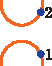
\includegraphics[scale=1]{CupCapDots.pdf}}}}}

\newcommand{\dbeta}{\mathord{\vcenter{\hbox{
\includegraphics[scale=1]{dbeta.pdf}}}}}
\newcommand{\dpsi}{\mathord{\vcenter{\hbox{
\includegraphics[scale=1]{dpsi.pdf}}}}}
\newcommand{\dblank}{\mathord{\vcenter{\hbox{
\includegraphics[scale=1]{dblank.pdf}}}}}





\newcommand{\SigmaDotDot}{\mathord{\vcenter{\hbox{
\includegraphics[scale=1]{SigmaDotDot.pdf}}}}}
\newcommand{\SigmaDotDotExchange}{\mathord{\vcenter{\hbox{
\includegraphics[scale=1]{SigmaDotDotExchange.pdf}}}}}
\newcommand{\TwoLine}{\mathord{\vcenter{\hbox{
\includegraphics[scale=1]{TwoLine.pdf}}}}}
\newcommand{\TwoLineDots}{\mathord{\vcenter{\hbox{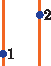
\includegraphics[scale=1]{TwoLineDots.pdf}}}}}


\newcommand{\RDotTwo}{\mathord{\vcenter{\hbox{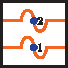
\includegraphics[scale=1]{RDotTwo.pdf}}}}}
\newcommand{\RDotTwoa}{\mathord{\vcenter{\hbox{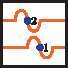
\includegraphics[scale=1]{RDotTwoa.pdf}}}}}
\newcommand{\RDotTwob}{\mathord{\vcenter{\hbox{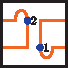
\includegraphics[scale=1]{RDotTwob.pdf}}}}}
\newcommand{\RDotTwoc}{\mathord{\vcenter{\hbox{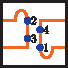
\includegraphics[scale=1]{RDotTwoc.pdf}}}}}

\newcommand{\FubeXXX}{\mathord{\vcenter{\hbox{
\includegraphics[scale=1]{EmptyTube.pdf}}}}}
\newcommand{\FubeXss}{\mathord{\vcenter{\hbox{
\includegraphics[scale=1]{OneLine.pdf}}}}}
\newcommand{\FubeXsds}{\mathord{\vcenter{\hbox{
\includegraphics[scale=1]{OneLineDot.pdf}}}}}



\newcommand{\AnnulusCut}{\mathord{\vcenter{\hbox{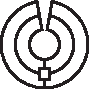
\includegraphics[scale=1]{AnnulusCut.pdf}}}}}
\newcommand{\AnnulusFlat}{\mathord{\vcenter{\hbox{
\includegraphics[scale=1]{AnnulusFlat.pdf}}}}}
\newcommand{\Disc}{\mathord{\vcenter{\hbox{
\includegraphics[scale=1]{Disc.pdf}}}}}
\newcommand{\RotatedTube}{\mathord{\vcenter{\hbox{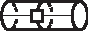
\includegraphics[scale=1]{RotatedTube.pdf}}}}}
\newcommand{\AnnulusGeneric}{\mathord{\vcenter{\hbox{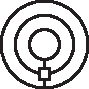
\includegraphics[scale=1]{AnnulusGeneric.pdf}}}}}



\newcommand{\FubeXXXA}{\mathord{\vcenter{\hbox{
\includegraphics[scale=1]{EmptyTubeA.pdf}}}}}
\newcommand{\FubeXssA}{\mathord{\vcenter{\hbox{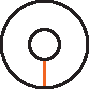
\includegraphics[scale=1]{OneLineA.pdf}}}}}
\newcommand{\FubeXsdsA}{\mathord{\vcenter{\hbox{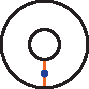
\includegraphics[scale=1]{OneLineDotA.pdf}}}}}

\newcommand{\FubesddXsA}{\mathord{\vcenter{\hbox{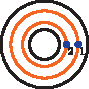
\includegraphics[scale=1]{FubesddXsA.pdf}}}}}

\newcommand{\RDotTwobA}{\mathord{\vcenter{\hbox{
\includegraphics[scale=1]{RDotTwobA.pdf}}}}}\newcommand{\RDotTwocA}{\mathord{\vcenter{\hbox{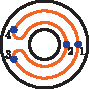
\includegraphics[scale=1]{RDotTwocA.pdf}}}}}


 
\newcommand{\Fubex}[2]{{\mathord{\ooalign{ \vphantom{$\Big|^2$}\cr\hidewidth\ensuremath{\scriptstyle{#2}}\hidewidth\cr$\vcenter{\hbox{$#1$}}$\cr
  \hidewidth\raise0ex\hbox{$\scale{1.2}{\VerticalSpace}$}\cr
  }}}}	




\newcommand{\TubeBC}{\mathord{\vcenter{\hbox{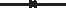
\includegraphics[scale=1]{TubeBC.pdf}}}}}

\newcommand{\TubeBCx}[1]{{\mathord{\ooalign{ \vphantom{$\Big|^2$}\cr\hidewidth\ensuremath{\scriptstyle{#1}}\hidewidth\cr$\vcenter{\hbox{$\scale{1}{\TubeBC}$}}$\cr
  \hidewidth\raise0ex\hbox{$\scale{.25}{\VerticalSpace}$}\cr
  }}}}	

\newcommand{\AnnulusBare}{\mathord{\vcenter{\hbox{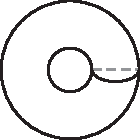
\includegraphics[scale=.6]{AnnulusBare.pdf}}}}}
\newcommand{\AnnularTube}{\mathord{\vcenter{\hbox{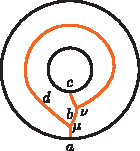
\includegraphics[scale=1]{AnnularTube.pdf}}}}}
\newcommand{\AnnularTubeNoIndex}{\mathord{\vcenter{\hbox{
\includegraphics[scale=1]{AnnularTubeNoIndex.pdf}}}}}
\newcommand{\AnnulusTubeTube}{\mathord{\vcenter{\hbox{
\includegraphics[scale=1]{AnnulusTubeTube.pdf}}}}}

\newcommand{\SAnnulusNoLabel}{\mathord{\vcenter{\hbox{
\includegraphics[scale=1]{SAnnulusNoLabel.pdf}}}}}
\newcommand{\TAnnulusNoLabel}{\mathord{\vcenter{\hbox{
\includegraphics[scale=1]{TAnnulusNoLabel.pdf}}}}}


\newcommand{\EdgeTensor}{\mathord{\vcenter{\hbox{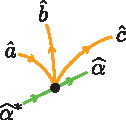
\includegraphics[scale=1]{EdgeTensor.pdf}}}}}

\newcommand{\OneHandleTheta}{\mathord{\vcenter{\hbox{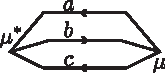
\includegraphics[scale=.7]{OneHandleTheta.pdf}}}}}
\newcommand{\OneHandlemud}{\mathord{\vcenter{\hbox{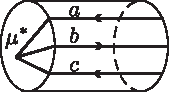
\includegraphics[scale=.7]{OneHandlemud.pdf}}}}}
\newcommand{\OneHandlemu}{\mathord{\vcenter{\hbox{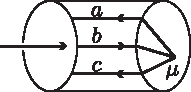
\includegraphics[scale=.7]{OneHandlemu.pdf}}}}}
\newcommand{\OneHandlea}{\mathord{\vcenter{\hbox{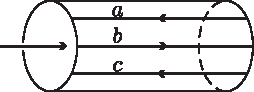
\includegraphics[scale=.7]{OneHandlea.pdf}}}}}

\newcommand{\Tetrahedron}{\mathord{\vcenter{\hbox{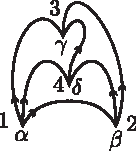
\includegraphics[scale=1]{Tetrahedron.pdf}}}}}
\newcommand{\PitchforkIdempotent}{\mathord{\vcenter{\hbox{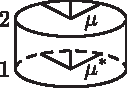
\includegraphics[scale=0.7]{PitchforkIdempotent.pdf}}}}}

\newcommand{\Pitchforkabc}{\mathord{\vcenter{\hbox{\includegraphics[scale=1]{Pitchforkabc.pdf}}}}}
\newcommand{\Pitchforkabcrot}{\mathord{\vcenter{\hbox{\includegraphics[scale=1]{Pitchforkabcrot.pdf}}}}}






\newcommand{\AnnulsLabel}[5]{\mathord{ 
\mkern2mu\overset{#3}{{\Annulusxprime{#1}{#2}}}\mkern2mu\raisebox{0ex}{$\scriptstyle{#4}$} }}

\newcommand*{\Annulus}[2]{{ #1 }
\kern-3.5em\raisebox{1ex}{ $\scriptstyle{#2}$} \kern2.6em} %Could change 0 to 1.2 to raise the B.

\newcommand*{\AnnulusP}[3]{{{\Annulus{#1}{#2}} }
\kern-.5em\raisebox{3.5ex}{ $\scriptstyle{#3}$} \kern.3em} %Could change 0 to 1.2 to raise the B.

\newcommand*{\AnnulusPx}[4]{\AnnulusP{#1}{#2}{#3}
\kern-3.6em\raisebox{-4.5ex}{ $\scriptstyle{#4}$} \kern2.6em} %Could change 0 to 1.2 to raise the B.

\newcommand*{\AnularTubex}[6]{\AnnulusPx{#1}{#2}{#3}{#4}
\kern-4em\raisebox{-4.5ex}{ $\overset{#6}{\underset{#5}{\vphantom{\Big|^2}}}$} \kern3em} %Could change 0 to 1.2 to raise the B.

\newcommand*{\TorusTubex}[6]{\AnnulusPx{#1}{#2}{#3}{#4}
\kern-4em\raisebox{-4.5ex}{ $\overset{#6}{\underset{#5}{\vphantom{\Big|^2}}}$} \kern3em} %Could change 0 to 1.2 to raise the B.

%\newcommand*{\AnnularTubex}[5]{\AnnulusPx{#1}{#2}{}{\; \; \;#3}
%\kern-3.9em\raisebox{-4.5ex}{ $\overset{#5}{\underset{#4}{\vphantom{\Big|^2}}}$} \kern2.7em} %Could change 0 to 1.2 to raise the B.



\newcommand{\SAnnulusx}[3]{\mathrel{\ooalign{$\SAnnulusNoLabel$\cr
  \hidewidth\raise5ex\hbox{$\scriptstyle{#3}\mkern1mu$}\cr
  \hidewidth\raise.8ex\hbox{$\scriptstyle{#2}\mkern63mu$}\cr
    \hidewidth\raise-3.8ex\hbox{$\scriptstyle{#1}\mkern39mu$}\cr
  }}}
  
  \newcommand{\TAnnulusx}[3]{\mathrel{\ooalign{$\TAnnulusNoLabel$\cr
  \hidewidth\raise5ex\hbox{$\scriptstyle{#3}\mkern1mu$}\cr
  \hidewidth\raise.8ex\hbox{$\scriptstyle{#2}\mkern63mu$}\cr
    \hidewidth\raise-4.9ex\hbox{$\scriptstyle{#1}\mkern51mu$}\cr
  }}}

\newcommand{\AnnularTubex}[6]{\mathrel{\ooalign{$#1$\cr
  \hidewidth\raise5ex\hbox{$\scriptstyle{#6}\mkern1mu$}\cr
  \hidewidth\raise.8ex\hbox{$\scriptstyle{#5}\mkern63mu$}\cr
  \hidewidth\raise-.9ex\hbox{$\scriptstyle{#3}\mkern68mu$}\cr
    \hidewidth\raise-4.5ex\hbox{$\scriptstyle{#4} \mkern50mu$}\cr
  \hidewidth\raise-7ex\hbox{$\scriptstyle{#2}\mkern68mu$}\cr
  }}}
  
%\newcommand{\AnnularTubexp}[9]{\mathrel{\ooalign{$#1$\cr
  %\hidewidth\raise5ex\hbox{$\scriptstyle{#9}\mkern1mu$}\cr
 %\hidewidth\raise.8ex\hbox{$\scriptstyle{#8}\mkern63mu$}\cr
 % \hidewidth\raise-3.4ex\hbox{$\scriptstyle{#7}\mkern68mu$}\cr
  %  \hidewidth\raise-5.1ex\hbox{$\scriptstyle{#6}\mkern80mu$}\cr
%  \hidewidth\raise-2.2ex\hbox{$\scriptstyle{#5}\mkern90mu$}\cr
 % \hidewidth\raise-.9ex\hbox{$\scriptstyle{#4}\mkern68mu$}\cr
%    \hidewidth\raise-4.5ex\hbox{$\scriptstyle{#3} \mkern50mu$}\cr
 % \hidewidth\raise-7ex\hbox{$\scriptstyle{#2}\mkern68mu$}\cr
 % }}}



\newcommand{\AnnularTubexp}[9]{\mathrel{\ooalign{$#1$\cr
  \hidewidth\raise5ex\hbox{$\scriptstyle{#9}\mkern1mu$}\cr
 \hidewidth\raise.8ex\hbox{$\scriptstyle{#8}\mkern63mu$}\cr
  \hidewidth\raise-3.7ex\hbox{$\scriptstyle{#7}\mkern50mu$}\cr
    \hidewidth\raise-5.1ex\hbox{$\scriptstyle{#6}\mkern57mu$}\cr
  \hidewidth\raise-2.2ex\hbox{$\scriptstyle{#5}\mkern90mu$}\cr
  \hidewidth\raise-.9ex\hbox{$\scriptstyle{#4}\mkern68mu$}\cr
    \hidewidth\raise-3.8ex\hbox{$\scriptstyle{#3} \mkern69mu$}\cr
  \hidewidth\raise-7ex\hbox{$\scriptstyle{#2}\mkern68mu$}\cr
  }}}


\newcommand{\SmallTorus}[3]{\mathrel{\ooalign{$#1$\cr
  \hidewidth\raise0ex\hbox{$\scriptstyle{#2}\mkern36mu$}\cr
    \hidewidth\raise-1.5ex\hbox{$\scriptstyle{#3}\mkern10mu$}\cr
  }}}
  
  
  \newcommand{\AnnulusTubeTubex}[6]{\mathrel{\ooalign{$#1$\cr
%  \hidewidth\raise5ex\hbox{$\scriptstyle{#7}\mkern1mu$}\cr
  \hidewidth\raise.8ex\hbox{$\scriptstyle{#6}\mkern65mu$}\cr
  \hidewidth\raise-.5ex\hbox{$\scriptstyle{#3}\mkern68mu$}\cr
    \hidewidth\raise-4.9ex\hbox{$\scriptstyle{#4} \mkern50mu$}\cr
     \hidewidth\raise-2.7ex\hbox{$\scriptstyle{#5} \mkern54mu$}\cr
  \hidewidth\raise-7.3ex\hbox{$\scriptstyle{#2}\mkern68mu$}\cr
  }}}
  

  \newcommand{\Cellup}{\mathord{\vcenter{\hbox{\includegraphics[scale=1]{Cellup.pdf}}}}}
    \newcommand{\Celldown}{\mathord{\vcenter{\hbox{\includegraphics[scale=1]{Celldown.pdf}}}}}
        \newcommand{\Cellmid}{\mathord{\vcenter{\hbox{\includegraphics[scale=1]{Cellmid.pdf}}}}}
        \newcommand{\TwoCell}{\mathord{\vcenter{\hbox{\includegraphics[scale=1]{TwoCell.pdf}}}}}
                \newcommand{\Onecell}{\mathord{\vcenter{\hbox{\includegraphics[scale=1]{Onecell.pdf}}}}}      
        
        

 


\newcommand{\TorusLocalRelationc}{\mathord{\vcenter{\hbox{\includegraphics[scale=1]{TorusLocalRelationc.pdf}}}}}
\newcommand{\TorusLocalRelationb}{\mathord{\vcenter{\hbox{\includegraphics[scale=1]{TorusLocalRelationb.pdf}}}}}
\newcommand{\TorusLocalRelationa}{\mathord{\vcenter{\hbox{\includegraphics[scale=1]{TorusLocalRelationa.pdf}}}}}


\newcommand{\Dv}{\mathord{\vcenter{\hbox{\includegraphics[scale=1]{Dv.pdf}}}}}
\newcommand{\Dfv}{\mathord{\vcenter{\hbox{\includegraphics[scale=1]{Dfv.pdf}}}}}


\newcommand{\Horseshoe}{\mathord{\vcenter{\hbox{\includegraphics[scale=1]{Horseshoe.pdf}}}}}
\newcommand{\HorseshoeTwist}{\mathord{\vcenter{\hbox{\includegraphics[scale=1]{HorseshoeTwist.pdf}}}}}
\newcommand{\euv}{\mathord{\vcenter{\hbox{\includegraphics[scale=1]{euv.pdf}}}}}
\newcommand{\chieuv}{\mathord{\vcenter{\hbox{\includegraphics[scale=1]{chieuv.pdf}}}}}


\newcommand{\TubeElement}{\mathord{\vcenter{\hbox{\includegraphics[scale=1]{TubeElement.pdf}}}}}


\newcommand{\LoopOverId}{\mathord{\vcenter{\hbox{\includegraphics[scale=1]{LoopOverId.pdf}}}}}
\newcommand{\Ida}{\mathord{\vcenter{\hbox{\includegraphics[scale=1]{Ida.pdf}}}}}
\newcommand{\OmegaSLoop}{\mathord{\vcenter{\hbox{\includegraphics[scale=1]{OmegaSLoop.pdf}}}}}

\newcommand{\IdxOmegaLoopa}{\mathord{\vcenter{\hbox{\includegraphics[scale=1]{IdxOmegaLoopa.pdf}}}}}
\newcommand{\IdxOmegaLoopb}{\mathord{\vcenter{\hbox{\includegraphics[scale=1]{IdxOmegaLoopb.pdf}}}}}


\newcommand{\HandleSlidea}{\mathord{\vcenter{\hbox{\includegraphics[scale=1]{HandleSlidea.pdf}}}}}
\newcommand{\HandleSlideb}{\mathord{\vcenter{\hbox{\includegraphics[scale=1]{HandleSlideb.pdf}}}}}


\newcommand{\TubeBasisa}{\mathord{\vcenter{\hbox{\includegraphics[scale=1]{TubeBasisa.pdf}}}}}
\newcommand{\TubeBasisb}{\mathord{\vcenter{\hbox{\includegraphics[scale=1]{TubeBasisb.pdf}}}}}
\newcommand{\TubeBasisc}{\mathord{\vcenter{\hbox{\includegraphics[scale=1]{TubeBasisc.pdf}}}}}
\newcommand{\TubeBasisd}{\mathord{\vcenter{\hbox{\includegraphics[scale=1]{TubeBasisd.pdf}}}}}
\newcommand{\TubeBasisdprime}{\mathord{\vcenter{\hbox{\includegraphics[scale=1]{TubeBasisdprime.pdf}}}}}


\newcommand{\gxyaj}{\mathord{\vcenter{\hbox{\includegraphics[scale=1]{gxyaj.pdf}}}}}
\newcommand{\hxyai}{\mathord{\vcenter{\hbox{\includegraphics[scale=1]{hxyai.pdf}}}}}

\newcommand{\VxyaoVxya}{\mathord{\vcenter{\hbox{\includegraphics[scale=1]{VxyaoVxya.pdf}}}}}
\newcommand{\idaprime}{\mathord{\vcenter{\hbox{\includegraphics[scale=1]{idaprime.pdf}}}}}

\newcommand{\Vxyxy}{\mathord{\vcenter{\hbox{\includegraphics[scale=1]{Vxyxy.pdf}}}}}
\newcommand{\idxy}{\mathord{\vcenter{\hbox{\includegraphics[scale=1]{idxy.pdf}}}}}
\newcommand{\Vxyxyomega}{\mathord{\vcenter{\hbox{\includegraphics[scale=1]{Vxyxyomega.pdf}}}}}



\newcommand{\SpinStructureProjector}{\mathord{\vcenter{\hbox{\includegraphics[scale=1]{SpinStructureProjector.pdf}}}}}


\newcommand{\EmptyTubeW}{\mathord{\vcenter{\hbox{\includegraphics[scale=1]{EmptyTubeW.pdf}}}}}

\newcommand{\TubeProject}{\mathord{\vcenter{\hbox{\includegraphics[scale=1]{TubeProject.pdf}}}}}


\newcommand{\TuberraJ}{\mathord{\vcenter{\hbox{\includegraphics[scale=1]{TuberraJ.pdf}}}}}
\newcommand{\Tubeidr}{\mathord{\vcenter{\hbox{\includegraphics[scale=1]{Tubeidr.pdf}}}}}
\newcommand{\Tuberr}{\mathord{\vcenter{\hbox{\includegraphics[scale=1]{Tuberr.pdf}}}}}


\newcommand{\TuberrTraceCe}{\mathord{\vcenter{\hbox{\includegraphics[scale=1]{TuberrTraceCe.pdf}}}}}
\newcommand{\TuberrTraceCo}{\mathord{\vcenter{\hbox{\includegraphics[scale=1]{TuberrTraceCo.pdf}}}}}



\newcommand{\exyomegaa}{\mathord{\vcenter{\hbox{\includegraphics[scale=1]{exyomegaa.pdf}}}}}
\newcommand{\exyomegab}{\mathord{\vcenter{\hbox{\includegraphics[scale=1]{exyomegab.pdf}}}}}
\newcommand{\exyomegac}{\mathord{\vcenter{\hbox{\includegraphics[scale=1]{exyomegac.pdf}}}}}

\newcommand{\EFunctora}{\mathord{\vcenter{\hbox{\includegraphics[scale=1]{EFunctora.pdf}}}}}
\newcommand{\EFunctorb}{\mathord{\vcenter{\hbox{\includegraphics[scale=1]{EFunctorb.pdf}}}}}
\newcommand{\EFunctorc}{\mathord{\vcenter{\hbox{\includegraphics[scale=1]{EFunctorc.pdf}}}}}



\newcommand{\TubeIdempotentTwoStrand}{\mathord{\vcenter{\hbox{\includegraphics[scale=1]{TubeIdempotentTwoStrand.pdf}}}}}
\newcommand{\fTubeCf}{\mathord{\vcenter{\hbox{\includegraphics[scale=1]{fTubeCf.pdf}}}}}
\newcommand{\fTubefOdd}{\mathord{\vcenter{\hbox{\includegraphics[scale=1]{fTubefOdd.pdf}}}}}
\newcommand{\minimalBosonic}{\mathord{\vcenter{\hbox{\includegraphics[scale=1]{minimalBosonic.pdf}}}}}



\newcommand{\FusionIsomorphism}{\mathord{\vcenter{\hbox{\includegraphics[scale=1]{FusionIsomorphism.pdf}}}}}


\newcommand{\TubeCompletea}{\mathord{\vcenter{\hbox{\includegraphics[scale=1]{TubeCompletea.pdf}}}}}
\newcommand{\TubeCompleteb}{\mathord{\vcenter{\hbox{\includegraphics[scale=1]{TubeCompleteb.pdf}}}}}
\newcommand{\TubeCompletec}{\mathord{\vcenter{\hbox{\includegraphics[scale=1]{TubeCompletec.pdf}}}}}
\newcommand{\TubeCompletecprime}{\mathord{\vcenter{\hbox{\includegraphics[scale=1]{TubeCompletecprime.pdf}}}}}



\newcommand{\Ufghk}{\mathord{\vcenter{\hbox{\includegraphics[scale=1]{Ufghk.pdf}}}}}


\newcommand{\fxyaJ}{\mathord{\vcenter{\hbox{\includegraphics[scale=1]{fxyaJ.pdf}}}}}


\newcommand{\TubeTwotoOneStrand}{\mathord{\vcenter{\hbox{\includegraphics[scale=1]{TubeTwotoOneStrand.pdf}}}}}
\newcommand{\TubeOnetoTwoStrand}{\mathord{\vcenter{\hbox{\includegraphics[scale=1]{TubeOnetoTwoStrand.pdf}}}}}
 

\newcommand{\SMatrix}[2]{\mathrel{\ooalign{$\OmegaSLoop$\cr
  \hidewidth\raise0ex\hbox{$\scriptstyle{#1}\mkern18mu$}\cr
    \hidewidth\raise0ex\hbox{$\scriptstyle{#2}\mkern-10mu$}\cr
  }}}
  
  
  \newcommand{\SMatrixx}[2]{\mathrel{\ooalign{$\OmegaSLoop$\cr
  \hidewidth\raise0ex\hbox{$\scriptstyle{#1}\mkern12mu$}\cr
    \hidewidth\raise0ex\hbox{$\scriptstyle{#2}\mkern-10mu$}\cr
  }}}
  
  \newcommand{\OmegaLoopDefectx}[2]{\mathrel{\ooalign{$\OmegaLoopDefect$\cr
  \hidewidth\raise0ex\hbox{$\scriptstyle{#1}\mkern8mu$}\cr
    \hidewidth\raise0ex\hbox{$\scriptstyle{#2}\mkern-22mu$}\cr
  }}}
  
  \newcommand{\OmegaLoopDefect}{\mathord{\vcenter{\hbox{\includegraphics[scale=1]{OmegaLoopDefect.pdf}}}}}
    \newcommand{\DiscGray}{\mathord{\vcenter{\hbox{\includegraphics[scale=1]{DiscGray.pdf}}}}}
    
    
    
\newcommand{\DCSmatrixf}{\mathord{\vcenter{\hbox{\includegraphics[scale=1]{DCSmatrixf.pdf}}}}}
\newcommand{\DCSmatrixa}{\mathord{\vcenter{\hbox{\includegraphics[scale=1]{DCSmatrixa.pdf}}}}}
\newcommand{\DCSmatrixb}{\mathord{\vcenter{\hbox{\includegraphics[scale=1]{DCSmatrixb.pdf}}}}}\newcommand{\DCSmatrixc}{\mathord{\vcenter{\hbox{\includegraphics[scale=1]{DCSmatrixc.pdf}}}}}
\newcommand{\DCSmatrixd}{\mathord{\vcenter{\hbox{\includegraphics[scale=1]{DCSmatrixd.pdf}}}}}
\newcommand{\DCSmatrixe}{\mathord{\vcenter{\hbox{\includegraphics[scale=1]{DCSmatrixe.pdf}}}}}

\newcommand{\DCSmatrixg}{\mathord{\vcenter{\hbox{\includegraphics[scale=1]{DCSmatrixg.pdf}}}}}
\newcommand{\DCSmatrixh}{\mathord{\vcenter{\hbox{\includegraphics[scale=1]{DCSmatrixh.pdf}}}}}


\newcommand{\STorusBasisa}{\mathord{\vcenter{\hbox{\includegraphics[scale=1]{STorusBasisa.pdf}}}}}


\newcommand{\Scalcae}{\mathord{\vcenter{\hbox{\includegraphics[scale=1]{Scalcae.pdf}}}}}  
\newcommand{\Scalcad}{\mathord{\vcenter{\hbox{\includegraphics[scale=1]{Scalcad.pdf}}}}}  
\newcommand{\Scalcac}{\mathord{\vcenter{\hbox{\includegraphics[scale=1]{Scalcac.pdf}}}}}  
\newcommand{\Scalcab}{\mathord{\vcenter{\hbox{\includegraphics[scale=1]{Scalcab.pdf}}}}}
\newcommand{\Scalcaa}{\mathord{\vcenter{\hbox{\includegraphics[scale=1]{Scalcaa.pdf}}}}}  


\newcommand{\Scalcbe}{\mathord{\vcenter{\hbox{\includegraphics[scale=1]{Scalcbe.pdf}}}}}  
\newcommand{\Scalcbd}{\mathord{\vcenter{\hbox{\includegraphics[scale=1]{Scalcbd.pdf}}}}}  
\newcommand{\Scalcbc}{\mathord{\vcenter{\hbox{\includegraphics[scale=1]{Scalcbc.pdf}}}}}  
\newcommand{\Scalcbb}{\mathord{\vcenter{\hbox{\includegraphics[scale=1]{Scalcbb.pdf}}}}}
\newcommand{\Scalcba}{\mathord{\vcenter{\hbox{\includegraphics[scale=1]{Scalcba.pdf}}}}}  


\newcommand{\Scalcbedot}{\mathord{\vcenter{\hbox{\includegraphics[scale=1]{Scalcbedot.pdf}}}}}  
\newcommand{\Scalcbddot}{\mathord{\vcenter{\hbox{\includegraphics[scale=1]{Scalcbddot.pdf}}}}}  
\newcommand{\Scalcbadot}{\mathord{\vcenter{\hbox{\includegraphics[scale=1]{Scalcbadot.pdf}}}}}    
  

  
%\newcommand{\SMatrix}[2]{\mathrel{\ooalign{$\OmegaSLoop$
%\mathrel{\raisebox{#1}{$\oldsqsubset$}}
  %\hidewidth\raise0ex\hbox{$\scriptstyle{a}\mkern0mu$}\cr
    %\hidewidth\raise0ex\hbox{$\scriptstyle{b}\mkern0mu$}\cr
%    \hidewidth\raise-4.3ex\hbox{$\scriptstyle{#2}\mkern43mu$}\cr
%        \hidewidth\raise-6.3ex\hbox{$\scriptstyle{#2}\mkern61mu$}\cr
%        \hidewidth\raise4.1ex\hbox{$\scriptstyle{#4}\mkern25mu$}\cr
  %              \hidewidth\raise-0.3ex\hbox{$\scriptstyle{#3}\mkern60mu$}\cr
%          \hidewidth\raise0ex\hbox{$\scale{1.5}{\VerticalSpace}$}\cr
 %}}}
 
 
\newcommand{\LoopArrow}{\mathord{\vcenter{\hbox{\includegraphics[scale=1]{LoopArrow.pdf}}}}}  
\newcommand{\LoopArrowx}[1]{\mathrel{\ooalign{$\LoopArrow_{\mathrel{\raisebox{4pt}{$\scriptstyle{#1}$}}}$
  }}}
  
  
\newcommand{\OmegaLoop}{\mathord{\vcenter{\hbox{\includegraphics[scale=1]{OmegaLoop.pdf}}}}}  
\newcommand{\OmegaLoopx}[1]{\mathrel{\ooalign{$\OmegaLoop_{\mathrel{\raisebox{4pt}{$\scriptstyle{#1}$}}}$
  }}}



\newcommand{\TubeElementx}[3]{\mathrel{\ooalign{$\TubeElement$\cr
  \hidewidth\raise-3.55ex\hbox{$\scriptstyle{#1}\mkern62mu$}\cr
%    \hidewidth\raise-4.3ex\hbox{$\scriptstyle{#2}\mkern43mu$}\cr
        \hidewidth\raise-6.3ex\hbox{$\scriptstyle{#2}\mkern61mu$}\cr
%        \hidewidth\raise4.1ex\hbox{$\scriptstyle{#4}\mkern25mu$}\cr
                \hidewidth\raise-0.3ex\hbox{$\scriptstyle{#3}\mkern60mu$}\cr
          \hidewidth\raise0ex\hbox{$\scale{1.5}{\VerticalSpace}$}\cr
  }}}

\newcommand{\IdempotentMTCNoLabel}{\mathord{\vcenter{\hbox{\includegraphics[scale=1]{IdempotentMTC.pdf}}}}}
\newcommand{\IdempBraid}[5]{\mathrel{\ooalign{$\IdempotentMTCNoLabel$\cr
  \hidewidth\raise-4.3ex\hbox{$\scriptstyle{#1}\mkern78mu$}\cr
    \hidewidth\raise-4.3ex\hbox{$\scriptstyle{#2}\mkern43mu$}\cr
        \hidewidth\raise-6.3ex\hbox{$\scriptstyle{#3}\mkern61mu$}\cr
        \hidewidth\raise4.1ex\hbox{$\scriptstyle{#4}\mkern25mu$}\cr
                \hidewidth\raise0ex\hbox{$\scriptstyle{#5}\mkern60mu$}\cr
          \hidewidth\raise0ex\hbox{$\scale{1.5}{\VerticalSpace}$}\cr
  }}}
  
\newcommand{\TorusBasisMTCNoLabel}{\mathord{\vcenter{\hbox{\includegraphics[scale=1]{TorusBasisMTC.pdf}}}}}
\newcommand{\TorusBraidBasis}[6]{\mathrel{\ooalign{$\TorusBasisMTCNoLabel$\cr
  \hidewidth\raise-4.3ex\hbox{$\scriptstyle{#1}\mkern78mu$}\cr
    \hidewidth\raise-4.3ex\hbox{$\scriptstyle{#2}\mkern40mu$}\cr
        \hidewidth\raise-6.3ex\hbox{$\scriptstyle{#3}\mkern61mu$}\cr
        \hidewidth\raise4.1ex\hbox{$\scriptstyle{#4}\mkern25mu$}\cr
                \hidewidth\raise0ex\hbox{$\scriptstyle{#5}\mkern58mu$}\cr
                                \hidewidth\raise4.7ex\hbox{$\scriptstyle{#6}\mkern0mu$}\cr
          \hidewidth\raise0ex\hbox{$\scale{1.5}{\VerticalSpace}$}\cr
  }}}
  
  \newcommand{\tcca}{\mathord{\vcenter{\hbox{\includegraphics[scale=1]{tcca.pdf}}}}}
    \newcommand{\tccb}{\mathord{\vcenter{\hbox{\includegraphics[scale=1]{tccb.pdf}}}}}
     \newcommand{\tccc}{\mathord{\vcenter{\hbox{\includegraphics[scale=1]{tccc.pdf}}}}}
      \newcommand{\tccd}{\mathord{\vcenter{\hbox{\includegraphics[scale=1]{tccd.pdf}}}}}
   
  
 


\newcommand{\TorusBasisMTCdl}{\mathord{\vcenter{\hbox{\includegraphics[scale=1]{TorusBasisMTCdl.pdf}}}}}
\newcommand{\TorusBasisMTCdr}{\mathord{\vcenter{\hbox{\includegraphics[scale=1]{TorusBasisMTCdr.pdf}}}}}
\newcommand{\TorusBasisMTCdd}{\mathord{\vcenter{\hbox{\includegraphics[scale=1]{TorusBasisMTCdd.pdf}}}}}
 
 \newcommand{\TorusBraidBasisd}[7]{\mathrel{\ooalign{$#7$\cr
  \hidewidth\raise-4.3ex\hbox{$\scriptstyle{#1}\mkern78mu$}\cr
    \hidewidth\raise-4.3ex\hbox{$\scriptstyle{#2}\mkern40mu$}\cr
        \hidewidth\raise-6.3ex\hbox{$\scriptstyle{#3}\mkern61mu$}\cr
        \hidewidth\raise4.1ex\hbox{$\scriptstyle{#4}\mkern25mu$}\cr
                \hidewidth\raise0ex\hbox{$\scriptstyle{#5}\mkern58mu$}\cr
                                \hidewidth\raise4.7ex\hbox{$\scriptstyle{#6}\mkern0mu$}\cr
          \hidewidth\raise0ex\hbox{$\scale{1.5}{\VerticalSpace}$}\cr
  }}}



\newcommand{\TaddownTubeNoLabel}{\mathord{\vcenter{\hbox{\includegraphics[scale=1]{TaddownTube.pdf}}}}}
\newcommand{\TadupTubeNoLabel}{\mathord{\vcenter{\hbox{\includegraphics[scale=1]{TadupTube.pdf}}}}}
\newcommand{\hTube}{\mathord{\vcenter{\hbox{\includegraphics[scale=1]{hTube.pdf}}}}}
\newcommand{\tTube}{\mathord{\vcenter{\hbox{\includegraphics[scale=1]{tTube.pdf}}}}}
\newcommand{\eTube}{\mathord{\vcenter{\hbox{\includegraphics[scale=1]{eTube.pdf}}}}}
\newcommand{\vTube}{\mathord{\vcenter{\hbox{\includegraphics[scale=1]{vTube.pdf}}}}}


\newcommand{\dota}{\mathord{\vcenter{\hbox{\includegraphics[scale=1]{dota.pdf}}}}}
\newcommand{\dotb}{\mathord{\vcenter{\hbox{\includegraphics[scale=1]{dotb.pdf}}}}}
\newcommand{\dotc}{\mathord{\vcenter{\hbox{\includegraphics[scale=1]{dotc.pdf}}}}}

\newcommand{\XTubeNoLabel}{\mathord{\vcenter{\hbox{\includegraphics[scale=1]{XTube.pdf}}}}}
\newcommand{\XTube}[2]{\mathrel{\ooalign{$\XTubeNoLabel$\cr
  \hidewidth\raise-2.5ex\hbox{$\scriptstyle{#2}\mkern28mu$}\cr
    \hidewidth\raise-2.9ex\hbox{$\scriptstyle{#1}\mkern50mu$}\cr
  }}}


\newcommand{\TaddownTube}[1]{\mathrel{\ooalign{$\TaddownTubeNoLabel$\cr
    \hidewidth\raise-2.8ex\hbox{$\scriptstyle{#1}\mkern30mu$}\cr
  }}}
  \newcommand{\TadupTube}[1]{\mathrel{\ooalign{$\TadupTubeNoLabel$\cr
    \hidewidth\raise-2.6ex\hbox{$\scriptstyle{#1}\mkern30mu$}\cr
  }}}
  
  \newcommand{\TorusNoLabels}{\mathord{\vcenter{\hbox{\includegraphics[scale=1]{TorusNoLabels.pdf}}}}}
\newcommand{\TorusNoLabelsx}[1]{\mathrel{\ooalign{$\TorusNoLabels$\cr
    \hidewidth\raise-2.8ex\hbox{$\scriptstyle{#1}\mkern30mu$}\cr
  }}}

\newcommand{\VerticalSpace}{\mathord{\vcenter{\hbox{\includegraphics[scale=1]{VerticalSpace.pdf}}}}}

\newcommand{\AddDat}[3]{\mathrel{\ooalign{  $#1$\cr
  \hidewidth\raise0ex\hbox{$\scriptstyle{#2}\mkern38mu$}\cr
  \hidewidth\raise0ex\hbox{${#3}\mkern0mu$}\cr
  \hidewidth\raise0ex\hbox{$\VerticalSpace$}\cr
  }}}
  
  \newcommand{\AddDatTorus}[3]{\mathrel{\ooalign{  $#1$\cr
  \hidewidth\raise0ex\hbox{$\scriptstyle{#2}\mkern38mu$}\cr
  \hidewidth\raise3.8ex\hbox{$\scriptstyle{#3}\mkern0mu$}\cr
  \hidewidth\raise0ex\hbox{$\VerticalSpace$}\cr
  }}}
  
    \newcommand{\AddDatTorusDot}[4]{\mathrel{\ooalign{  $#1$\cr
  \hidewidth\raise0ex\hbox{$\scriptstyle{#2}\mkern38mu$}\cr
  \hidewidth\raise3.8ex\hbox{$\scriptstyle{#3}\mkern0mu$}\cr
  \hidewidth\raise0ex\hbox{${#4}\mkern0mu$}\cr
  \hidewidth\raise0ex\hbox{$\VerticalSpace$}\cr
  }}}
  
  
  
 
  
   
  \newcommand{\TubeProductCoefficienta}{\mathord{\vcenter{\hbox{\includegraphics[scale=1]{TubeProductCoefficienta.pdf}}}}}
  \newcommand{\TubeProductCoefficientb}{\mathord{\vcenter{\hbox{\includegraphics[scale=1]{TubeProductCoefficientb.pdf}}}}}
  
    \newcommand{\ThetaSymbol}{\mathord{\vcenter{\hbox{\includegraphics[scale=1]{Theta.pdf}}}}}
 
   \newcommand{\ThetaSymbolx}[1]{\mathrel{\ooalign{$\ThetaSymbol$\cr
      \hidewidth\raise-1.3ex\hbox{$\scriptstyle{#1} \mkern0mu$}\cr
  }}}
  
  
    
  \newcommand{\TubeProductCoefficientbx}[2]{\mathrel{\ooalign{$\TubeProductCoefficientb \;\;\; $\cr
      \hidewidth\raise-.8ex\hbox{$\scriptstyle{#1} \mkern54mu$}\cr
      \hidewidth\raise-.8ex\hbox{$\scriptstyle{#2} \mkern6mu$}\cr
  }}}
  
  \newcommand{\TubeProductCoefficientax}[5]{\mathrel{\ooalign{$\TubeProductCoefficienta$\cr
      \hidewidth\raise-4.2ex\hbox{$\scriptstyle{#1} \mkern30mu$}\cr
      \hidewidth\raise-1.8ex\hbox{$\scriptstyle{#2} \mkern30mu$}\cr
  \hidewidth\raise6.1ex\hbox{$\scriptstyle{#3}\mkern44mu$}\cr
  \hidewidth\raise2.05ex\hbox{$\scriptstyle{#4}\mkern82mu$}\cr
    \hidewidth\raise3.2ex\hbox{$\scriptstyle{#5}\mkern3mu$}\cr
  }}}

  

  
    
\newcommand{\tubex}[8]{#1 \left(\substack{#8\\ \\ #5\\ } \; \substack{#4\\ #3\\ #2\\ }\; \substack{ #7 \\ #6} \right)}
%\newcommand*{\SmallTorus}[3]{\kern 2.05 em\raisebox{0ex}{ $\scriptstyle{#2}$} \kern-2.05em{ #1 } 
%\kern-1.1em\raisebox{-1.5ex}{$\scriptstyle{#3}$} \kern1.1em} %Could change 0 to 1.2 to raise the B.


%\newcommand*{\Tubex}[2]{{ \AnnularTube }
%\kern-3.5em\raisebox{1ex}{ $\scriptstyle{#2}$} \kern3.5em} %Could change 0 to 1.2 to raise the B.


%\newcommand{\BWfour}[5]{\mathord{ \raisebox{0.2ex}{$\scriptstyle{#2}$}\mkern2mu\overset{#3}{\underset{#4}{#1}}\mkern2mu\raisebox{0.2ex}{$\scriptstyle{#5}$} }}




\newcommand{\FubesXs}{\mathord{\vcenter{\hbox{\includegraphics[scale=1,angle=90,origin=c]{OneLine.pdf}}}}}
\newcommand{\FubesdXs}{\mathord{\vcenter{\hbox{\includegraphics[scale=1]{FubesdXs.pdf}}}}}

\newcommand{\FubessX}{\mathord{\vcenter{\hbox{\includegraphics[scale=1]{FubessX.pdf}}}}}
\newcommand{\FubessdX}{\mathord{\vcenter{\hbox{\includegraphics[scale=1]{FubessdX.pdf}}}}}

\newcommand{\FubesdXsA}{\mathord{\vcenter{\hbox{\includegraphics[scale=1]{FubesdXsA.pdf}}}}}
\newcommand{\FubessXA}{\mathord{\vcenter{\hbox{\includegraphics[scale=1]{FubessXA.pdf}}}}}
\newcommand{\FubessdXA}{\mathord{\vcenter{\hbox{\includegraphics[scale=1]{FubessdXA.pdf}}}}}


\newcommand{\FubesXsA}{\mathord{\vcenter{\hbox{\includegraphics[scale=1]{FubesXshA.pdf}}}}}
\newcommand{\FubesXsa}{\mathord{\vcenter{\hbox{\includegraphics[scale=1]{FubesXsa.pdf}}}}}
\newcommand{\FubesXsb}{\mathord{\vcenter{\hbox{\includegraphics[scale=1]{FubesXsb.pdf}}}}}
\newcommand{\FubesXsc}{\mathord{\vcenter{\hbox{\includegraphics[scale=1]{FubesXsc.pdf}}}}}


\newcommand{\FubesXscA}{\mathord{\vcenter{\hbox{\includegraphics[scale=1]{FubeXscA.pdf}}}}}
\newcommand{\FubesXsbA}{\mathord{\vcenter{\hbox{\includegraphics[scale=1]{FubeXsbA.pdf}}}}}
\newcommand{\FubesXsaA}{\mathord{\vcenter{\hbox{\includegraphics[scale=1]{FubeXsaA.pdf}}}}}






\newcommand{\qqo}{\mathord{\vcenter{\hbox{\includegraphics[scale=.4]{qq1.pdf}}}}}
\newcommand{\qtqo}{\mathord{\vcenter{\hbox{\includegraphics[scale=.4]{qtq1.pdf}}}}}
\newcommand{\qqto}{\mathord{\vcenter{\hbox{\includegraphics[scale=.4]{qqt1.pdf}}}}}
\newcommand{\qtqto}{\mathord{\vcenter{\hbox{\includegraphics[scale=.4]{qtqt1.pdf}}}}}
\newcommand{\qqm}{\mathord{\vcenter{\hbox{\includegraphics[scale=.4]{qqm.pdf}}}}}
\newcommand{\qtqm}{\mathord{\vcenter{\hbox{\includegraphics[scale=.4]{qtqm.pdf}}}}}
\newcommand{\qqtm}{\mathord{\vcenter{\hbox{\includegraphics[scale=.4]{qqtm.pdf}}}}}
\newcommand{\qtqtm}{\mathord{\vcenter{\hbox{\includegraphics[scale=.4]{qtqtm.pdf}}}}}

\newcommand{\PantsPAP}{\mathord{\vcenter{\hbox{\includegraphics[scale=0.7]{PantsPAP.pdf}}}}}
\newcommand{\PantsPAsP}{\mathord{\vcenter{\hbox{\includegraphics[scale=0.7]{PantsPAsP.pdf}}}}}

\newcommand{\PantsPsdAP}{\mathord{\vcenter{\hbox{\includegraphics[scale=0.7]{PantsPsdAP.pdf}}}}}
\newcommand{\PantsPsdAsP}{\mathord{\vcenter{\hbox{\includegraphics[scale=0.7]{PantsPsdAsP.pdf}}}}}



\newcommand{\PantsPPA}{\mathord{\vcenter{\hbox{\includegraphics[scale=0.7]{PantsPPA.pdf}}}}}
\newcommand{\PantsPPAs}{\mathord{\vcenter{\hbox{\includegraphics[scale=0.7]{PantsPPAs.pdf}}}}}

\newcommand{\PantsAsAshAsvt}{\mathord{\vcenter{\hbox{\includegraphics[scale=0.7]{PantsAsAshAsvt.pdf}}}}}
\newcommand{\PantsAstAAs}{\mathord{\vcenter{\hbox{\includegraphics[scale=0.7]{PantsAstAAs.pdf}}}}}

\newcommand{\PantsAstAshAs}{\mathord{\vcenter{\hbox{\includegraphics[scale=0.7]{PantsAstAshAs.pdf}}}}}
\newcommand{\PantsAsAshAs}{\mathord{\vcenter{\hbox{\includegraphics[scale=0.7]{PantsAsAshAs.pdf}}}}}
\newcommand{\PantsAsAAs}{\mathord{\vcenter{\hbox{\includegraphics[scale=0.7]{PantsAsAAs.pdf}}}}}

\newcommand{\Pantssvtsvtsh}{\mathord{\vcenter{\hbox{\includegraphics[scale=.7,origin=c]{Pantssvtsvtsh.pdf}}}}}
\newcommand{\Pantssvtsvsh}{\mathord{\vcenter{\hbox{\includegraphics[scale=.7,angle=0,origin=c]{Pantssvtsvsh.pdf}}}}}
\newcommand{\Pantssvsvtsh}{\mathord{\vcenter{\hbox{\includegraphics[scale=.7,angle=0,origin=c]{Pantssvsvtsh.pdf}}}}}
\newcommand{\Pantssvsvsh}{\mathord{\vcenter{\hbox{\includegraphics[scale=.7,angle=0,origin=c]{Pantssvsvsh.pdf}}}}}
\newcommand{\PantssvtsvtX}{\mathord{\vcenter{\hbox{\includegraphics[scale=.7,angle=0,origin=c]{PantssvtsvtX.pdf}}}}}
\newcommand{\PantssvtsvX}{\mathord{\vcenter{\hbox{\includegraphics[scale=.7,angle=0,origin=c]{PantssvtsvX.pdf}}}}}
%\newcommand{\PantssvtsvX}{\mathord{\vcenter{\hbox{\includegraphics[scale=.7,angle=0,origin=c]{PantssvtsvX.pdf}}}}}
\newcommand{\PantssvsvtX}{\mathord{\vcenter{\hbox{\includegraphics[scale=.7,angle=0,origin=c]{PantssvsvtX.pdf}}}}}
\newcommand{\PantssvsvX}{\mathord{\vcenter{\hbox{\includegraphics[scale=.7,angle=0,origin=c]{PantssvsvX.pdf}}}}}

\newcommand{\PantssvtXsvd}{\mathord{\vcenter{\hbox{\includegraphics[scale=.7,angle=0,origin=c]{PantssvtXsvd.pdf}}}}}
\newcommand{\Pantssvtshsvd}{\mathord{\vcenter{\hbox{\includegraphics[scale=.7,angle=0,origin=c]{Pantssvtshsvd.pdf}}}}}
\newcommand{\Pantssvshsvd}{\mathord{\vcenter{\hbox{\includegraphics[scale=.7,angle=0,origin=c]{Pantssvshsvd.pdf}}}}}
\newcommand{\PantssvXsvd}{\mathord{\vcenter{\hbox{\includegraphics[scale=.7,angle=0,origin=c]{PantssvXsvd.pdf}}}}}

\newcommand{\PantssvtXsvt}{\mathord{\vcenter{\hbox{\includegraphics[scale=.7,angle=0,origin=c]{PantssvtXsvt.pdf}}}}}
\newcommand{\PantssvXsvt}{\mathord{\vcenter{\hbox{\includegraphics[scale=.7,angle=0,origin=c]{PantssvXsvt.pdf}}}}}

\newcommand{\PantssvtXsv}{\mathord{\vcenter{\hbox{\includegraphics[scale=.7,angle=0,origin=c]{PantssvtXsv.pdf}}}}}



%%%%%%%%%%%%%%%%%%%%%%%%%%%%%%%%%%%%%%%%%%%%%%%%
%%%%%%%%%%%%%%%%%%%%%%%%%%%%%%%%%%%%%%%%%%%%%%%%
\newcommand{\PantssvXsvdA}{\mathord{\vcenter{\hbox{\includegraphics[scale=.8,angle=0,origin=c]{PantssvXsvdA.pdf}}}}}
\newcommand{\PantssvtXsvdA}{\mathord{\vcenter{\hbox{\includegraphics[scale=.8,angle=0,origin=c]{PantssvtXsvdA.pdf}}}}}
\newcommand{\PantssvtshsvdA}{\mathord{\vcenter{\hbox{\includegraphics[scale=.8,angle=0,origin=c]{PantssvtshsvdA.pdf}}}}}
\newcommand{\PantssvshsvdA}{\mathord{\vcenter{\hbox{\includegraphics[scale=.8,angle=0,origin=c]{PantssvshsvdA.pdf}}}}}
\newcommand{\PantsPsdAsPA}{\mathord{\vcenter{\hbox{\includegraphics[scale=.8,angle=0,origin=c]{PantsPsdAsPA.pdf}}}}}
\newcommand{\PantsPsdAPA}{\mathord{\vcenter{\hbox{\includegraphics[scale=.8,angle=0,origin=c]{PantsPsdAPA.pdf}}}}}
\newcommand{\PantsPPAsA}{\mathord{\vcenter{\hbox{\includegraphics[scale=.8,angle=0,origin=c]{PantsPPAsA.pdf}}}}}
\newcommand{\PantsPPAA}{\mathord{\vcenter{\hbox{\includegraphics[scale=.8,angle=0,origin=c]{PantsPPAA.pdf}}}}}
\newcommand{\PantsPAsPA}{\mathord{\vcenter{\hbox{\includegraphics[scale=.8,angle=0,origin=c]{PantsPAsPA.pdf}}}}}
\newcommand{\PantsPAPA}{\mathord{\vcenter{\hbox{\includegraphics[scale=.8,angle=0,origin=c]{PantsPAPA.pdf}}}}}
\newcommand{\PantsAstAAsA}{\mathord{\vcenter{\hbox{\includegraphics[scale=.8,angle=0,origin=c]{PantsAstAAsA.pdf}}}}}
\newcommand{\PantsAsAshAsvtA}{\mathord{\vcenter{\hbox{\includegraphics[scale=.8,angle=0,origin=c]{PantsAsAshAsvtA.pdf}}}}}
\newcommand{\PantsNNda}{\mathord{\vcenter{\hbox{\includegraphics[scale=.8,angle=0,origin=c]{PantsNNda.pdf}}}}}
\newcommand{\PantsNNd}{\mathord{\vcenter{\hbox{\includegraphics[scale=.8,angle=0,origin=c]{PantsNNd.pdf}}}}}
%%%%%%%%%%%%%%%%%%%%%%%%%%%%%%%%%%%%%%%%%%%%%%%%
%%%%%%%%%%%%%%%%%%%%%%%%%%%%%%%%%%%%%%%%%%%%%%%%

\newcommand{\TwoLinedotdot}{\mathord{\vcenter{\hbox{\includegraphics[scale=1.5,angle=0,origin=c]{TwoLinedotdot.pdf}}}}}

\newcommand{\Id}{\mathord{\vcenter{\hbox{\includegraphics[scale=1.5,angle=0,origin=c]{Id.pdf}}}}}

\newcommand{\CupSigmadot}{\mathord{\vcenter{\hbox{\includegraphics[scale=1.5,angle=0,origin=c]{Cupdot.pdf}}}}}

\newcommand{\CupSigma}{\mathord{\vcenter{\hbox{\includegraphics[scale=1.5,angle=0,origin=c]{Cup.pdf}}}}}

\newcommand{\StaggaredGSOdd}{\mathord{\vcenter{\hbox{\includegraphics[scale=1.5,angle=0,origin=c]{StaggaredGSOdd.pdf}}}}}
\newcommand{\StaggaredGSEven}{\mathord{\vcenter{\hbox{\includegraphics[scale=1.5,angle=0,origin=c]{StaggeredGSEven.pdf}}}}}

\newcommand{\StaggaredGSEvenR}{\mathord{\vcenter{\hbox{\reflectbox{\includegraphics[scale=1.5,angle=0,origin=c]{StaggeredGSEven.pdf}}}}}}





\newcommand{\VxsdsY}{\mathord{\vcenter{\hbox{\includegraphics[scale=0.3,angle=0,origin=c]{Vxsds.pdf}}}}}
\newcommand{\VsdxsY}{\mathord{\vcenter{\hbox{\includegraphics[scale=0.3,angle=0,origin=c]{Vsdxs.pdf}}}}}
\newcommand{\VtssdxY}{\mathord{\vcenter{\hbox{\includegraphics[scale=0.3,angle=0,origin=c]{Vtssdx.pdf}}}}}

\newcommand{\Vssdx}{\mathord{\vcenter{\hbox{\includegraphics[scale=0.3,angle=0,origin=c]{Vssdx.pdf}}}}}
\newcommand{\Vxsds}{\mathord{\vcenter{\hbox{\reflectbox{\includegraphics[scale=0.3,angle=0,origin=c]{Vssdx.pdf}}}}}}

\newcommand{\Vssx}{\mathord{\vcenter{\hbox{\includegraphics[scale=0.3,angle=0,origin=c]{Vssx.pdf}}}}}
\newcommand{\Vxss}{\mathord{\vcenter{\hbox{\reflectbox{\includegraphics[scale=0.3,angle=0,origin=c]{Vssx.pdf}}}}}}

\newcommand{\Vsxs}{\mathord{\vcenter{\hbox{\includegraphics[scale=0.3,angle=0,origin=c]{Vsxs.pdf}}}}}
\newcommand{\Vsxsd}{\mathord{\vcenter{\hbox{\includegraphics[scale=0.3,angle=0,origin=c]{Vsxsd.pdf}}}}}

\newcommand{\VsxsY}{\mathord{\vcenter{\hbox{\includegraphics[scale=0.3,angle=180,origin=c]{Vsxs.pdf}}}}}
\newcommand{\VssxY}{\mathord{\vcenter{\hbox{\includegraphics[scale=0.3,angle=180,origin=c]{Vssx.pdf}}}}}
\newcommand{\VxssY}{\mathord{\vcenter{\hbox{\reflectbox{\includegraphics[scale=0.3,angle=180,origin=c]{Vssx.pdf}}}}}}

\newcommand{\PsiFermion}{\mathord{\vcenter{\hbox{\includegraphics[scale=1.5]{PsiFermion.pdf}}}}}
\newcommand{\PsiFermionTwist}{\mathord{\vcenter{\hbox{\includegraphics[scale=1.5]{PsiFermionTwist.pdf}}}}}

\newcommand{\TwoFermion}{\mathord{\vcenter{\hbox{\includegraphics[scale=1.5]{TwoFermion.pdf}}}}}
\newcommand{\TwoFermionExchange}{\mathord{\vcenter{\hbox{\includegraphics[scale=1.5]{TwoFermionExchange.pdf}}}}}
\newcommand{\TwoFermionNoLabels}{\mathord{\vcenter{\hbox{\includegraphics[scale=1.5]{TwoFermion_nolabels.pdf}}}}}
\newcommand{\TwoFermionExchangeNoLabels}{\mathord{\vcenter{\hbox{\includegraphics[scale=1.5]{TwoFermionExchange_nolabels.pdf}}}}}


\newcommand{\Spin}{\mathord{\vcenter{\hbox{\includegraphics[scale=1.5]{Spin.pdf}}}}}
\newcommand{\PsiIdentity}{\mathord{\vcenter{\hbox{\includegraphics[scale=1.5]{PsiIdentity.pdf}}}}}

\newcommand{\TwoPsiExchange}{\mathord{\vcenter{\hbox{\includegraphics[scale=1.5]{TwoPsiExchange.pdf}}}}}
\newcommand{\TwoPsiIdentity}{\mathord{\vcenter{\hbox{\includegraphics[scale=1.5]{TwoPsiIdentity.pdf}}}}}


\newcommand{\PsiEnd}{\mathord{\vcenter{\hbox{\includegraphics[scale=1.5]{PsiEnd.pdf}}}}}
\newcommand{\PsiEndExchange}{\mathord{\vcenter{\hbox{\includegraphics[scale=1.5]{PsiEndExchange.pdf}}}}}

\newcommand{\DotSlidea}{\mathord{\vcenter{\hbox{\includegraphics[scale=1]{DotSlidea.pdf}}}}}
\newcommand{\DotSlideb}{\mathord{\vcenter{\hbox{\includegraphics[scale=1]{DotSlideb.pdf}}}}}
\newcommand{\DotSlidec}{\mathord{\vcenter{\hbox{\includegraphics[scale=1]{DotSlidec.pdf}}}}}
\newcommand{\DotSlided}{\mathord{\vcenter{\hbox{\includegraphics[scale=1]{DotSlided.pdf}}}}}

\newcommand{\QCapDotL}{\mathord{\vcenter{\hbox{\includegraphics[scale=1]{QDotslide.pdf}}}}}
\newcommand{\QCupDotR}{\mathord{\vcenter{\hbox{\includegraphics[scale=1,angle=180,origin=c]{QDotslide.pdf}}}}}
\newcommand{\QCapDotR}{\mathord{\vcenter{\hbox{\reflectbox{\includegraphics[scale=1]{QDotslide.pdf}}}}}}
\newcommand{\QCupDotL}{\mathord{\vcenter{\hbox{\reflectbox{\includegraphics[scale=1,angle=180,origin=c]{QDotslide.pdf}}}}}}

\newcommand{\TwodotCap}{\mathord{\vcenter{\hbox{\includegraphics[scale=1]{TwodotCap.pdf}}}}}
\newcommand{\TwodotCup}{\mathord{\vcenter{\hbox{\includegraphics[scale=1]{TwodotCup.pdf}}}}}


\newcommand{\Bpa}{\mathord{\vcenter{\hbox{\includegraphics[scale=1]{Bpa.pdf}}}}}
\newcommand{\Bpb}{\mathord{\vcenter{\hbox{\includegraphics[scale=1]{Bpb.pdf}}}}}
\newcommand{\Bpc}{\mathord{\vcenter{\hbox{\includegraphics[scale=1]{Bpc.pdf}}}}}
\newcommand{\Bpd}{\mathord{\vcenter{\hbox{\includegraphics[scale=1]{Bpd.pdf}}}}}
\newcommand{\Bpe}{\mathord{\vcenter{\hbox{\includegraphics[scale=1]{Bpe.pdf}}}}}
\newcommand{\Bpf}{\mathord{\vcenter{\hbox{\includegraphics[scale=1]{Bpf.pdf}}}}}
\newcommand{\Bpg}{\mathord{\vcenter{\hbox{\includegraphics[scale=1]{Bpg.pdf}}}}}
\newcommand{\Bph}{\mathord{\vcenter{\hbox{\includegraphics[scale=1]{Bph.pdf}}}}}
\newcommand{\Bpi}{\mathord{\vcenter{\hbox{\includegraphics[scale=1]{Bpi.pdf}}}}}

\newcommand{\LocalRelationLeft}{\mathord{\vcenter{\hbox{\includegraphics[scale=1]{LocalRelationLeft.pdf}}}}}
\newcommand{\LocalRelationRight}{\mathord{\vcenter{\hbox{\includegraphics[scale=1]{LocalRelationRight.pdf}}}}}
\newcommand{\LocalRelationUp}{\mathord{\vcenter{\hbox{\includegraphics[scale=1]{LocalRelationUp.pdf}}}}}
\newcommand{\LocalRelationDown}{\mathord{\vcenter{\hbox{\includegraphics[scale=1]{LocalRelationDown.pdf}}}}}

\newcommand{\PlaquettePrime}{\mathord{\vcenter{\hbox{\includegraphics[scale=1]{PlaquettePrime.pdf}}}}}

%\newcommand{\ycenter}{\mathord{\vcenter{\hbox{\includegraphics[scale=1.3]{ycenter.pdf}}}}}
%\newcommand{\ex}{\mathord{\vcenter{\hbox{\includegraphics[scale=1.3]{ex.pdf}}}}}
%\newcommand{\ey}{\mathord{\vcenter{\hbox{\includegraphics[scale=1.3]{ey.pdf}}}}}
%\newcommand{\eone}{\mathord{\vcenter{\hbox{\includegraphics[scale=1.3]{eone.pdf}}}}}

\newcommand{\ebox}{\mathord{\vcenter{\hbox{\includegraphics[scale=1.3]{ycenterNoLabel.pdf}}}}}
\newcommand{\ex}{\mathord{\vcenter{\hbox{\includegraphics[scale=1.3]{exNoLabel.pdf}}}}}
\newcommand{\ey}{\mathord{\vcenter{\hbox{\includegraphics[scale=1.3]{eyNoLabel.pdf}}}}}
\newcommand{\eone}{\mathord{\vcenter{\hbox{\includegraphics[scale=1.3]{eoneNoLabel.pdf}}}}}
\newcommand{\egeneral}{\mathord{\vcenter{\hbox{\includegraphics[scale=1.3]{egeneral.pdf}}}}}

\newcommand{\CTwoFusion}{\mathord{\vcenter{\hbox{\includegraphics[scale=1]{CTwoFusion.pdf}}}}}
\newcommand{\IdempEnd}{\mathord{\vcenter{\hbox{\includegraphics[scale=1]{IdempEnd.pdf}}}}}

\newcommand{\qqmbraida}{\mathord{\vcenter{\hbox{\includegraphics[scale=1]{qqmbraida.pdf}}}}}
\newcommand{\qqmbraidb}{\mathord{\vcenter{\hbox{\includegraphics[scale=1]{qqmbraidb.pdf}}}}}
\newcommand{\qqmbraidc}{\mathord{\vcenter{\hbox{\includegraphics[scale=1]{qqmbraidc.pdf}}}}}

\newcommand{\mmmbraida}{\mathord{\vcenter{\hbox{\includegraphics[scale=1]{mmmbraida.pdf}}}}}
\newcommand{\mmmbraidb}{\mathord{\vcenter{\hbox{\includegraphics[scale=1]{mmmbraidb.pdf}}}}}
\newcommand{\mmmbraidc}{\mathord{\vcenter{\hbox{\includegraphics[scale=1]{mmmbraidc.pdf}}}}}


\newcommand{\qqmbraidaOdd}{\mathord{\vcenter{\hbox{\includegraphics[scale=1]{qqmbraidaOdd.pdf}}}}}
\newcommand{\qqmbraidbOdd}{\mathord{\vcenter{\hbox{\includegraphics[scale=1]{qqmbraidbOdd.pdf}}}}}
\newcommand{\qqmbraidcOdd}{\mathord{\vcenter{\hbox{\includegraphics[scale=1]{qqmbraidcOdd.pdf}}}}}

\newcommand{\qqmbraidOdda}{\mathord{\vcenter{\hbox{\includegraphics[scale=1]{qqmbraidOdda.pdf}}}}}
\newcommand{\qqmbraidOddb}{\mathord{\vcenter{\hbox{\includegraphics[scale=1]{qqmbraidOddb.pdf}}}}}
\newcommand{\qqmbraidOddc}{\mathord{\vcenter{\hbox{\includegraphics[scale=1]{qqmbraidOddc.pdf}}}}}
\newcommand{\qqmbraidOddd}{\mathord{\vcenter{\hbox{\includegraphics[scale=1]{qqmbraidOddd.pdf}}}}}


%%
%%
%This one is used for pre-subscripts.
\usepackage{leftidx}
\newcommand{\overunderset}[3]{\overset{#3}{\underset{#2}{#1}}}

  \newcommand{\halfbraid}[4]{\mathrel{\ooalign{
  \vphantom{$\Big|^2$}  
  $\leftidx{_{#2}}{\overunderset{#1}{#3}{#3}}{^{#2}}$\cr
   \hidewidth \hbox{$\scriptstyle{#4}\mkern32mu$}\cr
     \hidewidth\raise0ex\hbox{$\scale{1.5}{\VerticalSpace}$}\cr
 }}}

 
  \newcommand{\halfbraidHex}[5]{\mathrel{\ooalign{
  \vphantom{$\Big|^2$}  
  $\leftidx{_{#2}}{\overunderset{#1}{#3}{#4 \quad \; \; \; #5}}{^{#2}}$\cr
     \hidewidth\raise0ex\hbox{$\scale{2.5}{\VerticalSpace}$}\cr
 }}}
%%
%%


%  \newcommand{\halfbraid}[4]{\mathrel{\ooalign{
 % \vphantom{$\Big|^2$}  
%  $\sideset{_{#2}}{}\overunderset{#1}{#2}{#3}$\cr
 %  \hidewidth \hbox{$\scriptstyle{#4}\mkern32mu$}\cr
 %    \hidewidth\raise0ex\hbox{$\scale{1.5}{\VerticalSpace}$}\cr
% }}}
 
%  \newcommand{\halfbraid}[4]{\mathrel{\ooalign{
 % \vphantom{$\Big|^2$}  
 % $\sideset{_{#2}}{}{\overset{#3}{\underset{#3}{#1}}^{#2}}$\cr
  % \hidewidth \hbox{$\scriptstyle{#4}\mkern32mu$}\cr
   %  \hidewidth\raise0ex\hbox{$\scale{1.5}{\VerticalSpace}$}\cr
 %}}}


\newcommand{\HalfBraidHexa}{\mathord{\vcenter{\hbox{\includegraphics[scale=1.3]{HalfBraidHexa.pdf}}}}}
\newcommand{\HalfBraidHexb}{\mathord{\vcenter{\hbox{\includegraphics[scale=1.3]{HalfBraidHexb.pdf}}}}}
 
 % \newcommand{\halfbraidHex}[5]{\mathrel{\ooalign{
 % \vphantom{$\Big|^2$}  
 % $\sideset{_{#2}}{}{\overset{#4 \quad \;  \; \; #5}{\underset{#3}{#1}}^{#2}}$\cr
  %     \hidewidth\raise0ex\hbox{$\scale{2.5}{\VerticalSpace}$}\cr
% }}}



\newcommand{\TubeXb}{\mathord{\vcenter{\hbox{\includegraphics[scale=1]{TubeXb.pdf}}}}}
\newcommand{\TubeXa}{\mathord{\vcenter{\hbox{\includegraphics[scale=1]{TubeXa.pdf}}}}}
\newcommand{\TubeXtwist}{\mathord{\vcenter{\hbox{\includegraphics[scale=1]{TubeXtwist.pdf}}}}}
\newcommand{\Tubeidx}{\mathord{\vcenter{\hbox{\includegraphics[scale=1]{Tubeidx.pdf}}}}}
\newcommand{\Tubexloop}{\mathord{\vcenter{\hbox{\includegraphics[scale=1]{Tubexloop.pdf}}}}}
\newcommand{\TubeEmpty}{\mathord{\vcenter{\hbox{\includegraphics[scale=1]{TubeEmpty.pdf}}}}}

\newcommand{\xOdd}{\mathord{\vcenter{\hbox{\includegraphics[scale=1]{xOdd.pdf}}}}}
\newcommand{\tOdd}{\mathord{\vcenter{\hbox{\includegraphics[scale=1]{tOdd.pdf}}}}}
\newcommand{\vOdd}{\mathord{\vcenter{\hbox{\includegraphics[scale=1]{vOdd.pdf}}}}}
\newcommand{\hOdd}{\mathord{\vcenter{\hbox{\includegraphics[scale=1]{hOdd.pdf}}}}}

\newcommand{\TorusBasisa}{\mathord{\vcenter{\hbox{\includegraphics[scale=1]{TorusBasisa.pdf}}}}}
\newcommand{\TorusBasisb}{\mathord{\vcenter{\hbox{\includegraphics[scale=1]{TorusBasisb.pdf}}}}}
%\newcommand{\STorusBasisa}{\mathord{\vcenter{\hbox{\includegraphics[scale=1]{STorusBasisa.pdf}}}}}

\newcommand{\scale}[2]{\scalebox{#1}{$#2$}}



\newcommand{\TubeXbv}{\mathord{\vcenter{\hbox{\includegraphics[scale=1]{TubeXbv.pdf}}}}}
\newcommand{\TubeXav}{\mathord{\vcenter{\hbox{\includegraphics[scale=1]{TubeXav.pdf}}}}}
\newcommand{\TubeXtwistv}{\mathord{\vcenter{\hbox{\includegraphics[scale=1]{TubeXtwistv.pdf}}}}}
\newcommand{\Tubeidxv}{\mathord{\vcenter{\hbox{\includegraphics[scale=1]{Tubeidxv.pdf}}}}}
\newcommand{\TubeEmptyv}{\mathord{\vcenter{\hbox{\includegraphics[scale=1]{TubeEmptyv.pdf}}}}}



\newcommand{\TorusQQQa}{\mathord{\vcenter{\hbox{\includegraphics[scale=1]{TorusQQQa.pdf}}}}}
\newcommand{\TorusQQQb}{\mathord{\vcenter{\hbox{\includegraphics[scale=1]{TorusQQQb.pdf}}}}}
\newcommand{\TorusQQQc}{\mathord{\vcenter{\hbox{\includegraphics[scale=1]{TorusQQQc.pdf}}}}}
\newcommand{\TorusQQQd}{\mathord{\vcenter{\hbox{\includegraphics[scale=1]{TorusQQQd.pdf}}}}}

\newcommand{\VSa}{\mathord{\vcenter{\hbox{\includegraphics[scale=1.3]{VSa.pdf}}}}}
\newcommand{\VSb}{\mathord{\vcenter{\hbox{\includegraphics[scale=1.3]{VSb.pdf}}}}}
\newcommand{\VSc}{\mathord{\vcenter{\hbox{\includegraphics[scale=1.3]{VSc.pdf}}}}}
\newcommand{\VSd}{\mathord{\vcenter{\hbox{\includegraphics[scale=1.3]{VSd.pdf}}}}}


\newcommand{\VNoLabel}{\mathord{\vcenter{\hbox{\includegraphics[scale=1.3]{VNoLabel.pdf}}}}}
\newcommand{\VVNoLabel}{\mathord{\vcenter{\hbox{\includegraphics[scale=1.3]{VVNolabel.pdf}}}}}

\newcommand{\DotX}{\mathord{\vcenter{\hbox{\includegraphics[scale=1.3]{DotX.pdf}}}}}
\newcommand{\DotY}{\mathord{\vcenter{\hbox{\includegraphics[scale=1.3]{DotY.pdf}}}}}
\newcommand{\DotZ}{\mathord{\vcenter{\hbox{\includegraphics[scale=1.3]{DotZ.pdf}}}}} 

\newcommand{\VVDotX}{\mathord{\vcenter{\hbox{\includegraphics[scale=1.3]{VVDotX.pdf}}}}}
\newcommand{\VVDotY}{\mathord{\vcenter{\hbox{\includegraphics[scale=1.3]{VVDotY.pdf}}}}}
\newcommand{\VVDotZ}{\mathord{\vcenter{\hbox{\includegraphics[scale=1.3]{VVDotZ.pdf}}}}} 

\newcommand{\VertexInnerProduct}{\mathord{\vcenter{\hbox{\includegraphics[scale=1.3]{VertexInnerProduct.pdf}}}}}


\newcommand{\EdgeVecNoLabel}{\mathord{\vcenter{\hbox{\includegraphics[scale=1.3]{EdgeVec.pdf}}}}}
\newcommand{\EdgeVec}[2]{\leftidx{_{#1\; }}{\EdgeVecNoLabel}{_{\; #2}}}


%pitchforks
%%%%%%%%%%%%%%%%%%%%%%%%%%%%%%%%%%%%%%%%%%%%%
\newcommand{\PitchForkNoLabel}{\mathord{\vcenter{\hbox{\includegraphics[scale=1.3]{PitchForkNoLabel.pdf}}}}}
\newcommand{\PitchForkNoLabelas}{\mathord{\vcenter{\hbox{\includegraphics[scale=1.3]{PitchForkNoLabeladual.pdf}}}}}

\newcommand{\PitchForkWithEdge}{\mathord{\vcenter{\hbox{\includegraphics[scale=1.3]{PitchForkWithEdge.pdf}}}}}


\newcommand{\PitchFork}[4]{\overset{#2}{\leftidx{_{}^{#1}}{\underset{#4}{\PitchForkNoLabel}}{^{#3}}}}
\newcommand{\PitchForkas}[4]{\underset{#4}{\overset{#2}{\leftidx{_{}^{#1}}{\PitchForkNoLabelas}{^{#3}}}}}

%odd pitchforks
%\newcommand{\PitchForkNoLabelleft}{\mathord{\vcenter{\hbox{\includegraphics[scale=1.3]{PitchForkNoLabel_leftdot.pdf}}}}}
%\newcommand{\PitchForkNoLabelright}{\mathord{\vcenter{\hbox{\includegraphics[scale=1.3]{PitchForkNoLabel_rightdot.pdf}}}}}

%\newcommand{\PitchForkLeftDot}[4]{\overset{#2}{\leftidx{_{}^{#1}}{\underset{#4}{\PitchForkNoLabelleft}}{^{#3}}}}
%\newcommand{\PitchForkRightDot}[4]{\overset{#2}{\leftidx{_{}^{#1}}{\underset{#4}{\PitchForkNoLabelright}}{^{#3}}}}
%%%%%%%%%%%%%%%%%%%%%%%%%%%%%%%%%

 
     \newcommand{\VNoLabelDot}[1]{\mathrel{\ooalign{  $\VNoLabel$\cr
  \hidewidth\raise0ex\hbox{${#1}\mkern0mu$}\cr %dot
%     \hidewidth\raise0ex\hbox{$\scale{0.9}{\VerticalSpace}$}\cr
%  \hidewidth\raise0ex\hbox{$\VerticalSpace$}\cr
  }}}
  
       \newcommand{\VVNoLabelDot}[1]{\mathrel{\ooalign{  $\VVNoLabel$\cr
  \hidewidth\raise0ex\hbox{${#1}\mkern0mu$}\cr %dot
%     \hidewidth\raise0ex\hbox{$\scale{0.9}{\VerticalSpace}$}\cr
%  \hidewidth\raise0ex\hbox{$\VerticalSpace$}\cr
  }}}
 
%   $\leftidx{^{#1}}{\underset{\VNoLabel}{#3}}{^{#2}}$\cr
 %\psi^{ab}_{c,\mu}, \DotX

    \newcommand{\Vx}[4]{\mathrel{\ooalign{  $\overset{#1\kern2.8em #2}{\underset{#3}{\VNoLabel}}$\cr
  \hidewidth\raise0ex\hbox{${#4}\mkern12mu$}\cr 
  }}}

    \newcommand{\VDotx}[5]{\mathrel{\ooalign{  $\overset{#1\kern2.8em #2}{\underset{#3}{\VNoLabelDot{#5}}}$\cr
  \hidewidth\raise0ex\hbox{${#4}\mkern12mu$}\cr 
       \hidewidth\raise0ex\hbox{$\scale{1.1}{\VerticalSpace}$}\cr
  }}}
  
      \newcommand{\VVDotx}[3]{\mathrel{\ooalign{  $\VVNoLabelDot{#3}$\cr
  \hidewidth\raise-.7ex\hbox{${#2}\mkern-8mu$}\cr 
    \hidewidth\raise-.7ex\hbox{${#1}\mkern65mu$}\cr 
       \hidewidth\raise0ex\hbox{$\scale{1.1}{\VerticalSpace}$}\cr
  }}}
  



\newcommand{\Vxyxxa}{\mathord{\vcenter{\hbox{\includegraphics[scale=1.3]{Vxyxxa.pdf}}}}}
\newcommand{\Vxyxxb}{\mathord{\vcenter{\hbox{\includegraphics[scale=1.3]{Vxyxxb.pdf}}}}}
\newcommand{\Vyxxxa}{\mathord{\vcenter{\hbox{\includegraphics[scale=1.3]{Vyxxxa.pdf}}}}}
\newcommand{\Vyxxxb}{\mathord{\vcenter{\hbox{\includegraphics[scale=1.3]{Vyxxxb.pdf}}}}}
\newcommand{\Vxxyxa}{\mathord{\vcenter{\hbox{\includegraphics[scale=1.3]{Vxxyxa.pdf}}}}}
\newcommand{\Vxxyxb}{\mathord{\vcenter{\hbox{\includegraphics[scale=1.3]{Vxxyxb.pdf}}}}}

\newcommand{\Vxxxa}{\mathord{\vcenter{\hbox{\includegraphics[scale=1.3]{Vxxxa.pdf}}}}}


\newcommand{\Vxxxya}{\mathord{\vcenter{\hbox{\includegraphics[scale=1.3]{Vxxxya.pdf}}}}}
\newcommand{\Vxxxyb}{\mathord{\vcenter{\hbox{\includegraphics[scale=1.3]{Vxxxyb.pdf}}}}}

\newcommand{\Vxxxva}{\mathord{\vcenter{\hbox{\includegraphics[scale=1.3]{Vxxxva.pdf}}}}}
\newcommand{\Vxxxvb}{\mathord{\vcenter{\hbox{\includegraphics[scale=1.3]{Vxxxvb.pdf}}}}}

\newcommand{\VSeven}{\mathord{\vcenter{\hbox{\includegraphics[scale=1.3]{VSeven.pdf}}}}}

\newcommand{\Vrhorhorhoodd}{\mathord{\vcenter{\hbox{\includegraphics[scale=1.3]{Vrhorhorhoodd.pdf}}}}}
\newcommand{\Vrhorhorho}{\mathord{\vcenter{\hbox{\includegraphics[scale=1.3]{Vrhorhorho.pdf}}}}}
\newcommand{\PivotEsixOdd}{\mathord{\vcenter{\hbox{\includegraphics[scale=1.3]{PivotE6Odd.pdf}}}}}
\newcommand{\PivotEsixEven}{\mathord{\vcenter{\hbox{\includegraphics[scale=1.3]{PivotE6even.pdf}}}}}
 
 \newcommand{\EsixDynkin}{\mathord{\vcenter{\hbox{\includegraphics[scale=1]{EsixDynkin.pdf}}}}}
 \newcommand{\EsixCondensePsi}{\mathord{\vcenter{\hbox{\includegraphics[scale=1]{EsixCondensePsi.pdf}}}}}

 \newcommand{\AThreeDynkin}{\mathord{\vcenter{\hbox{\includegraphics[scale=1]{AThreeDynkin.pdf}}}}}
  \newcommand{\CTwoDynkin}{\mathord{\vcenter{\hbox{\includegraphics[scale=1]{CTwoDynkin.pdf}}}}} 
 
 
 \newcommand{\halfesix}{\frac{1}{2}\text{E}_6}
 \newcommand{\SphereTube}{\mathord{\vcenter{\hbox{\includegraphics[scale=1.5]{SphereTube.pdf}}}}}
  \newcommand{\SphereTubeTube}{\mathord{\vcenter{\hbox{\includegraphics[scale=1.5]{SphereTubeTube.pdf}}}}}
    \newcommand{\TubeMultiplyTopCoefficent}{\mathord{\vcenter{\hbox{\includegraphics[scale=1.5]{TubeMultiplyTopCoefficent.pdf}}}}}
        \newcommand{\TubeMultiplyBottomCoefficient}{\mathord{\vcenter{\hbox{\includegraphics[scale=1.5]{TubeMultiplyBottomCoefficient.pdf}}}}}
  
 \newcommand{\TTorus}{\mathord{\vcenter{\hbox{\includegraphics[scale=1]{TTorus.pdf}}}}}
 

\newcommand{\Idx}{\mathord{\vcenter{\hbox{\includegraphics[scale=1.3]{Idx.pdf}}}}}
\newcommand{\Idy}{\mathord{\vcenter{\hbox{\includegraphics[scale=1.3]{Idy.pdf}}}}}
\newcommand{\Kappay}{\mathord{\vcenter{\hbox{\includegraphics[scale=1.3]{Kappay.pdf}}}}}
\newcommand{\Kappax}{\mathord{\vcenter{\hbox{\includegraphics[scale=1.3]{Kappax.pdf}}}}}

\newcommand{\Vxxy}{\mathord{\vcenter{\hbox{\includegraphics[scale=1.3]{Vxxy.pdf}}}}}
\newcommand{\Vxxydual}{\mathord{\vcenter{\hbox{\includegraphics[scale=1.3]{Vxxydual.pdf}}}}}

\newcommand{\xxypivota}{\mathord{\vcenter{\hbox{\includegraphics[scale=1.3]{xxypivota.pdf}}}}}
\newcommand{\xxypivotb}{\mathord{\vcenter{\hbox{\includegraphics[scale=1.3]{xxypivotb.pdf}}}}}
\newcommand{\xxypivotadual}{\mathord{\vcenter{\hbox{\includegraphics[scale=1.3]{xxypivotadual.pdf}}}}}
\newcommand{\xxypivotbdual}{\mathord{\vcenter{\hbox{\includegraphics[scale=1.3]{xxypivotbdual.pdf}}}}}


\newcommand{\Vyxxdual}{\mathord{\vcenter{\hbox{\includegraphics[scale=1.3]{Vyxxdual.pdf}}}}}
\newcommand{\yxxpivotbdual}{\mathord{\vcenter{\hbox{\includegraphics[scale=1.3]{yxxpivotbdual.pdf}}}}}
\newcommand{\yxxpivotadual}{\mathord{\vcenter{\hbox{\includegraphics[scale=1.3]{yxxpivotadual.pdf}}}}}
\newcommand{\Vxyxdual}{\mathord{\vcenter{\hbox{\includegraphics[scale=1.3]{Vxyxdual.pdf}}}}}
\newcommand{\xyxpivotbdual}{\mathord{\vcenter{\hbox{\includegraphics[scale=1.3]{xyxpivotbdual.pdf}}}}}
\newcommand{\xyxpivotadual}{\mathord{\vcenter{\hbox{\includegraphics[scale=1.3]{xyxpivotadual.pdf}}}}}
\newcommand{\Vyxx}{\mathord{\vcenter{\hbox{\includegraphics[scale=1.3]{Vyxx.pdf}}}}}
\newcommand{\yxxpivotb}{\mathord{\vcenter{\hbox{\includegraphics[scale=1.3]{yxxpivotb.pdf}}}}}
\newcommand{\yxxpivota}{\mathord{\vcenter{\hbox{\includegraphics[scale=1.3]{yxxpivota.pdf}}}}}
\newcommand{\Vxyx}{\mathord{\vcenter{\hbox{\includegraphics[scale=1.3]{Vxyx.pdf}}}}}
\newcommand{\xyxpivotb}{\mathord{\vcenter{\hbox{\includegraphics[scale=1.3]{xyxpivotb.pdf}}}}}
\newcommand{\xyxpivota}{\mathord{\vcenter{\hbox{\includegraphics[scale=1.3]{xyxpivota.pdf}}}}}

\newcommand{\cupleftdot}{\mathord{\vcenter{\hbox{\includegraphics{cup_left_dot.pdf}}}}}
\newcommand{\cuprightdot}{\mathord{\vcenter{\hbox{\includegraphics{cup_right_dot.pdf}}}}}
\newcommand{\capleftdot}{\mathord{\vcenter{\hbox{\includegraphics{cap_left_dot.pdf}}}}}
\newcommand{\caprightdot}{\mathord{\vcenter{\hbox{\includegraphics{cap_right_dot.pdf}}}}}

\newcommand{\doublebeta}{\mathord{\vcenter{\hbox{\includegraphics{double_straight_beta.pdf}}}}}
\newcommand{\doublebetadots}{\mathord{\vcenter{\hbox{\includegraphics{double_straight_beta_dots.pdf}}}}}
\newcommand{\doublecups}{\mathord{\vcenter{\hbox{\includegraphics{double_cup.pdf}}}}}
\newcommand{\doublecupdots}{\mathord{\vcenter{\hbox{\includegraphics{double_cup_dots.pdf}}}}}
\newcommand{\doublecuppsi}{\mathord{\vcenter{\hbox{\includegraphics{double_cup_psi_line.pdf}}}}}

\newcommand{\Vertexa}{\mathord{\vcenter{\hbox{\includegraphics[scale=1]{Vertexa.pdf}}}}}
\newcommand{\Vertexb}{\mathord{\vcenter{\hbox{\includegraphics[scale=1]{Vertexb.pdf}}}}}
\newcommand{\Vertexc}{\mathord{\vcenter{\hbox{\includegraphics[scale=1]{Vertexc.pdf}}}}}
\newcommand{\Vertexd}{\mathord{\vcenter{\hbox{\includegraphics[scale=1]{Vertexd.pdf}}}}}
\newcommand{\Vertexe}{\mathord{\vcenter{\hbox{\includegraphics[scale=1]{Vertexe.pdf}}}}}

\newcommand{\HedgeZa}{\mathord{\vcenter{\hbox{\includegraphics[scale=1.3]{HedgeZa.pdf}}}}}
\newcommand{\HedgeZb}{\mathord{\vcenter{\hbox{\includegraphics[scale=1.3]{HedgeZb.pdf}}}}}
\newcommand{\HedgeZc}{\mathord{\vcenter{\hbox{\includegraphics[scale=1.3]{HedgeZc.pdf}}}}}
\newcommand{\HedgeZd}{\mathord{\vcenter{\hbox{\includegraphics[scale=1.3]{HedgeZd.pdf}}}}}


\newcommand{\IsingDat}[5]{\underset{{\scriptstyle{#4} \quad\; \; \; \; \scriptstyle{#5}}}{\overset{\scriptstyle{#2}  \quad\; \; \; \; \scriptstyle{#3}}{#1}}}

\newcommand{\ScriptOverSymbol}[2]{{\mathord{\ooalign{ \vphantom{$\idpsishort$}\cr\hidewidth\ensuremath{\scriptstyle{#2}}\hidewidth\cr$\vcenter{\hbox{$\scale{1}{#1}$}}$\cr
  }}}}	




\newcommand{\idorange}{\mathord{\vcenter{\hbox{\includegraphics[scale=1.3]{idorange.pdf}}}}}
\newcommand{\idblue}{\mathord{\vcenter{\hbox{\includegraphics[scale=1.3]{idblue.pdf}}}}}
\newcommand{\idblack}{\mathord{\vcenter{\hbox{\includegraphics[scale=1.3]{idblack.pdf}}}}}
\newcommand{\Bubblessp}{\mathord{\vcenter{\hbox{\includegraphics[scale=1.3]{Bubblessp.pdf}}}}}
\newcommand{\Bubblesps}{\mathord{\vcenter{\hbox{\includegraphics[scale=1.3]{Bubblesps.pdf}}}}}
\newcommand{\Bubbleabc}{\mathord{\vcenter{\hbox{\includegraphics[scale=1.3]{Bubbleabc.pdf}}}}}

\newcommand{\Vssp}{\mathord{\vcenter{\hbox{\includegraphics[scale=1.3]{Vssp.pdf}}}}}
\newcommand{\VppI}{\mathord{\vcenter{\hbox{\includegraphics[scale=1.3]{VppI.pdf}}}}}
\newcommand{\Vsps}{\mathord{\vcenter{\hbox{\includegraphics[scale=1.3]{Vsps.pdf}}}}}
\newcommand{\VssI}{\mathord{\vcenter{\hbox{\includegraphics[scale=1.3]{VssI.pdf}}}}}
\newcommand{\Hssp}{\mathord{\vcenter{\hbox{\includegraphics[scale=1.3]{Hssp.pdf}}}}}
\newcommand{\HssI}{\mathord{\vcenter{\hbox{\includegraphics[scale=1.3]{HssI.pdf}}}}}
\newcommand{\HspI}{\mathord{\vcenter{\hbox{\includegraphics[scale=1.3]{HspI.pdf}}}}}
\newcommand{\HppI}{\mathord{\vcenter{\hbox{\includegraphics[scale=1.3]{HppI.pdf}}}}}


\newcommand{\Braidpsconj}{\mathord{\vcenter{\hbox{\includegraphics[scale=1.3]{Braidpsconj.pdf}}}}}
\newcommand{\Braidsp}{\mathord{\vcenter{\hbox{\includegraphics[scale=1.3]{Braidsp.pdf}}}}}
\newcommand{\Braidpp}{\mathord{\vcenter{\hbox{\includegraphics[scale=1.3]{Braidpp.pdf}}}}}
\newcommand{\Braidss}{\mathord{\vcenter{\hbox{\includegraphics[scale=1.3]{Braidss.pdf}}}}}



\newcommand{\Twistp}{\mathord{\vcenter{\hbox{\includegraphics[scale=1.3]{Twistp.pdf}}}}}
\newcommand{\Twists}{\mathord{\vcenter{\hbox{\includegraphics[scale=1.3]{Twists.pdf}}}}}

\newcommand{\idsigmashort}{\mathord{\vcenter{\hbox{\includegraphics[scale=1.3]{idsigmashort.pdf}}}}}
\newcommand{\idpsishort}{\mathord{\vcenter{\hbox{\includegraphics[scale=1.3]{idpsishort.pdf}}}}}


\newcommand{\Rpss}{\mathord{\vcenter{\hbox{\includegraphics[scale=1.3]{Rpss.pdf}}}}}
\newcommand{\Vsigmapsisigma}{\mathord{\vcenter{\hbox{\includegraphics[scale=1.3]{Vsigmapsisigma.pdf}}}}}
 

















%%% if we want to leave a secret message
%\usepackage[pdftex, bookmarks={false}, pdftitle={Super lattice models}]{hyperref}
%%%

\begin{document}


\title{Fermion condensation and super lattice models} %since the Hamiltonian isn't a huge part of the paper, I'd be inclined to say ``fermion condensation and super tensor categories'' or ``fermionic topological phases from fermion condensation'' or something. 
\author{David Aasen, Ethan Lake, and Kevin Walker}
%\affiliation{Department of Physics and Astronomy, University of Utah, Salt Lake City, UT 84112, USA}
%\emailAdd{lake@physics.utah.edu}

\date{\today}

\maketitle

%\tableofcontents
\begin{abstract}
Notes that were commented out of the super pivotal draft.
\end{abstract}

\tableofcontents



%%%%%%%%%%%%%%%%%%%%%%%
\section{Old stuff}
%%%%%%%%%%%%%%%%%%%%%%%

\section{Commented out with percent signs}
%\dave{We could comment about the assymmetry in $\mcc \times \overline{\mcc/\psi}$ verse the lack of assymmetry in $\mcz(\mcc)/\psi$.
%Actually we should probably save that for later in the paper.}
%agreed, and agreed that it's too detailed to put in the intro. added a comment in the appropriate section to remind us 


%The excitations associated with anti-periodic boundary conditions are bona fide deconfined quasiparticles, 
%while, depending on the precise definition of the Hamiltonian, those associated with periodic boundary conditions may be better thought of as spin defects, and are linearly confined. 
%\ethan{should debate rephrasing this}


%\dave{Should we write $(ST)^3 = C$ and $(ST)^3 = (-1)^F C$?}
%\kw{No, because the theories we construct all have trivial central charge (non-chiral; Turaev-Viro-ish)}
%\dave{I was even worst than that, I was thinking $C$ = charge conjugation. }

%\dave{or objects?
%Could also mention the relation to superconductivity if we like.}. 
%\ethan{and can talk about how they're like kitaev wires in the topological phase}

%Instead of $A$, we can also specify the filling fraction $\nu$ common in the physics literature (see e.g. \cite{barkeshli2014}), which are related by $A^3 = -e^{ i\pi \nu/8}$. 
%\dave{I removed this sentence for now}

%%%% removing the FS remark until/unless we can find a definitive reference
%The remaining four choices $A=e^{\pm i\pi/8},-e^{\pm i\pi/8}$ with $d = -\sqrt{2}$ are equivalent to unitary theories with $d=\sqrt{2}$ and a nontrivial Frobenius-Schur indicator $\kappa_\sigma = -1$.
%\kw{Equivalent in what sense?  As pivotal categories?
%Theories which are quotients of TL always $FSI = 1$, while
%theories which are quotients of $Rep_q(sl_2)$ have $FSI(a) = (-1)^a$.}
%\ethan{Equivalent from the low-level point of view of gauge transformations. 
%If we do $d_a\mapsto g(a)d_a$ while also doing $\kappa_a \mapsto g(a) \kappa_a$ (where 
%$g : \mcc \mapsto U(1)$ is some homomorphism), then we get an equivalent theory 
%with the same $F$-symbols (we also have to change the higher FSIs, but this doesn't 
%matter for us).}
%\kw{let's duscuss further on skype.  Is there something to cite for this?}
%\ethan{That'd be good---I'm definitely not sure whether this is rigorous or not, and was planning to ask you at some point. 
%I initially saw the idea in arXiv:1402.4081 (physics paper), although it's not explained very well there.}
% and so we will set $d=\sqrt{2}$ in what follows. 
%The Frobenius-Schur indicator of $\sigma$ will play essentially no role in what follows, and 


% \mathord{\vcenter{\hbox{\includegraphics[scale=1]{bubble_defn.pdf}}}}\;. 


%\kw{Perhaps we should remark on which normalization conventions we are using for trivalent vertices
%(i.e.\ not the Kauffman one).
%Also, I always use the Kauffman convention, so I assume you have checked all your coefficients
%carefully and are not copying any of them from my old notes (this affects the normalization of the fermionic dot, for example).)} 
%\ethan{Right. We're using (here and in the rest of the draft) the convention that each vertex $|a,b;c\rangle$ gets a weight of $(d_ad_b/d_c)^{1/4}$, which is standard in the physics world. Added a figure to clarify this.}
% KW: OK -- great




%\newcommand{\braid}{\mathord{\vcenter{\hbox{\includegraphics[scale=1.5]{braid.pdf}}}}}
%\newcommand{\TLIdentity}{\mathord{\vcenter{\hbox{\includegraphics[scale=1.5]{TLIdentity.pdf}}}}}
%\newcommand{\TemperleyLieb}{\mathord{\vcenter{\hbox{\includegraphics[scale=1.5]{TemperleyLieb.pdf}}}}}
  
%\begin{align}
%\braid = A\;  \TemperleyLieb \; +\;  A^{-1}\;  \TLIdentity
%\end{align}


%old weirdly-normalized convention:
%\begin{align}  
%&\mathord{\vcenter{\hbox{\includegraphics[scale=1]{sig_psi_Fmove.pdf}}}},  \qquad\qquad\mathord{\vcenter{\hbox{\includegraphics[scale=1]{psi_Fmove.pdf}}}},  \\
%&\doublecups = \frac{1}{d} \left(\doublebeta +  \mathord{\vcenter{\hbox{\includegraphics[scale=1]{sigsig_psi.pdf}}}} \right),\qquad\qquad
%\doublebeta = \frac{1}{d} \left(\doublecups + \doublecuppsi\right). 
%\end{align}
%\begin{flalign} & 
%\dave{I thought we were using the conventions below since it's the one that is more common in the physics literature.}

 %& \end{flalign}
%\kw{Is there a reason the 2-vertiex graphs on the second line are not drawn to be reflection-suymmetric
%(as on the first like)?} 
%\ethan{Yeah, I drew them this way so that they would look more like the relations we've been using in the condensed theory. In particular, for the one on the right with the two $\beta$ cups connected by a $\psi$ line, putting the $\psi$ line asymetrically to the right means that the side of the cups the dots end up on in the condensed theory (the right side) is unambiguous.}
%\kw{I'm inclined to draw Ising diagrams the usual familiar way, since this emphasizes for the reader
%that the fermionic (e.g.\ $C_2$) case requires some fussiness which is not necessary in the bosonic case.}


%\be
%\mathord{\vcenter{\hbox{\includegraphics[scale=1]{sig_twist.pdf}}}}, \qquad  \qquad
%\mathord{\vcenter{\hbox{\includegraphics[scale=1]{sigsig_recoupling.pdf}}}}. \ee


%\kw{The term ``self-statistics" seems to be rarely used, according to Google.
%Are we sure we want to use it?}
%\dave{I think we could drop the self-statistics.}


%\kw{is it possible to use something other than ``spin" here?  We talk a lot about spin structures;
%maybe ``$\psi$ is fermionic with respect to both rotations and statistics [or exchanges]".}

%\be \label{psi_a_fermion}
%\mathord{\vcenter{\hbox{\includegraphics[scale=1]{psi_twist.pdf}}}}
%\qquad \qquad \mathord{\vcenter{\hbox{\includegraphics[scale=1]{psi_recoupling.pdf}}}} 
%\ee


%\be \label{sig_psi_Rsymbol} \mathord{\vcenter{\hbox{\includegraphics[scale=1]{sig_psi_R.pdf}}}}, \qquad \qquad 
%\mathord{\vcenter{\hbox{\includegraphics[scale=1]{sig_psi_braid.pdf}}}}.\ee

%Before showing how this is done, we need to make a few remarks on the general procedure of anyon condensation. 
%KW: condensing general anyons (as opposed to just bosons) is more complicated than what we are doing below.


%		\begin{align*}
%		\xymatrix @!0 @M=4mm @R=6mm @C=60mm {
%		 \AThreeDynkin \ar@<7pt>[r]^{\text{condense $\psi$}}&   \CTwoDynkin
%		 }
%		\end{align*}
		
%		\textbf{Basic data:}\\[-4ex]


%\kw{I don't like ``unintended collapse" (my phrase originally); need a replacement}
%\ethan{I might say ``in order for the condensation procedure to not confine any particles in $\mcc$''.}


%\kw{I would drop this paragraph and figure}
%The ``back wall'' condensation process ``transparentizes'' $\psi$, and allows us to condense $\psi$ without confining $\beta$. Indeed, keeping in mind that the boxes represent $\psi$ lines which head straight into the page until they hit the back wall, we have 
%\be \label{box_beta_braiding}
%\mathord{\vcenter{\hbox{\includegraphics[scale=1]{box_beta_braiding.pdf}}}},\ee
%where we have performed an $F$-move to obtain the second equality. 
%\ethan{I guess I still don't understand why this means the theory isn't braided: we can move endpoints over $\beta$ lines if we want.}

%\kw{proposed replacement for above paragraph and fig}



%%% KW: rewriting this paragraph; maybe the remarks about Z(C) can go elsewhere
%, as it maps onto a (1+1)D theory.
%In category theoretic terms, the condensation process takes a 3-category (braided category) to a 2-category (tensor category)\footnote{The condensed theory does however retain a ``front braiding" by the Ising category, so it is more than a mere tensor category.}. 
%This point of view allows us to interpret the condensation procedure as a form of dimensional reduction, where we map the (2+1)D Ising theory to the (1+1)D $C_2$ theory\footnote{The fact that the Ising theory looses a dimension upon condensation is similar to the relationship between a (1+1)D phase described by the tensor category $\mcc$ and the (2+1)D phase described by the braided category $\mcz(\mcc)$. 
%Indeed, the bulk-to-boundary maps ${\rm Forg}:\mcz(\mcc)\ra\mcc$ in (2+1)D TQFTs are precisely the maps which condense different particles. For example, the bulk-to-boundary map ${\rm Forg}:\mcz(\mcc)\ra\mcc$ for the toric code condenses either $m$ or $e$.}.




%% KW: perhaps we can postpone the most technical parts and give a more gentle overview first; restore next sentence if the new version is still too technical
%Describing this rigorously is slightly technical, and readers are invited to skip ahead to [somewhere] if they wish. 
%This essentially amounts to introducing physical fermions to the theory, which compensate for the fermionic nature of the $\psi$ particle in the condensate. 

%\kw{TO DO (somewhere): Emphasize the importance of a background/blackboard framing.
%Without this, we need Dirac belts to keep track of the spin framings.
%(Should mention Dirac belts regardless.)}

%The construction of $P(B)$ will depend only on the underlying $pin_+$ structure of $B$; it does not depend on the 
%orientation of $B$.
%\kw{not true (see below); fix this}


%A spin structure on $M$ is a double covering of the oriented frame bundle $FSO(M)$, the bundleand allows us to determine how different fermion framings are related to one another. 

%\kw{As we discussed, this needs to be rephrased.
%A spin structure is a double covering of the frame bundle.
%One way to specify a spin structure is to give a framing (ordinary, not spin) of the 1-skeleton of $M$
%which is extendable to the 2-skeleton of $M$.
%(There is then a unique spin structure on $M$ such that this framing can be lifted to a spin-framing.)}
%To facilitate our diagrammatic calculations, we find it convenient to fix a definite spin framing in which to draw our diagrams. %Since sections of $FSp(M)$ are just consistent choices of spin framings on $M$, fixing a section of $FSp(M)$ amounts to making a fixed choice for the fermion framing at each point of $M$. 


%We will now form a fiber bundle over $C$, whose fibers consist of all possible spin framings %and different orderings of the $\psi$ endpoints. 
%At a given point in configuration space with $k$ different $\psi$ endpoints, the fiber is $F = (\zt)^2\times S_k$, where $S_k$ is the symmetric group. 
%The $(\zt)^k$ factor acts as spin flips ($2\pi$ framing rotations) on each of the $k$ endpoints, and the $S_k$ factor acts to permute the ordering of the endpoints. 
%However, as we identify states that differ by an even number of combined spin flips and fermion swaps, we instead set the fiber to be the group $\mcf = F/G$, where $G$ is the subgroup of $F$ consisting of all elements with even total parity. \ethan{do we need the bundle language at all?}


%\footnote{The fact that spatial reflections act as complex conjugation follows from the fact that $pin_+(2)$ admits a real spinor representation.}


%To summarize, we have seen that in order to condense an emergent fermion $\psi$ we must couple our theory to a spin structure, which is provided by a phase of free (physical) fermions $f$. Condensing the emergent fermions is then accomplished by coupling them to the spin structure, or equivalently by condensing $\psi f$ bound states. 


%and so we can condense the $\psi$ particle by modding out this sub-algebra, provided that we introduce the spin structures needed to make this procedure legitimate. 


%In the Ising theory $A$ is a primitive 16th root of unity, and so we always have $A^4 = \pm i$. 
%In Appendix \ref{pins_and_reflection} we show that the phase picked up when annihilating a semicircular fermion worldline (as during the last step of \eqref{removing_fermions} {\it must} be purely imaginary, and so the fact that $A^4=\pm i$ is a nontrivial check of our ability to condense $\psi$. 

%\kw{I don't think ``normal ordering" is the right term here.  
%Also, I don't think we should restrict ourselves by
%making this promise.}
%\ethan{Right, normal ordering isn't the right term---old habits die hard.
%Choosing a gauge in which the sign-ordering always increase as you go ``up'' the page 
%is convenient, but perhaps too restrictive. 
%I tried to clean this up a bit.   }

%where in the third quality we have used an $F$-move, 
%\kw{I think the third equality is just isotopy, not an F move}
%\ethan{Sure---you can also look at it as an $F$-move with one of the outgoing legs equal to $\unit$ (which we can always set to be the identity operator in the right gauge). I took out the offending remark.}


%In appendix \ref{pins_and_reflection} we show that reflecting diagrams about the horizontal axis acts as 
%Hermitian conjugation, and so by Hermitian conjugating \eqref{cap_slide_back} we find

%(this is a consequence of our choice of a global fermion framing that always points ``to the left'' and the nontrivial braiding of $\psi$ with $\beta$).


%We will see later that choosing $A^4=i$ ($A^4=-i$) implies that the physical fermions which provide the spin structure come from a $p+ip$ ($p-ip$) superconductor. \ethan{need to elaborate on this last paragraph, or defer it untill later when I can talk about chiral central charge.}

%It turns out that this property holds in more general scenarios: objects in the condensed theory have and endomorphism algebra of $\cl_1$ if and only if they can ``absorb'' fermion dots in the sense of \eqref{betaendos}. 

%In contrast, there are two $\zt$-graded division algebras (namely $\cc$ and $\cl_1$), allowing for the possibility 
%of objects with $\cl_1$ endomorphism algebras in fermionc theories. 
%Indeed, $\beta$ being simple implies that every nontrivial element in $\End(\beta)$ be an isomorphism. 
%This means that $\End(\beta)$ must be a division algebra, and the only division algebra over $\cc$ is $\cc$ itself. 

%Even if we were to overcome our abhorrence of inhomogeneous linear combinations,
%rotating these idempotents through $\pi$ leads to $(1\pm A^{2}\mbox{dot})/2$, which is not an idempotent.


%\dave{Collecting figures for summary table of $C_2$ data. I'll format it nicely later.}
%\begin{align}
%\text{Simple objects:} \quad & \mathds{1}, \beta  \quad \quad \text{Fusion rules:}\quad \beta \tp \beta \cong \mathbb{C}^{1|1} \cdot \unit \\
%\text{dimensions:}\quad &\dbeta_\beta =  d_\beta = d =  -A^2 - A^{-2},\quad \quad \text{$A^2 = - e^{\pm i \pi/4}$}\\
%\text{F-symbols:} \quad &d\;  \TwoLine =  \CupCap  +A^{12}   \CupCapDots 
%\quad \quad \quad 
%d\; \CupCap =\TwoLine + \TwoLineDots
%\\
%\text{fermionic data:}\quad&\quad
% \SigmaDotDot = - \SigmaDotDotExchange  \quad \quad \SigmaDotDot = A^4\; \FubeXss \\
% &\quad \CapDotLeft =  A^4 \CapDotRight \quad \quad \quad \CupDotLeft  = -A^{4}\CupDotRight
%\text{End}(\beta) = \mathbb{C}\left[\; \FubeXss\; ,\;  \FubeXsds \; \right] 
%\end{align}
%\dave{Missing anything?}

%\kw{We need to decide what ``string net model" refers to.
%Is it a TQFT?  A Hamiltonian?  A package which includes both?
%I tend to think of the Hamiltonian as something extra, not part of the essential structure.}
%\dave{I think of it as a Hamiltonian that computes a TQFT.
%With sufficient effort one can put the Hamiltonian into a computer and ``discover" the the system is topologically ordered, and extract the TQFT data.
%I found this perspective useful when I was learning about the string-net Hamiltonians, before I learnt about why the whole construction works (I was confused about why excitations in the string-net models were given by $Z(C)$ for a long time). 
%When we say string net-Hamiltonian, the picture I have in mind is either a lattice of punctures on some surface, with the Hamiltonian being a sum of trivial idempotents acting on those punctures. 
%Or I think of this picture being resolved on some lattice (i.e., the 0 and 1-handles).
%}


%the quasiparticle excitations in bosonic theories 
%based on a category $\mcc$ are given by objects of the Drinfeld center $\mcz(\mcc)$, 
%which can be obtained by finding the simple modules of an algebra known as the {\it tube algebra}. 
%With appropriate modifications accounting for spin structure issues, this same construction holds 
%in the more general fermionic setting considered here. 


%Since the quasiparticles in the phases we are studying are topological, our way of describing them should be invariant under ``zooming in'' or ``zooming out'' of the region around the puncture. That is, our way of describing a quasiparticle should be unchanged if we perform a scale transformation by adding in extra space around the puncture on which the quasiparticle is localized. These scale transformations are implemented by stacking tubes onto the location of each puncture. The condition that our quasiparticles be ``topological'' is equivalent to demanding that the quasiparticle at a given puncture remains invariant under such scale transformations. \ethan{make figure to show this}

%The set of all tubes modulo local relations on the tubes forms an algebra called the {\it tube algebra}, where the multiplication of two tubes is given by stacking one tube on top of the other. The statement that a quasiparticle located at a puncture is invariant under scale transformations is equivalent to saying that the vector space corresponding to the quasiparticle remains invariant under the action of the tube algebra. Mathematically, such invariant vector spaces are the modules of the tube algebra. If a module is semisimple, it corresponds to a collection of quasiparticles, while if it is simple it is associated with an irreducible quasiparticle. 

%\dave{I think we should call the non-vortex quasiparticles anyons, and vortex quasiparticles vortices. }
%\kw{It doesn't really make sense to talk about linear combinations of diagrams with different boundary conditions
%(different charge sectors), so in the following paragraphs I think we should segregate the diagrams by boundary condition (charge).}
%\dave{Sounds good.
%I think this section was written based on our old understanding of the tube algebra.}


%It is sufficient for our purposes to take circles with one marked point: circles with more than one point can be reduced to those with one point through local relations.

%\begin{align}
%\xymatrix{
%\FubeXXX \quad \FubesXs   \quad \quad \quad & \FubesdXs \\
% \FubeXss \quad \FubessX    \quad \quad \quad    &\FubeXsds \quad \FubessdX
 %}
%\end{align}
%\dave{Could also replace $\text{mor}(.. \rightarrow ..)$ by $\tube_{\unit \rightarrow \unit}$, or $\;_\unit {\bf T}_\unit$, and $\;_\unit {\bf T}(B)_\unit$.} \ethan{I vote for the last one}
%\kw{I think the left-subscripts can sometimes be awkward.  $\mor(a, b)$ is well-established notation, and $\mor(a\to b)$ is similar.
%Scott and I mainly use $\mor(a\to b)$.
%That being said, it's nice to have notational options.}
%\dave{OK. I think I like $\text{mor}(a \ra b)$ more than $\text{mor}(a,b)$.}


%\begin{align}
%\text{mor}(\underset{\mathds{1}}{\TubeBC} \rightarrow \underset{\mathds{1}}{\TubeBC}) &= \mathbb{C}\left[ \FubeXXXA ,  \FubesXsA, \FubesdXsA \right] \\
%\text{mor}(\underset{\beta}{\TubeBC} \rightarrow \underset{\beta}{\TubeBC}) &= \mathbb{C}\left[   \FubeXssA ,  \FubessXA, \FubeXsdsA , \FubessdXA \right] \\
%\\
%\text{mor}(\underset{\mathds{1}}{\TubeBC} \rightarrow \underset{\beta}{\TubeBC}) &= \emptyset \quad \quad \quad \quad \text{mor}(\underset{\beta}{\TubeBC} \rightarrow \underset{\mathds{1}}{\TubeBC}) = \emptyset
%\end{align}




%\begin{align}
%\FubeXXX \quad \FubesXs    \quad \FubeXss \quad \FubessX   \quad \FubesdXs \quad  \FubeXsds \quad \FubessdX
%\end{align}

%The tubes share the same spin structure as the circles which bound them.
%Since there are only two spin structures on the cylinder, bounding and non-bounding, there are no tubes which take a bounding circle to a non-bounding circle, or vice versa.
%We will denote the spin structure of a given tube with $B$ for bounding, and $N$ for non-bounding spin structures.


%To describe the non-bounding spin structure, we find it helpful to add a ``branch cut" extending from the center of the annulus to the exterior, such that fermions pick up an extra minus sign when they cross the branch cut.
%The branch cut records the difference between the spin structure inherited from the plane of the figure (the ``blackboard") and the
%spin structure we want to depict.
%\kw{I don't see branch cuts in the figures -- did we change our minds about branch cuts?}
%\dave{We should move this paragraph to the section where we compute the braids, that's where we have to choose a ``gauge" and make a choice for the branch cut. Nothing in this section depends on this choice, so I didn't include it.}



%\dave{Changed notation from $\tube_\unit^B$ to $\tube_{\unit \rightarrow \unit}^B$.
%Other notation I thought that could be useful was $\;_\unit {\bf T}(B)_\unit$.
%Let me know if you prefer the old, new or un-used.} \ethan{unused for bialgebra reasons}

%We have denoted the label at the marked points on the boundary by the subscript, and the spin structure by a super script. 

%%% KW: Does this (below) say anything that is not already covered in the local relations for C2?  Not sure what "time slice" means here.
%Note that when we annihilate fermions into the vacuum to derive relations like this, 
%we have to be careful about the order in which we do it, which is why we can never create 
%two fermions side-by-side at the same time slice. 
%For example, if we create fermion 2 above fermion 1 in a diagram, we must annihilate them 
%along a $\beta$ string where fermion 2 is above fermion 1.


%%% KW: this seems unnecessary here; if it is moved elsewhere, the remarks about left-invariant subspaces need a rewrite
%Each isomorphism class of minimal idempotent defines a subspace which is left invariant under the action of tube stacking. 
%It is natural \ethan{elaborate on natural} to interpret the action of stacking as a local operation, 
%thus the equivalence class of states related by local operators are 
%labeled by an isomorphism class of minimal idempotents, 
%see section XXX for more details. 
%Since the tubes split into a direct sum of tubes with different spin structures, 
%its minimal idempotents will split in a similar way. 


%\begin{align}
%\xymatrix{
%\FubeXXX \quad \FubesXs   \quad \quad \quad & \FubesdXs \\
% \FubeXss \quad \FubessX    \quad \quad \quad    &\FubeXsds \quad \FubessdX
 %}
%\end{align}


%\begin{align}
%\FubeXXX \quad \FubesXs    \quad \FubeXss \quad \FubessX   \quad \FubesdXs \quad  \FubeXsds \quad \FubessdX
%\end{align}

%In the fermionic case however, each tube also comes equipped with a spin structure, given by an element 
%$\eta \in H^1(C,\zt) \cong \zt$, where $C$ is the cylinder.\footnote{On manifolds $M$ like the cylinder or the torus, 
%there is a canonical identification of spin structures with elements of $H^1(M,\zt)$; 
%in more general cases spin structures on $M$ are merely an $H^1(M,\zt)$-torsor.} 
%$\eta$ simply determines the nature of the boundary conditions for fermions traveling around the 
%non-contractible cycle of the cylinder. 
%We have to be a little careful about making this identification, though: contractible fermionic 
%loops that twist fermion ribbons by $2\pi$ are associated with a $-1$ sign, and so the identity 
%element in $H^1(C,\zt)$ corresponds to {\it anti-periodic} (or non-vorex) boundary conditions, 
%with the nontrivial element corresponding to periodic (or vortex) boundary conditions.



%\begin{align} \label{atubes}
%\FubeXXX_A \quad \FubesXs_A \quad \FubeXss_A \quad \FubessX_A    \quad  \FubeXsds_A \quad \FubessdX_A
%\end{align}

%\begin{align} \label{ptubes}
%\FubeXXX_P\quad \FubeXss_P \quad \FubessX_P   \quad \FubesdXs_P \quad  \FubeXsds_P \quad \FubessdX_P.
%\end{align}
%\kw{Should break above up according to charge/b.c.}

%%% KW: Does this (below) say anything that is not already covered in the local relations for C2?  Not sure what "time slice" means here.
%Note that when we annihilate fermions into the vacuum to derive relations like this, 
%we have to be careful about the order in which we do it, which is why we can never create 
%two fermions side-by-side at the same time slice. 
%For example, if we create fermion 2 above fermion 1 in a diagram, we must annihilate them 
%along a $\beta$ string where fermion 2 is above fermion 1.




%Viewing the tubes as local operators in a physical system means that these irreducible vector spaces biject with types of anyonic excitations.
%Relations like the ones above allow us to find the (equivalence classes of) minimal idempotents of the tube 
%category, which are in natural bijection with the simple modules of the tube algebra, which in 
%turn correspond to the irreducible vector spaces left invariant under the action of tube stacking. 
%The simple modules are identified with quasiparticles, and so to find the quasiparticle spectrum 
%of the theory, we simply need to find the irreducible spaces left invariant under action of the tube algebra. 
%Since the tube algebra splits into a direct sum of tubes with different spin structures, 
%its simple modules will split in a similar way. 
%First, we turn to an analysis of tubes with non-vortex spin structure. 


%\be
%\tube^B_{\unit \rightarrow \unit} = \mathbb{C} \left[\Fubex{\FubeXXXA}{B}  ,\Fubex{\FubesXsA}{B}\right].
%\ee
%Since $\tube^B_{\unit \rightarrow \unit}$ has two even generators, as an algebra it must be isomorphic to $\cc^{2|0}$. 


%The idempotents associated with this sector are easy to compute: $\cc^{2|0} = \cc \oplus \cc$ 
%has two minimal idempotents (or equivalently, two simple modules) 
%and hence we obtain a pair of zero-charge 
%quasiparticles, which we 
%label by $m_\unit$ and $m_\psi$. 


%\begin{align}
%\tube_{\beta \rightarrow \beta}^B =  \mathbb{C} \left[\Fubex{\FubeXssA}{B}  ,\Fubex{\FubessXA}{B},\Fubex{\FubeXsdsA}{B},\Fubex{\FubessdXA}{B}\right]
%\end{align}

%%%% KW: I'm deleting this (which I recently wrote) becuase it makes more sense to put this info below
%In both cases, there are exactly two minimal idempotents.
%In the $\cl_1\oplus \cl_1$ case, these two idempotents are inequivalent, so they correspond to
%two different quasiparticle types.
%In the $\cl_2$ case, the two idempotents are (oddly) isomorphic, and therefore contribute only a single quasiparticle type.
%(The isomorphism between the idempotents is the parity-reversing endomorphism of $\cc^{1|1}$.)
%and so we know that this sector will contribute either one 
%(if $\cl_2$, since $\cl_2$ is Morita equivalent to $\cc$ which has one simple module) 
%or two (if $\cl_1 \oplus \cl_1$) quasiparticle excitations. 



%could also use this table with smaller entries.
%\be
%\renewcommand{\arraystretch}{3}
%\centering
%\begin{tabular}{c | r r r r r}
%$\times$ in $\tube^B_{\beta\rightarrow \beta} $          & $\scale{.8}\FubeXssA $ & $\scale{.8}\FubeXsdsA $ & $\scale{.8}\FubessXA $&$ \scale{.8}\FubessdXA$  \\
%\hline
%$\scale{.8}\FubeXssA$ & $\scale{.8}\FubeXssA$ & $\scale{.8}\FubeXsdsA$  & $\scale{.8}\FubessXA$ & $\scale{.8}\FubessdXA$  \\
%
%$\scale{.8}\FubeXsdsA$ & $\scale{.8}\FubeXsdsA $& $A^{4}\scale{.8}\FubeXssA$ & $-\scale{.8}\FubessdXA $& $-A^{4}\scale{.8}\FubessXA  $\\
%
%$\scale{.8}\FubessXA$   & $\scale{.8}\FubessXA $&$ \scale{.8}\FubessdXA  $&$\sqrt{2} \scale{.8}\FubeXssA $&$\sqrt{2} \scale{.8}\FubeXsdsA $\\
%
%$\scale{.8}\FubessdXA    $&$ \scale{.8}\FubessdXA $&$ A^{4}\scale{.8}\FubessXA $&$ -\sqrt{2} \scale{.8}\FubeXsdsA $&$ -A^{4}\sqrt{2}\scale{.8}\FubeXssA$   \\
%\end{tabular}
%\caption{ \label{aptube_multtable} The multiplication table for the subalgebra $\tube_\beta^A$. \ethan{need to come back and write $A$s explicitly}}
%\ee


%\be
%\renewcommand{\arraystretch}{3}
%\centering
%\begin{tabular}{c | c c c c r}
%$\times$ in $\tube^B_{\beta} $          & $\FubeXss $ & $\FubeXsds $ & $\FubessX $&$ \FubessdX$  \\
%\hline
%$\FubeXss$ & $\FubeXss$ & $\ \FubeXsds$  & $\FubessX$ & $\FubessdX$  \\
%
%$\FubeXsds$           & $\FubeXsds $& $A^{4}\ \FubeXss$ & $\FubessdX $& $A^{4}\ \FubessX  $\\
%
%$\FubessX$          & $\FubessX $&$ -\ \FubessdX  $&$A^{6}\ \FubeXss $&$ -A^{6}\ \FubeXsds $\\
%
%$\FubessdX    $&$ \FubessdX $&$ -A^{4}\ \FubessX $&$ A^{6}\ \FubeXsds $&$ -A^{-6}\ \FubeXss$   \\
%\end{tabular}
%\caption{ \label{aptube_multtable} The multiplication table for the subalgebra $\tube_\beta^A$. \ethan{need to come back and write $A$s explicitly}}
%\ee

%\footnote{An amusing sidenote: the $m_\sigma^\pm$ idempotents are projectors onto the left- and right-handed sectors 
%of $\cl_2$, which we see by writing $m_\sigma^\pm = \frac{1}{2}(1\pm \gamma_5)$, where $\gamma_5 = i\gamma_1\gamma_2$.}.

%For now, we repeat our quasiparticle identification procedure for quasiparticles in the vortex sector, 
%which possess spin structures with periodic boundary conditions around the cylinder. 






%the full tube algebra on both $m_\unit$ and $m_\psi$ is simply scalar multiplication. 

%Note that we're letting each fube in the above expression represent its isomorphism class, which is why we haven't added any fubes in $\fld(C)^1$ with odd fermion parity to the expression for $m_\sigma^\pm$ (as they are isomorphic to the even-parity fubes in the expression for $m^\pm$) . 

%\footnote{This odd isomorphism follows from the exact sequence $0\ra \spin(n) \ra \pin_\pm(n) \ra \zt \ra 0$, which gives an automorphism on $\spin(n)$ that sends $v \mapsto \gamma_i v \gamma_i$ for $\gamma_i \in \pin_\pm(n)$.}. 

%For now, we repeat our quasiparticle identification procedure for quasiparticles in the vortex sector, 
%which possess spin structures with periodic boundary conditions around the cylinder. 

%The explicit presentation for the $\cl_1$ quasiparticle is a bit more subtle. Since $\fld^P(C)$ is a graded superspace, we are prevented from adding field configurations with different fermion parity, and thus cannot form superpositions of the tubes in $\fube^P_0$. However, we note that in $\cl_1$, $1$ and $\gamma$ are isomorphic through multiplication by $\gamma$, which establishes an (odd) isomorphism between the two basis vectors in $\fube^P_0$. Since only isomorphism classes of field configurations are physical, we can identify the two fubes with one another, which form an orbit under multiplication by $\gamma$. For definiteness we will choose to represent this isomorphism class by the even-parity sector, and so we write the $\cl_1$ quasiparticle as (really? or just say idempotents have to be even?)

%\be q_\sigma = \FubeXXX_N.\ee


%\be \tube^N_\beta = \left\langle\; \FubeXss_N,\;\FubeXsds_N,\; \FubessX_N,\; \FubessdX_N\right\rangle.\ee

%\caption{ \label{aptube_multtable} The multiplication table for the subalgebra $\tube_\beta^A$. \ethan{need to come back and write $A$s explicitly}}


%To see this explicitly, we perform the re-scaling \ethan{not sure if this is really necessary} 
%\be \FubeXsds \mapsto e^{-\pi i/4} \FubeXsds,
%\qquad \FubessX \mapsto e^{\pi i/8} \FubessX,\qquad \FubessdX \mapsto e^{-\pi i/8} \FubessdX.\ee
%With this choice of re-scaling, the re-scaled multiplication table is the same as re-scaled one for $\fube_\Sigma^A$, expect there are no minus signs, meaning that $\fube_\Sigma^P$ is commutative. Since we argued earlier that the only choices for $\fube_\Sigma^{A/P}$ were $\cl_1\oplus\cl_1$ or $\cl_2$, commutativity implies that we can set $\fube_\Sigma^P \cong \cl_1\oplus\cl_1$. To check this we need to do a little manipulation, since the multiplication table for $\fube_\Sigma^P$ doesn't look like a direct sum of two $\cl_1$ multiplication tables at first glance. To fix notation, we will write the two odd generators in $\cl_1\oplus\cl_1$ as $\gamma^+$ and $\gamma^-$, and the even generators as $1^+, 1^-$. If we define these generators in terms of the fubes by (keeping the phases explicit)





%\begin{figure}
%  \centering
%    \begin{align}
%\nonumber
%\begin{array}{ccccc}
%{\text{particle}} &\quad & {\begin{array}{c}
%\text{quantum}\\ \text{dimension}
%\end{array}}& \quad &\begin{array}{c}
%\text{topological}\\ \text{spin}
%\end{array} \\
%\cline{1-1}\cline{3-3} \cline{5-5}&\quad && \quad &\\
%m_\unit&&1&& 1 \\
%m_\sigma^+&&\sqrt{2}&& A^{3} \\
%m_\psi &&1&& 1 \\
%\\
%q_\unit&&\sqrt{2}&& A^5 \\
%q_\sigma&&2&& 1 \\
%q_\psi &&\sqrt{2}&& -A^5 \\
%\end{array}
%\end{align}
%\caption{$C_2$ data. The total quantum dimension is $\mcd = ...$.
%The topological spin defined here is the eigenvalue under $t^\dagger$ when the tube has a $\beta$ line at the boundary.}
%\label{C2Data}
%\end{figure}

%The explicit presentation for the $\cl_1$ quasiparticle is a bit more subtle. Since $\fld^P(C)$ is a graded superspace, we are prevented from adding field configurations with different fermion parity, and thus cannot form superpositions of the tubes in $\fube^P_0$. However, we note that in $\cl_1$, $1$ and $\gamma$ are isomorphic through multiplication by $\gamma$, which establishes an (odd) isomorphism between the two basis vectors in $\fube^P_0$. Since only isomorphism classes of field configurations are physical, we can identify the two fubes with one another, which form an orbit under multiplication by $\gamma$. For definiteness we will choose to represent this isomorphism class by the even-parity sector, and so we write the $\cl_1$ quasiparticle as (really? or just say idempotents have to be even?)


%To see this explicitly, we perform the re-scaling \ethan{not sure if this is really necessary} 
%\be \FubeXsds \mapsto e^{-\pi i/4} \FubeXsds,
%\qquad \FubessX \mapsto e^{\pi i/8} \FubessX,\qquad \FubessdX \mapsto e^{-\pi i/8} \FubessdX.\ee
%With this choice of re-scaling, the re-scaled multiplication table is the same as re-scaled one for $\fube_\Sigma^A$, expect there are no minus signs, meaning that $\fube_\Sigma^P$ is commutative. Since we argued earlier that the only choices for $\fube_\Sigma^{A/P}$ were $\cl_1\oplus\cl_1$ or $\cl_2$, commutativity implies that we can set $\fube_\Sigma^P \cong \cl_1\oplus\cl_1$. To check this we need to do a little manipulation, since the multiplication table for $\fube_\Sigma^P$ doesn't look like a direct sum of two $\cl_1$ multiplication tables at first glance. To fix notation, we will write the two odd generators in $\cl_1\oplus\cl_1$ as $\gamma^+$ and $\gamma^-$, and the even generators as $1^+, 1^-$. If we define these generators in terms of the fubes by (keeping the phases explicit)


%The quasiparticle associated with the two-dimensional module in the non-vortex sector is $m_\sigma^\pm$, whose two-dimensionality comes from the fact that it is a ``composite'' of two oddly-isomorphic simple modules. 



%The idempotent given by $\Pi_{m_\sigma^+}$ constitutes a choice of representative, we could have just as easily chosen $\Pi_{m_\sigma^-}$ and all guage invariant quantities that we compute with either would be the same, but explicit representations of, for example the fusion spaces, may change.
% given precisely by the tube algebra representation of the simple module corresponding to $a$: 
%for example, $\Pi_{m_\sigma^\pm}$ is simply given by the vector \eqref{msig_defn}. 
%However, one should specify a representative of the isomorphism class to keep track of through out the calculations, for example, in the following we will choose $\Pi_{m_{\sigma}^+}$ as a representatiive for the isomorphism class given by $m_{\sigma}^+$ and $m_{\sigma}^-$.
%In order for $V^{ab}_c$ to be a bona fide fusion space, the vector space $V^{ab}_c$ must be invariant under the action of $\Pi_a$ on the leg of the pants supporting the $a$ quasiparticle, and likewise for the $b$ and $c$ legs. Therefore, determining the fusion space $V^{ab}_c$ is tantamount to finding a vector space supported on the pair of pants invariant under the application of $\Pi_a\tp \Pi_b$ on the ``top'' of the pants, and invariant under $\Pi_c$ on the ``bottom'' of the pants, see Fig. \ref{Makefigure}.
%\dave{Or make some diagram like}
%\begin{align}
%\xymatrix @!0 @M=1mm @R=10mm @C=20mm{
%&V^{ab}_c&\\
%V^{ab}_c \ar[ru]^{\Pi_a \tp \Pi_b} \ar[rd]_{\Pi_c}&&V^{ab}_c\\
%&V^{ab}_c&\\
%}
%\end{align}
%The (super)dimension of this vector space is the fusion multiplicity $N^{ab}_c = \dim V^{ab}_c$. 

%The two labels $x$ and $y$ denote the boundary condition of the punctures which are being fused, and the third must always be in the fusion product of $x$ and $y$ given by $\mcc$.
%A basis for this fusion space is given by pairs of ``pants" with net configurations modulo local relations,
%for example if we fix the marked points on the inner punctures to be $\beta$ and $\unit$, then the label of the outer puncture must be $\beta$, and so,
%\begin{align}
%\text{mor}(\underset{\beta}{\TubeBCx{B}} \tp \underset{\mathds{1}}{\TubeBCx{B}} \rightarrow \underset{\beta}{\TubeBCx{B}}  ) \cong \mathbb{C}\left[\PantsAsAshAsvtA, \cdots  \right].
%\end{align}3
%Note that the spin structure on the inner two punctures determines the spin structure on the outer one, 
%and so we omit the labeling.

%\kw{I'm leery of this ``project onto" language.
%I think it's better to say that if $e$ is an idempotent, then $eT$ is the corrssponding
%representation/module (where $T$ is the tube cat and $T$ acts on the right side of $eT$).}


%More specifically, let $a$ be the idempotent
%\kw{$a$ is already an idempotent, so I don't think we need the $\Pi_a$ notation.}
%(projector) corresponding to the representative of the isomorphism class of quasiparticle $a$, i.e., one of those listed in Figure \ref{CTwoParticles}.



%Recall from Figure \ref{FIG??} quasiparticles are supported on punctures of the underlying manifold, a fusion space like $V^{ab}_c$ will be given by a vector space whose vectors are string-net configurations on pairs of pants, 
%with $a$ and $b$ supported on the ``incoming'' legs of the pants and $c$ supported on the ``outgoing'' leg. 
%\dave{Will come back to this sentence once figures made.}

%Let $\Pi_a$ be a projector that projects onto the simple module corresponding to the isomorphism class of quasiparticle $a$.
%Let $\Pi_a$ be a projector that projects onto the simple module corresponding to the quasiparticle $a$.
%In the $C_2$ theory each $\Pi_a$ is given by one of the idempotents specified in Table \ref{CTwoParticles}.

% given precisely by the tube algebra representation of the simple module corresponding to $a$: 
%for example, $\Pi_{m_\sigma^\pm}$ is simply given by the vector \eqref{msig_defn}. 
%However, one should specify a representative of the isomorphism class to keep track of through out the calculations, for example, in the following we will choose $\Pi_{m_{\sigma}^+}$ as a representatiive for the isomorphism class given by $m_{\sigma}^+$ and $m_{\sigma}^-$.

%\dave{Or make some diagram like}
%\begin{align}
%\xymatrix @!0 @M=1mm @R=10mm @C=20mm{
%&V^{ab}_c&\\
%V^{ab}_c \ar[ru]^{\Pi_a \tp \Pi_b} \ar[rd]_{\Pi_c}&&V^{ab}_c\\
%&V^{ab}_c&\\
%}
%\end{align}

%Let $\Pi_a$ be a projector that projects onto the simple module corresponding to the isomorphism class of quasiparticle $a$.
%Let $\Pi_a$ be a projector that projects onto the simple module corresponding to the quasiparticle $a$.

% given precisely by the tube algebra representation of the simple module corresponding to $a$: 
%for example, $\Pi_{m_\sigma^\pm}$ is simply given by the vector \eqref{msig_defn}. 
%However, one should specify a representative of the isomorphism class to keep track of through out the calculations, for example, in the following we will choose $\Pi_{m_{\sigma}^+}$ as a representatiive for the isomorphism class given by $m_{\sigma}^+$ and $m_{\sigma}^-$.



%\dave{Or make some diagram like}
%\begin{align}
%\xymatrix @!0 @M=1mm @R=10mm @C=20mm{
%&V^{ab}_c&\\
%V^{ab}_c \ar[ru]^{\Pi_a \tp \Pi_b} \ar[rd]_{\Pi_c}&&V^{ab}_c\\
%&V^{ab}_c&\\
%}
%\end{align}


%\dave{In analogy with previous section it could be worth writing something like}
%\begin{align}
%\text{mor}(\underset{\beta}{\TubeBC}\rightarrow  \underset{\beta}{\TubeBC} \tp \underset{\mathds{1}}{\TubeBC} ) = \mathbb{C}\left[\PantsAsAshAsvtA, \cdots  \right]
%\end{align}

%\dave{Should we normalize these vector spaces? 
%Also have we defined the angle brackets anywhere? Do we need to?}
%\kw{I would lean against normalizing unless the lack of normalization causes us grief elsewhere in the paper.}
%\begin{align}
%[V^{q_\sigma\tp m_1}_{q_\sigma}]^0 = \left\langle \PantsPAP \; +\;  \frac{1}{d} \PantsPAsP \right \rangle
%\end{align}
%and odd generator
%\begin{align}
%[V^{q_\sigma\tp m_1}_{q_\sigma}]^1 = \left\langle \PantsPsdAP \; +\;  \frac{1}{d} \PantsPsdAsP \right \rangle
%\end{align}


%\kw{If we are going to make this remark, perhaps it would make sense to draw a string net where it is obvious that's what we have done
%(i.e.\ loop with dot parallel to the outer boundary).}



%Similarly the supervector space $\fld_{q_\sigma \tp m_\psi}(Y)$ has one even generator
%\begin{align}
%\fld_{q_\sigma\tp m_\psi}(Y) = \left\langle \PantsPAP \; - \; \frac{1}{\sqrt{2}} \PantsPAsP \right \rangle
%\end{align}
%and the analgous odd generator
%and therefore $q_\sigma \tp m_\psi = q_\sigma$.
%\dave{Fix to include odd generators as well in rest of section.}

%\begin{align}
%[V^{q_\sigma\tp q_\sigma}]^0 &= \left\langle \PantsPPA  + \frac{1}{\sqrt{2}} \PantsPPAs \right \rangle \oplus \left\langle \PantsPPA  - \frac{1}{\sqrt{2}} \PantsPPAs \right \rangle \\
%&= [V^{q_\sigma\tp q_\sigma}_{m_\unit}]^0 \oplus [V^{q_\sigma\tp q_\sigma}_{m_\psi}]^0,
%\end{align}


%where in the second line we have decomposed the first line into pants that are invariant under application of $m_1$ and $m_\psi$. 
%\kw{I find the discussion of this last example hard to follow.
%Wouldn't it be more straightforward to simply write down an odd string net which is invariant under the action
%of the three idempotents at the three boundary components?
%To be thorough, we should also state that this is the only vector (even or odd) which is invariant.
%If we wanted, we could also write down an even vector which is invariant under $m_\sigma^+$, $m_\psi$ and $m_\sigma^-$.}

%\begin{align}
%\PantsAstAAs  = \frac{1}{\sqrt{2}} \;  \PantsAsAshAsvt
%\end{align}



%Hence we can write, for example,
%\begin{align}
%\fld_{m_\sigma^{\pm} \tp m_\psi}^{m_\sigma^{\mp}}(Y) = \left\langle \PantsAsAAs -\frac{1}%{\sqrt{2}}\PantsAsAshAs \pm \PantsAstAAs  \mp \frac{1}{\sqrt{2}} \PantsAstAshAs   \right \rangle
%\end{align}


%\begin{align}
%V^{m_\sigma^+ m_\psi}_{m_\sigma^+} = \left\langle \PantssvXsvd -\frac{1}{\sqrt{2}}\Pantssvtshsvd + \PantssvtXsvd  - \frac{1}{\sqrt{2}} \Pantssvshsvd   \right \rangle 
%\end{align}
%\dave{Found some $A^3$'s that weren't here prior.
%I'll have to re-check all these anyway.}
%\ethan{current phases look good to me}


%\begin{flalign*} 
% \begin{array}{c@{ \;}  | c@{\quad } c @{\quad } c }
%			\mca \tp \mca 		&m_\unit		&m_\sigma^+		&m_\psi		\\[.5ex] \hline \\ [-2ex]
%			m_\unit		 	&m_\unit		&m_\sigma^+		&m_\psi		\\
%			m_\sigma^+		&m_\sigma^+	&m_\unit \oplus \cc^{0|1} m_\psi &\cc^{0|1} m_\sigma^+		\\
%			m_\psi		 	&m_\psi		&\cc^{0|1} m_{\sigma}^+		&m_\unit		\\
%			\multicolumn{1}{c}{} \\ [1ex]
%			\mca \tp \mcv 		&q_\unit			&q_\sigma						&q_\psi		\\[.5ex] \hline \\ [-2ex]
%			m_\unit		 	&\bullet q_\unit		&\bullet q_\sigma					&\bullet q_\psi \\
%			m_\sigma^+	 		&\bullet q_\sigma	&\bullet (q_\unit \oplus  q_\psi)			& \bullet q_\sigma	\\
%			m_\psi		 	&\bullet q_\psi		&\bullet q_\sigma					&\bullet q_\unit		\\
%			\end{array} 	
%& \quad \quad \quad 
%\begin{array}{c@{ \;}  | c @{ \quad} c @{\quad } c }
%			\mcv \tp \mca 		&m_\unit			&m_\sigma^+						&m_\psi		\\[.5ex] \hline \\ [-2ex]
%			q_\unit		 	&\bullet q_\unit		&\bullet q_\sigma					&\bullet q_\psi \\
%			q_\sigma	 		&\bullet q_\sigma	&\bullet (q_\unit \oplus  q_\psi)			& \bullet q_\sigma	\\
%			q_\psi		 	&\bullet q_\psi		&\bullet q_\sigma					&\bullet q_\unit		\\
%			\multicolumn{1}{c}{} \\ [1ex]
%			\mcv \tp \mcv 			&q_\unit				&q_\sigma 						&q_\psi		\\[.5ex] \hline \\ [-2ex]
%			q_\unit		 		&\bullet m_\unit			&\bullet m_\sigma^+						&\bullet m_\psi 	\\
%			q_\sigma		 		&\bullet m_\sigma^+		&\bullet (m_\unit \oplus  m_\psi )		&\bullet m_\sigma^+		\\
%			q_\psi		 		&\bullet m_\psi			&\bullet m_\sigma^+ 					&\bullet m_\unit		\\
%			\end{array}
% \end{flalign*}



%Similarly the supervector space $\fld_{q_\sigma \tp m_\psi}(Y)$ has one even generator
%\begin{align}
%\fld_{q_\sigma\tp m_\psi}(Y) = \left\langle \PantsPAP \; - \; \frac{1}{\sqrt{2}} \PantsPAsP \right \rangle
%\end{align}
%and the analgous odd generator
%and therefore $q_\sigma \tp m_\psi = q_\sigma$.
%\dave{Fix to include odd generators as well in rest of section.}


%Hence we can write, for example,
%\begin{align}
%\fld_{m_\sigma^{\pm} \tp m_\psi}^{m_\sigma^{\mp}}(Y) = \left\langle \PantsAsAAs -\frac{1}%{\sqrt{2}}\PantsAsAshAs \pm \PantsAstAAs  \mp \frac{1}{\sqrt{2}} \PantsAstAshAs   \right \rangle
%\end{align}




%\dave{In the string net picture we could find the last state by creating two $m_{\sigma}^+$ particles out of the vacuum, translating one of them around both cycles, and then trying to annhiliate the two particles. 
%If they try to annhiliate to vacuum in an even way, the state is equal to zero.
%Hence we know that they have to annhiliate in an odd way. 
%And so we end up with an $m_\psi$ left over and an odd vacuum.}

%For a torus with a given spin structure, we can enumerate degenerate ground states it admits by writing down a maximal independent set of string-net pictures that can be drawn on it. 
%For the torus possessing an $(A,A)$ spin structure, we find the three states 
%\be GS_{(A,A)} = \left\{\FubeXXX,\ \FubeXss,\ \FubesXs\right\},\ee
%where in our diagrams we are now identifying the tops and bottoms of the squares (in this case with an anti-periodic boundary condition), as well as their right and left sides. 
%Notice that the fourth linearly independent even string-net configuration we could have drawn (namely the one with a single $\beta$ line wrapping around both cycles of the torus) is zero, which can be seen by nucleating a pair of fermions on the $\beta$ line and dragging one of them around both cycles of the torus. 
%A similar effect happens for the remaining spin structures. 

%For periodic boundary conditions around the meridional cycle (horizontal in our pictures), we have 
%\be GS_{(P,A)} = \left\{\FubeXXX,\ \FubeXss,\ \FubessX\right\}.\ee
%For periodic boundary conditions around the longitudinal cycle (vertical in our pictures), we find
%\be GS_{(A,P)} = \left\{\FubeXXX,\ \FubesXs,\ \FubessX\right\},\ee





%and for periodic boundary conditions around both cycles, we have 
%\be \label{pp_gss} GS_{(P,P)} = \left\{\FubesdXs,\ \FubeXsds,\ \FubessdX\right\}.\ee 
%Importantly, we wee that all of the ground states on the torus with $(N,N)$ spin structure have {\it odd} fermion parity. 
%This substantiates the evidence for the presence of a background topological superconductor, since a $p\pm ip$ superconductor always has odd fermion parity when placed on a $(N,N)$ torus \cite{ware2016,you2015}\footnote{In general, the fermion parity of $p\pm ip$ superconductors on a manifold $\Sigma$ with spin structure $\sigma$ is computed by the Arf invariant $Arf(\Sigma,\sigma)$. \cite{Ryan, Anton, Zitao I think}}.
% [cite meng and brayden]. 
%We also note that while in this example the fermion parity of a ground state is determined by the choice of spin structure, this is not true in more general theories. 

%Also note that on every torus, there is one additional non-zero picture which lies at higher energy, which can be obtained by drawing the configuration of $\Sigma$ lines not present in the given collection of three pictures, adding on a dot, and creating a massive fermionic excitation somewhere in the background\dave{Not higher energy, but the state is equal to zero.}. For the $(N,N)$ torus, this high-energy state is the empty picture with a massive fermionic excitation (will elaborate later). 



%These arguments make the case for using anti-periodic boundary conditions on the timelike $S^1$ when calculating the twists and braids of the idempotents through the $R$-symbols. All that's left is to decide whether this means we should use the trace or supertrace. At this moment in time, all signs seem to point to the trace being associated with antiperiodic boundary conditions. This is for two reasons. First, we can observe that the using the supertrace to calculate the $S$ matrix in the $qq$ braiding sector gives us something (almost) proportional to $\zeta^2$ (the fact that $S_{q_\sigma q_\sigma}$ isn't may not be a problem), while using the trace gives us a $qq$ $S$-matrix of $0$. We know that we should have $S^4 = -1$ when acting on the ground states of a $(N,N)$ torus, which suggests that the supertrace is what we want to use to compute $S$ for the $(N,N)$ torus. Thus, the supertrace should be associated with periodic boundary conditions along the timelike $S^1$, leaving the trace to be associated with anti-periodic boundary conditions along the timelike $S^1$. 

%Also note that on every torus, there is one additional non-zero picture which lies at higher energy, which can be obtained by drawing the configuration of $\Sigma$ lines not present in the given collection of three pictures, adding on a dot, and creating a massive fermionic excitation somewhere in the background\dave{Not higher energy, but the state is equal to zero.}. For the $(N,N)$ torus, this high-energy state is the empty picture with a massive fermionic excitation (will elaborate later). 


%These arguments make the case for using anti-periodic boundary conditions on the timelike $S^1$ when calculating the twists and braids of the idempotents through the $R$-symbols. All that's left is to decide whether this means we should use the trace or supertrace. At this moment in time, all signs seem to point to the trace being associated with antiperiodic boundary conditions. This is for two reasons. First, we can observe that the using the supertrace to calculate the $S$ matrix in the $qq$ braiding sector gives us something (almost) proportional to $\zeta^2$ (the fact that $S_{q_\sigma q_\sigma}$ isn't may not be a problem), while using the trace gives us a $qq$ $S$-matrix of $0$. We know that we should have $S^4 = -1$ when acting on the ground states of a $(N,N)$ torus, which suggests that the supertrace is what we want to use to compute $S$ for the $(N,N)$ torus. Thus, the supertrace should be associated with periodic boundary conditions along the timelike $S^1$, leaving the trace to be associated with anti-periodic boundary conditions along the timelike $S^1$. 

%For simplicity of notation, we will define 
%\begin{align}
%e_{XY} =\; \AddDatTorus{\FubeXXXA}{X}{Y}&\quad\quad\quad
%h_{XY} = \;\AddDatTorus{\FubesXsA}{X}{Y} \\
%v_{XY} =\; \AddDatTorus{\FubeXssA}{X}{Y} &\quad\quad\quad
%t_{XY} = \; \AddDatTorus{\FubessXA}{X}{Y}
%\end{align}
%\dave{Old eq.}
%\be \label{tube_shorthands} e := \FubeXXX,\quad h := \FubesXs,\quad v := \FubeXss,\quad t:= \FubessX.\ee


%= \left( \begin{matrix}
%\frac{1}{d \sqrt{3}} & 0 & \frac{1}{2 \sqrt{3}} \\
%\frac{d}{2 \sqrt{3}} & \frac{1}{2 \sqrt{3}} & - \frac{1}{2 \sqrt{3}} \\ 
%0 & \frac{1}{2 \sqrt{3}} & 0
%\end{matrix} \right)


%\begin{align}
%\begin{matrix}
%\text{diag}\; T^{BN \rightarrow BB} &=& [ &1 &A^3 &1 &] \\
%\text{diag}\; T^{NB \rightarrow NB} &=& [ &A^{5}  &1 &-A^{5}&] \\
%\text{diag}\; T^{BB \rightarrow BN} &=& [  &1 &A^3  &1 &]\\ 
%\end{matrix}
%\end{align}

%Note that in defining $\overset{\bullet}{q}_\unit, \overset{\bullet}{q}_\sigma,$ 
%and $\overset{\bullet}{q}_\psi$ we required that $ \overset{\bullet}{q} \cdot \overset{\bullet}{q} = q$ which 
%led to a choice a $\pm$ sign ambiguity for $\overset{\bullet}{q}$. 
%This means that the $S$ matrix, in the $(N,N)$ sector can be conjugated by a diagonal matrix $D = (s_\unit, s_\sigma, s_\psi)$, $s_x \in \pm 1$.
%Physically, we can think of this ambiguous sign coming from the parity of the state. 
%Indeed a full $2 \pi$ rotation of the torus, results in a $2\pi$ rotation of the fermion framing, which yields a minus sign for odd parity states.
%Hence the basis with a $+$ sign is equally well suited for computing the $S$-matrix as the one with a $-$ sign. 





%\be S^{gs}_{PP} = \begin{pmatrix}0 & 1 & 0 \\ A^4 & 0 & 0 \\ 0 & 0 & A^{-6} \end{pmatrix},\quad T^{gs}_{PP} = \begin{pmatrix} 0 & 0 & A^{-6} \\ 0 & 1 & 0 \\ 1 & 0 & 0 \end{pmatrix}\ee
 %Also, as a sanity check we see that the eigenvalues of $T$ are $1,\pm A^{-3}$ (if $A^4=i$, then $A^{-3} = e^{i\pi/8}$).


%In order for this to hold, we %see that we need to take
%\be q_{\unit\bullet} = \frac{A^{-2}}{2}(v_\bullet + A^3 t_\bullet),\quad q_{\psi\bullet} = \frac{A^{-2}}{2}(v_\bullet - A^3t_\bullet),\quad q_{\sigma\bullet} = \frac{1}{d}h_\bullet.\ee
%Therefore, 
%take the matrix that maps the basis $(q_{\unit\bullet},q_{\sigma\bullet},q_{\psi\bullet})^T$ to the ground state basis $(v_\bullet,h_\bullet,t_\bullet)^T$ to be 
%\be V_{PP} = \begin{pmatrix} A^{-2}/2 & 0 & A^{-2}/2 \\ 0 & 1/d & 0 \\ A/2 & 0 & -A/2 \end{pmatrix},\ee
%which gives 
%\be S_{PP} = \frac{A^{-2}}{2} \begin{pmatrix} -1 & d & 1 \\ d & 0 & d \\ 1 & d & -1 \end{pmatrix},\quad T_{PP} = \begin{pmatrix} A^{-3} & 0 & 0 \\ 0 & 1 & 0 \\ 0& 0& -A^{-3}.\end{pmatrix}.\ee
%The prefactor of $A^2$ in $S_{PP}$ takes care of the $S^4=-\unit$ constraint for us. 



%Now for $T$, which preserves the spin structure. In the ground state basis basis $(e,v,t)^T$, $T$ takes the form 
%\be T^{gs}_{PA} = \begin{pmatrix}
%1 & 0 & 0\\ 0 & 0 & A^{-6} \\ 0&1&0 
%\end{pmatrix},\ee
%which in the idempotent basis becomes 
%\be T_{PA}  = \begin{pmatrix}
%A^{-3} & 0 & 0 \\ 0 & 1 & 0 \\ 0 & 0 & -A^{-3}
%\end{pmatrix}.\ee

%\underline{$\mathbf{(A,P)}$:} Finally, we turn to the $(A,P)$ spin structure. 
%Since the $S$-matrix must be symmetric, we can immediately write 
%\be S_{AP \mapsto PA} =  S_{AP \mapsto PA}^T = \begin{pmatrix}
%d/2 & 1 & -d/2 \\ 1 & 0 & 1 \\ d/2 & -1 & -d/2
%\end{pmatrix}.\ee
%As a map between the ground state bases $(e,t,h)^T_{AP}$ and $(e,v,h)^T_{AA}$, $T$ is 
%\be T^{gs}_{AP \mapsto AA} = \begin{pmatrix}
%1 &0&0 \\ 0&A^6 &0\\0&0&1
%\end{pmatrix}.\ee
%Therefore, in the idempotent basis, 
%\be T_{AP\mapsto AA} = V_{AA}^{-1} T^{gs}_{AP\mapsto AA} V_{AP} = \begin{pmatrix}
%1 &0&0 \\ 0&A^3&0\\0&0&1
%\end{pmatrix}.\ee





%, we take $S_{AA}= V_{AA}^{-1}S^{gs}_{AA}V_{AA}$, where $V_{AA}$ is the matrix mapping the quasiparticle basis $(m_\unit,m_\sigma^+,m_\psi)^T$ to the ground state basis $(e,v,h)^T$. Explicitly, 
%\be V_{AA}= \frac{1}{2}\begin{pmatrix}1&0&1 \\ 0 & 1 & 0\\ 1/d & 0 & -1/d \end{pmatrix},\ee
%which can be verified from \eqref{nonvortex_qps}.
%Note that the basis consists only of $m$-type particles associated with a non-vortex spin structure, this is due to the anti-periodic boundary conditions chosen along the meridional cycle of the torus. 
%Conjugating $S^{gs}_{AA}$ by $V_{AA}$, we obtain
%\be S_{AA} = \frac{1}{2}\begin{pmatrix} 1 & d & 1 \\ d & 0 & -d \\ 1 & -d & 1 \end{pmatrix} = S_{Ising}.\ee
%The $T$-matrix does not preserve the spin structure, as we can see from Figure \ref{spin_str_mapping_class_group}. As a map between the ground state bases $(e,v,h)^T_{AA}$ and $(e,t,h)_{AP}^T$, we find
%\be T_{AA\mapsto AP}^{gs} = \unit_{3\times 3}.\ee
%The matrix mapping the idempotent basis $(m_\unit,m_\sigma^+,m_\psi)^T_{AP}$ onto the ground state basis $(e,t,h)_{AP}^T$  is
%\be V_{AP} = \frac{1}{2} \begin{pmatrix} 1 & 0 & 1 \\ 0 & A^{-3} & 0 \\ 1/d & 0 & -1/d \end{pmatrix},\ee
%which tells us that 
%\be T_{AA\mapsto AP} = V_{AP}^{-1} T_{AA\mapsto AP}^{gs} V_{AA} =  \begin{pmatrix}
%1 &0&0 \\ 0&A^3&0\\0&0&1
%\end{pmatrix}.\ee



%We will work on the three-punctured sphere rather than drawing out pairs of pants, as it is much easier to perform calculations using the three-punctured sphere picture. 

%To describe the non-bounding spin structure, we find it helpful to add a ``branch cut" extending from the center of the annulus to the exterior, such that fermions pick up an extra minus sign when they cross the branch cut.



%\ethan{below is the table where we took A^4 = i, in case I messed up converting to the general case
%\begin{table}
%\resizebox{\linewidth}{!}{%
%\begin{tabular}{c||c|c|c||c|c|c}
%$     R^{ab}_{c \in a\otimes b} $&$m_\unit $&$m_\sigma^+$&$m_\psi$&$q_\unit$&$q_\sigma$&$q_\psi $\\
%     \hline
%     \hline
%$m_\unit $&$m_\unit$&$ m_\sigma^+$&$m_\psi$&    $(1+1\bullet)q_\unit$&$(1+1\bullet)q_\sigma$&$(1+1\bullet)q_\psi$ \\ %yup
%     \hline
%$m_\sigma^+ $&$m_\sigma^+$&$\zeta^{-1}(m_\unit-i\bullet m_\psi) $&$ \bullet m_\sigma^+ $&$      \zeta^{-1}(1+i \bullet)q_\sigma $&$ (1-\zeta^2/d\bullet ) q_\unit$&$ \zeta^{-1}(1+i\bullet)q_\sigma$ \\
% $$&$$&$$&$$&$$&$+(1+\zeta^2/d\bullet) q_\psi$&$$\\
%     \hline
%$m_\psi $&$m_\psi$&$(-1\bullet) m_\sigma^+$&$m_\unit$&      $-(1+ 1\bullet)q_\psi$&$(1+1\bullet )q_\sigma$&$-(1+1\bullet)q_\unit $\\
%     \hline
%     \hline
%$q_\unit $&$(1+1\bullet)q_\unit$&$\zeta(1-i \bullet)q_\sigma $&$(1+1\bullet)q_\psi$&$\zeta(1+i \bullet)m_\unit$&$(1+ \zeta^{-2}/d \bullet )m_\sigma^+$&$\zeta(1+i \bullet)m_\psi$\\
%\hline
%$q_\sigma $&$(1+1\bullet)q_\sigma$&$(\zeta^{-2}- d i \bullet)q_\unit$&$(1+1\bullet)q_\sigma$&$(\zeta^2+i d \bullet )m_\sigma^+$&$(1+i\bullet) m_\unit$&$(-\zeta^2+i d \bullet)m_\sigma^+$ \\
%
%$                $&$$&$(-\zeta^{-2}- d i \bullet)q_\psi$&$$&$$&$+(1-i\bullet)m_\psi$&$$ \\
%
%\hline
%$q_\psi $&$(1+1\bullet)q_\psi$&$-\zeta(1-i\bullet)q_\sigma$&$(1+1 \bullet)q_\unit$&$-\zeta(1+i\bullet)m_\psi$&$(1-\zeta^{-2}/d \bullet )m_\sigma^+$&$-\zeta(1+i \bullet)m_\unit$
%\end{tabular}
%}
%\caption{\label{Rtable} The R-symbols for the $C_2$ theory. The particle labels in each entry denote fusion channels, with the bullets signifying which fusion channels are odd. For example, the bottom right entry tells us that $R^{q_\psi q_\psi}_{m_\unit} = -\zeta$ when acting on the even vector in $V^{q_\psi q_\psi}_{m_\unit}$ and $R^{q_\psi q_\psi}_{m_\unit} = -i\zeta$ when acting on the odd vector. \ethan{will convert to $A$s later} }
%\end{table}
%
%For convenience, we have defined 
%\be \zeta := e^{-i\pi/8} = \theta_{m_\sigma^+}.\ee
%If we switched the choice for $A^4$ (e.g.\ from $i$ to $-i$), we could obtain the switched $R$-symbols by sending $\zeta \mapsto \zeta^*$. 

%\subsection{Exchange statistics}

%\dave{Should comment that there are only two innequivalent $C_2$ fusion categories (only two possible braidings of $\psi$ with $\sigma$), 
%but seemingly $4$ appearing above.}

%In the expressions above, the twists of every non-vortex particle are ambiguous up to a factor of $\pm1$, corresponding to an ambiguity in the parity of physical fermions attached to the tubes at the time of twisting.
%\dave{Is this correct?
%Is this the parity of physical electrons? 
%I.e., the same ambiguous parity of the tori in the bounding sector, or is it a different parity?}
%The vortex particles have no such ambiguity, since moving a physical fermion around a tube with periodic boundary conditions picks up no $-1$ signs.   

%This distinction is because of the need to choose a spin structure on the torus: we will return to this issue in Section \ref{modulartforms}. For now, we will restrict ourselves to calculating the $S$-matrix measuring the mutual statistics of the quasiparticles in the theory. 
%When we calculate the mutual statistics, we should keep in mind that although there are some $\pm1$ ambiguities in the statistical $\mct$-matrix, there should be no similar ambiguities present in $\mcb^2$, since physical fermions have trivial double-braiding with one another. 
%That is, mapping $m_a \mapsto fm_a$ where $a\in \{\unit,\psi,\sigma\}$ and $f$ is a physical fermion should not affect the matrix elements of $\mcb^2$. 







	%\item $\psi$ is non-transparent, meaning that it braids non-trivially with at least one non-trivial object 
	% KW: I'm confused -- doesn't psi briad trivially with itself (right braiding rquals left braiding) ?      (besides itself) 
	%in $\mcc$







%\dave{Is the requirement $\psi \tp \psi \cong \unit$ a necessary one, or a simplification?}
%\kw{We want to be able to cancel $\psi$-dots, so at minimum we need a map from $\psi\tp\psi$ to $\unit$ with some very special properties.
%In general, one needs whats called an ``commutative algebra object" in $\mcc$.
%(Actually, we need a fermionic generalization of that.)
%The above assumptions allow us to give $\unit\oplus\psi$ the structure of a fermionic commutative algebra object.
%There exist more complicated algebra objects (e.g.\ ones corresponding to E6 and E8),
%but think discussing this is beyond the scope of this paper.}
%\dave{
%I agree, it is probably beyond the scope of the paper, but we should atleast mention it.
%Also symmetric Frobenius algebra's have appeared in the context of the 2D fermionic state sums studied in \cite{turzillo2016} -- see also \cite{novak2015b} and \cite{Novak2015,Barrett2015}.
%Presumably the ``commutative algebra object" you mention above is related to these Frobenius algebras.
%}



%\dave{note to self on the above: 
%We could relax the assumption $\psi \tp \psi \cong \unit$ to $\Psi \tp \Psi \cong B$, 
%where $B$ is a commutative algebra object in $\mcc$. 
%The object $\Psi \in \mcc $ must satisfy the obvious fermionic properties.
%We can then construct the super pivotal category $\mcc/\Psi$ by first condensing $B$, and then %condensing the image of $\Psi$ under condensation.
%Since $\Psi \tp \Psi \cong B$, and $\mcc$ is assumed to be pivotal, we have $\Psi \tp B \cong \Psi$. 
%Hence, denoting the image of $\Psi$ under condensation of $B$ by $\psi$, 
%we have $\psi \tp \psi \cong \unit$ in $\mcc/B$.
%And so condensing $\Psi$ in $\mcc$ is equivalent to condensing $\psi$ in $\mcc/B$.
%}



% KW: maybe the easiest fix is to talk about isom classes of simple objects instead of simple objects
%There are two decompositions of the (isomorphism classes of) simple objects $\text{SObj}\; \mathcal{C}$ that will be relevant in what follows: 
%one is a decomposition of $\text{SObj}\; \mathcal{C}$ into those that are invariant (up to isomorphism) under 
%fusion with $\psi$ and those that are not, and the other is a decomposition of the simple objects 
%that are transparent with respect to $\psi$ and those that are not. 



%It can be shown that if the input theory is an MTC (like $SU(2)_6$, which will be studied later on), 
%then the anyons (idempotents with bounding spin structure) are always m-type, while the vortices 
%(idempotents with non-bounding spin structure) are always q-type, 
%and that they take a very similar form to (\ref{MTCIdemp}).
%\kw{Note to self: check this.}
%\dave{I don't think it's true, although it is possible I made a mistake in my calculations -- will have to double check it.
%E.g., in $SU(2)_6/\psi$ some of the non-bounding idempotents are m-type.}
%\kw{Ethan, why do you think it is true?}
%\ethan{I don't know; I heard it from Dave a while ago, and thought Dave knew the proof. 
%Maybe it got lost in translation, or was one of many things that we thought were true initially and then realized were not true}
%\dave{Fair enough, at one point I thought it was the case but had a mistake in my calculations.}
%\ethan{commenting this out, then}
%If the input theory is not modular, then m-type excitations can appear in the vortex (non-bounding) sector.
%However, the excitations in the non-vortex sector will always be m-type, regardless of the modularity of the input theory. 


%\kw{need to rephrase this; the category $A_k$ is so-named because its principal graph is the $A_k$
%Dynkin diagram, which is also the Dynkin diagram of $\mathfrak{sl}_{k+1}$; there is no simple, direct 
%connection between the category and the Lie algebra}

%\ethan{I never realized how cool this is---going from bosons to fermions takes us from $sl$ to $sp$, 
%which makes sense since fermions + time reversal gives you symplectic / quaternionic structure. }


%(as long as $\psi$ is the only transparent object in $\mcc$
%\kw{did I write this?  I don't think we need this assumption}).




%% is someone confusing "braided" and "modular" here (and above)?
%(which is a non-braided theory obtained from $SU(2)_6$ by removing half of the nontrivial simple objects).





%Physically it is tempting to call particles with $\nu_x = 1$ vortices, since when a fermion is dragged around them the wavefunction picks up a minus sign.
%We will avoid this nomenclature here to avoid confusion with the spin structure vortices associated to non-bounding spin structures, which also satisfy this property for the physical fermions. 




%\footnote{One can show this by 
%considering the symmetries of the $S$-matrix on the punctured torus. 
%This does not necessarily hold for non-modular theories, however.
%\kw{there is a more general proof that does not assume modularity}}. 

%If the only non-trivial braiding phase $\psi$ has with any other particle in $\mcc$ is $-1$, 
%which we will assume in what follows, 
%\kw{I think this follows from our earlier $\psi$ assumptions -- no need for additional assumptions}
%this issue can be solved straightforwardly. 


%the quasiparticle excitations in bosonic theories 
%based on a category $\mcc$ are given by objects of the Drinfeld center $\mcz(\mcc)$, 
%which can be obtained by finding the simple modules of an algebra known as the {\it tube algebra}. 
%With appropriate modifications accounting for spin structure issues, this same construction holds 
%in the more general fermionic setting considered here. 

%\kw{I think the following paragraphs should be rewritten.
%We have not discussed hamiltonians yet (and won't for quite a while), so I think it is better not to talk about
%excitations etc (or at least give this viewpoint a less prominent role; mention only after the string net POV;
%maybe a separate subsection for how to think of tube cat from the hamiltonian POV).
%Instead, I think we should emphasize string nets (as we have in the large majority of the paper
%preceding this location).
%Let's discuss on skype.}
%\ethan{tried to make it more formal for you}




%\ethan{I don't think we ended up using this alternate notation anywhere, so I commented it out for now}
%It is somewhat cumbersome to continually label all indices in the tube, so we shift to a compact notation 
%introduced in [REF]\dave{I've seen Oceanu papers (around 1990,91, though not actually written by him) 
%with this notation, is that the first place it showed up?},
%\begin{align}
% \AnnularTubex{\AnnularTubeNoIndex}{a}{c}{\psi}{X}{}\; = \;\AnnularTubexp{\AnnularTubeNoIndex}{a}{b}{c}{d}{\mu}{\nu}{X}{}%\Annulus{\AnnularTube}{X} 
 %\quad \quad \quad \psi \in  V^{xy}_{a,1} \tp V^{cx^*}_{y,2},
%\end{align}
%where the $\tp_{\text{End}(x)}$ is allowing fermions to slide around the annulus. \ethan{we haven't introduced this yet---and I don't think we really need to mod out by local relns explicitly in any of these calculations (we didn't for Ising or $SO(3)_6$ stuff}
%When tensoring over endomorphisms one has to be mindful of the spin structure.
%where the $1,2$ subscripts in the fusion spaces denote the order in which they appear in the tensor product. 
%We also need to keep in mind that these pictures are drawn modulo local relations 
%involving sliding fermions along q-type worldlines. 
%Explicitly we choose 
%\begin{align}
% t_{abcd;\mu \nu }\equiv \SphereTube
%\end{align}
%\dave{Could do more graphical indices. $ \tubex{\psi}{a}{b}{c}{d}{\mu}{\nu}{X}$}

%\footnote{Since the quasiparticles are invariant 
%under morphisms of $\tube(\mcc)$, we require the action of $\Pi_a$ to commute with the action of 
%morphisms $\tube(\mcc)$ and so the $\Pi_a$ must be central.}. 




%Local operators on excited states correspond to operators which take cylindrical tubes (or annuli, 
%hence the association with $\text{Ann}(\mcc)$) and fuse them into the punctures on the manifold, 
%by gluing the bottom end of a tube into a puncture.
%The tubes are decorated with different string-net configurations, and can be viewed as linear 
%maps between circles with different boundary conditions. 

%Since the quasiparticles in the phases we are studying are topological, our way of describing them should be invariant under ``zooming in'' or ``zooming out'' of the region around the puncture. That is, our way of describing a quasiparticle should be unchanged if we perform a scale transformation by adding in extra space around the puncture on which the quasiparticle is localized. These scale transformations are implemented by stacking tubes onto the location of each puncture. The condition that our quasiparticles be ``topological'' is equivalent to demanding that the quasiparticle at a given puncture remains invariant under such scale transformations. \ethan{make figure to show this}

%The set of all tubes modulo local relations on the tubes forms an algebra called the {\it tube algebra}, where the multiplication of two tubes is given by stacking one tube on top of the other. The statement that a quasiparticle located at a puncture is invariant under scale transformations is equivalent to saying that the vector space corresponding to the quasiparticle remains invariant under the action of the tube algebra. Mathematically, such invariant vector spaces are the modules of the tube algebra. If a module is semisimple, it corresponds to a collection of quasiparticles, while if it is simple it is associated with an irreducible quasiparticle. 


%\begin{align}
%\SphereTubeTube \;= \;\sum_{t} C_{t_1 t_2 }^{t_3} \; \SphereTube
%\end{align}
%\dave{There are many ways to compute the coefficients $ C_{t_1 t_2 }^{t_3}$. My personal favourite is given by (will add indices later)}


%\begin{align}
%\AnnulusTubeTubex{\AnnulusTubeTube}{a}{\gamma}{\psi}{\eta}{X}  =
%\sum_{\lambda \mu \nu}  \frac{1}{\sqrt{d_a d_\gamma}} 
%\frac{\text{\raisebox{1.7ex}{$\TubeProductCoefficientbx{\mu^*}{\nu^*}$}}}{\ThetaSymbolx{\mu} \;\; \ThetaSymbolx{\nu}}
%\TubeProductCoefficientax{\psi}{\eta}{\lambda^*}{\mu}{\nu} \; \times \;
%\AnnularTubex{\AnnularTubeNoIndex}{a}{\gamma}{\lambda}{X}{}
%\end{align}
%\begin{align}
%C^{\lambda}_{ \eta \psi} =  \sum_{\mu, \nu} \frac{1}{\sqrt{d_a d_\gamma}} 
%\frac{\text{\raisebox{1.7ex}{$\TubeProductCoefficientbx{\mu^*}{\nu^*}$}}}{\ThetaSymbolx{\mu} \;\; \ThetaSymbolx{\nu}}
%\TubeProductCoefficientax{\psi}{\eta}{\lambda^*}{\mu}{\nu}
%\end{align}
%\begin{align}
%\AnnulusTubeTubex{\AnnulusTubeTube}{a}{\gamma}{\psi}{\eta}{X}  =
%\sum_{\lambda st}  \frac{1}{\sqrt{d_a d_\gamma}} 
%\frac{\text{\raisebox{1.7ex}{$\TubeProductCoefficientbx{s^*}{t^*}$}}}{\ThetaSymbolx{s} \;\; %\ThetaSymbolx{t}}
%\TubeProductCoefficientax{\psi}{\eta}{\lambda^*}{s}{t} \; \times \;
%\AnnularTubex{\AnnularTubeNoIndex}{a}{\gamma}{\lambda}{X}{}
%\end{align}


%add discussion on idems vs modules
%twists are not ambiguous for representatives (just for iso classes)
%extra fourth state is zero for TQFT string-net, but excited for hamiltonian (is PROJECTED to zero, but has finite energy since (1-P)


%We will soon give a simple and explicit formula for the trace,
%but first we will outline where that formula comes from.
%In general

%\kw{``injective" doesn't really make sense for functors; should rephrase in terms of morphism spaces.}
%\dave{Perhaps ``is a faithful functor on the image of $\hat{a}_J$." is the right way to say it. 
%It is not full since q-type idempotents have odd endomorphisms, 
%e.g., if we let $F$ be the functor defined above, 
%then for $q \in \tube(\mcc/\psi)$ we have $\text{mor}_{\tube{\mcc}}(q\ra q) \xrightarrow{F} \text{mor}_{\tube(\mcc/\psi)}(F(q) \ra F(q))$ is does not have the ``odd" morphism, and so cannot be surjective.
%It is faithful since objects of $\mcc$ are also objects of $\mcc/\psi$.
%And $\text{mor}_{\tube(\mcc)}(a \ra b) \in \text{image}(\hat{a}_J)$ are mapped onto $\text{mor}_{\tube(\mcc/\psi)}(a \ra b)$ injectively.}


%\dave{This may also be a tensor functor.
%Will need to think about it.
%I was thinking it may have some use for `guaging' the fermion and getting back to the parent theory. }


%, but this time for the super pivotal category, see xx-Fermionic-trace-xx.


%By the lemma \ref{image_aJ} we also have that teh $f^J_{xy}$ are nonzero
%The $f_{xy}^J$ also remain orthogonal $f_{xy}^J f_{x' y'}^W = \delta_{xx'} \delta_{yy'}\delta_{JW} f_{xy}^J$, which follows from the fact that $\omega \tp \omega = \omega$ and $a_J \tp a_W = \delta_{JW} a_J$.


%Since the inclusion of the image of $\hat{a}_J$ into $\tube^J(\mcc/\psi)$ is not surjective, 
%we still need to show that the idempotents remain minimal.
%\dave{The tubes we are missing are the ones with q-type strands and a fermion hanging off them.}
%It remains to show that the idempotents $f_{xy}^J$ are minimal, and complete. 



%Consider $f_{xy}^J \cdot f_{x'y'}^W$. 
%Let $a_{B/N} = \frac{1}{2}(\text{cl}(\unit) \pm \text{cl}(\psi))$, so that
%\begin{align}
%f_{xy}^J = \fxyaJ
%\end{align}
%where we have suppressed the spin structure label in the diagram.
%We also have that $\omega_0 \tp \omega_0 = \omega_0$ (which is true in both the condensed theory and the parent theory), as well as $a_J \tp a_W = \delta_{JW} \; a_J$, we see that 
%\begin{align}
%f_{xy}^J \cdot f_{x'y'}^W = \delta_{xx'} \delta_{yy'} \delta_{JW} f_{xy}^J
%\end{align}


%Because we took $f^J_{xy}$ to be in the image of $e_{xy}$ under condensation, 
%we can trivially lift the $\omega_0$ loop of the condensed theory, to the pre-condensed theory. 

%This can be done in two ways, either so that the $\omega_0$ loop is above the trivalent junction (closer to the readers face), or below the trivalent junction (further from the readers face).


%Lastly, the loop traversing the annulus can be absorbed into the $\omega_0$ loop at the expense of multiplying by $d_w$.



%\dave{Take $U$ to be $V(P)$. 
%Or can define $U_{XY}(E(X) \tp E(Y)) =$ Same picture but with the inner and outer punctures adjoined}
%\dave{Or should we define:}

%(so that the $S$ matrix is of the form $S = \tilde{S} \tp ( \substack{ 1\;  1\\ 1\; 1} ) $, and $\text{det}\;  \tilde{S} \neq 0$).


%\begin{align}
%\xymatrix{
%\text{
%{\tabulinesep=1.2mm
%\begin{tabu}{ c | c c c }
%$A \tp B$ & $m_1$&$m_2$ & $q_3$ \\ \hline
%$m_1$ & $m_0 \oplus m_2$& $m_1 \oplus q_3$ & $\mathbb{C}^{1|1} m_2$ \\
%$m_2$ &  &$m_0 \oplus \mathbb{C}^{1|1} m_2$& $\mathbb{C}^{1|1} m_1 \oplus \mathbb{C}^{1|1} q_3$\\
%$q_3$ &  && $\mathbb{C}^{1|1} m_0 \oplus \mathbb{C}^{1|1} m_2$\\
%\end{tabu}
%}}
%\\
%\text{
%{\tabulinesep=1.2mm
%\begin{tabu}{ c |  c c }
%$A \tp B$ & $m_1$ & $q$ \\ \hline
%$m_1$ & $\mathbb{C}^{1|0} m_0 \oplus \mathbb{C}^{1|0} m_2$ & $\mathbb{C}^{1|1} m_2$ \\
%$q$ & $\mathbb{C}^{1|1} m_2$ & $\mathbb{C}^{1|1} m_0 \oplus \mathbb{C}^{1|1} m_2$\\
%\end{tabu}
%}}
%}
%\end{align}
%older tables
%\begin{align}
%\xymatrix{
%\text{
%{\tabulinesep=1.2mm
%\begin{tabu}{ c | c  }
%$I_0 \tp I_0$ &$m_2$ \\ \hline 
%$m_2$ & $m_0 \oplus \mathbb{C}^{1|1}m_2$\\
%\end{tabu}
%}}
%&
%\text{
%{\tabulinesep=1.2mm
%\begin{tabu}{ c | c  c }
%$I_0 \tp I_1$&$m_1 $& $q_3$\\ \hline 
%$m_2$ &$ m_0\oplus q_3 $ & $\mathbb{C}^{1|1} m_1 \oplus \mathbb{C}^{1|1} q_3$\\
%\end{tabu}
%}}\\
%&
%\text{
%{\tabulinesep=1.2mm
%\begin{tabu}{ c | c  c }
%$I_1 \tp I_1$ &$m_1 $& $q_3$\\ \hline 
%$m_1$ &$m_0 \oplus m_2$&$ \mathbb{C}^{1|1} m_2$ \\
%$q_3$ &$\mathbb{C}^{1|1} q_3 $&$ \mathbb{C}^{1|1}m_0 \oplus \mathbb{C}^{1|1}q_3$\\
%\end{tabu}
%}}
%}
%\end{align}
%\begin{align}
%\xymatrix{
%\text{
%{\tabulinesep=1.2mm
%\begin{tabu}{ c | c c }
%$I_0 \tp I_0$&$m_0$ &$m_2$ \\ \hline 
%$m_0$&$m_0$ &$m_2$ \\ 
%$m_2$ & $m_2$ & $m_0 \oplus \mathbb{C}^{1|1}m_2$\\
%\end{tabu}
%}}
%&
%\text{
%{\tabulinesep=1.2mm
%\begin{tabu}{ c | c  c }
%$I_0 \tp I_1$&$m_1 $& $q_3$\\ \hline 
%$m_0$& $m_1 $& $q_3$\\  
%$m_2$ &$ m_0\oplus q_3 $ & $\mathbb{C}^{1|1} m_1 \oplus \mathbb{C}^{1|1} q_3$\\
%\multicolumn{1}{r}{}&&\\
%$I_1 \tp I_1$ &$m_1 $& $q_3$\\ \hline 
%$m_1$ &$m_0 \oplus m_2$&$ \mathbb{C}^{1|1} m_2$ \\
%$q_3$ &$\mathbb{C}^{1|1} q_3 $&$ \mathbb{C}^{1|1}m_0 \oplus \mathbb{C}^{1|1}q_3$\\
%\end{tabu}
%}}
%}
%\end{align}



%%%%%%

%\dave{Add paragraph about predicting particles of condensed theory via principle graph of parent theory.}
%In order to gain some intuition for what we expect in the center of $\halfesix/y$, we first take a look at the center of $\halfesix$. 
%The fusion rules, spins, and S matrix are all known, see, for example, [refs]. 
%We use the notation of \cite{Hong2008}. 
%The particles of $Z(\halfesix)$ can be split into three subcategories which are closed under fusion. 
%\dave{Will double check these.}
%\begin{align}
%\mathds{1} \quad \{\mathds{1},Y\} \quad G = \{ \mathds{1}, Y,U,V,W, X_2, X_3, X_4, X_5\} \quad P =\{\mathds{1},Y, U, V, X_4, X_5\} \quad Z\left(\halfesix \right)
%\end{align}
%The whole of $\halfesix$ is tensor generated by $X_1$. 
%Notice that $Y$, the fermion in $\halfesix$ appears in each sub-category (which is of course closed under fusion with $Y$).
%Knowing these sub-categories gives us some intuition on which particles could appear in the center of condensed $\halfesix$. 
%On investigating the fusion rules we have $G \tp P \subset G$



%%%%%%

%If an idempotent condenses onto an idempotent that is oddly isomorphic to the representative, then we will put an additional $\Pi$ on the arrow to denote, condense, then apply an odd isomorphism.


%\footnote{The associators we have used differ from theirs in normalization, and ours our complex conjugated relative to theirs.}, 
%\begin{align}
%\xymatrix @!0 @M=1mm @C=5mm{
%&& &&M_{\mathds{1}}&& && &M_2& && &&M_{3}&& &&\\
%\\
%1\ar[rrrruu] &&2\ar[rrdd]&&3\ar[rrrruu] &&4&&5\ar[ruu]^X&& 6 \ar[rrrrdd]&&7 \ar[llldd]&&8\ar[dd]^X &&9 \ar[lluu]^{X}&&10 \ar[lllluu]\\
%\\
%&& &&Q_{\mathds{1}}&& && &Q_2& && &&M_{6}&& &&\\
%}
%\end{align}


%\begin{align}
%\raisebox{0.2ex}{$\scriptstyle{a}\;$}\overset{b}{\underset{d}{\FubeXXX}}\raisebox{0.2ex}{$\scriptstyle \;c$}
%\end{align}
%\begin{figure}
%\newcommand{\Space}{\; \; \; \; \; \; }
%\newcommand{\Spacep}{ \; \; \; \mathop{\vphantom{\int}} \; \; \;    } %\mathop{\vphantom{\int}}
%R controls where the arrows start from the box. 
%\begin{align}
%\xymatrix @!0 @M=1mm @R=6mm @C=25mm{
%&&&\\
%\Space   & \Space  \ar@/^1pc/[r]^{S} \Space  \ar@/^3pc/[rr]^{T} &\Space &\Space   \\
%\raisebox{0.2ex}{$\scriptstyle{N}\;$}\underset{N}{\FubeXXX} \ar @`{(3,15),(28,-12)}^{S,T}  &
%\raisebox{0.2ex}{$\scriptstyle{N}\;$}\underset{B}{\FubeXXX} & 
%\raisebox{0.2ex}{$\scriptstyle{B}\;$}\underset{N}{\FubeXXX}  \ar @`{(52,15),(77,-12)}_{T} & 
%\raisebox{0.2ex}{$\scriptstyle{B}\;$}\underset{B}{\FubeXXX}  \ar @`{(80,18),(105,-12)}^{S}  \\
%{\Spacep} &\Spacep &\Spacep \ar@/^1pc/[l]^{S} &\Spacep  \ar@/^3pc/[ll]^{T} \\
%&&&\\
%&&&\\
%&&&\\
%&&&\\
%\raisebox{0.2ex}{$\scriptstyle{P}\;$}\underset{P}{\FubeXXX} &
%\raisebox{0.2ex}{$\scriptstyle{A}\;$}\underset{P}{\FubeXXX} & 
%\raisebox{0.2ex}{$\scriptstyle{P}\;$}\underset{A}{\FubeXXX} & 
%\raisebox{0.2ex}{$\scriptstyle{A}\;$}\underset{A}{\FubeXXX} 
%}
%\end{align} \nonumber
%\caption{Top: Action of mapping class group on the four spin tori. The notation is such that the disk which bounds the cycle of the torus labeled by $B$ or $N$ has either a bounding ($B$)or non-nonbounding ($N$) spin structure. Bottom: the analogous boundary conditions.
%\dave{We should put this figure (or an analogous figure) in the Ising section when we describe the action of the mapping class group.}}
%\end{figure}

%We also have the local relation (given by expanding a $\rho$ loop around the torus):
%\begin{align}
%&\text{AA sector:} \quad \TubeEmpty = 
%\frac{3}{2 (d + 1)} \TubeEmpty + 
%\frac{1}{d+1} \Tubexloop + 
%\frac{1}{d+1} \Tubeidx + 
%\frac{2}{\sqrt{d}} \frac{e^{i \pi/12}}{d+1}\TubeXa \\
%&\text{AA sector:} \quad d\TubeEmpty = 
%\frac{4}{d} \TubeEmpty + 
%\frac{2}{d} \Tubexloop + 
%\frac{2}{d} \Tubeidx + 
%\frac{2\sqrt{d}e^{i \pi/12}}{d+1} \TubeXa \\
%&\text{AA sector:} \quad d\TubeEmpty = 
%\frac{2}{d} \TubeEmpty + 
%\frac{2}{d} \Tubexloop + 
%\frac{2}{d} \Tubeidx + 
%\frac{2\sqrt{d}e^{i \pi/12}}{d+1} \TubeXa 
%\label{RelationAA} \\
%&\text{AP sector:} \quad d\TubeEmpty = 
%\frac{2}{d} \Tubexloop + 
%\frac{2}{d} \TubeXtwist + 
% \frac{2\sqrt{d}e^{5i \pi/12}}{d+1}\TubeXa \\
% &\text{AP sector:} \quad d\TubeEmpty = 
%\frac{2}{d} \TubeEmpty +  
%\frac{2}{d} \Tubexloop + 
%\frac{2}{d} \TubeXtwist + 
% \frac{2\sqrt{d}e^{5i \pi/12}}{d+1}\TubeXa \\
%& \text{PA sector:} \quad 
%d\TubeEmptyv = 
%\frac{2}{d} \TubeEmptyv +
%\frac{2}{d} \Tubeidxv +
%\frac{2}{d}\TubeXtwistv +
%\frac{2\sqrt{d}e^{-3 i \pi /4}}{ d+1} \TubeXav
%\end{align}

%- OR - 
%\begin{align}
%&\text{AA sector:} \quad \quad  \TubeXa = e^{-i \pi /12} \frac{d+1}{\sqrt{d}} \left( \TubeEmpty-  \frac{1}{d} \left(\Tubexloop  + \Tubeidx  \right) \right)\\
%&\text{AP sector:} \quad \quad  \TubeXa = e^{-5i \pi /12} \frac{d+1}{\sqrt{d}} \left( \TubeEmpty-  \frac{1}{d} \left(\Tubexloop   + \TubeXtwist \right) \right)\\
%&\text{PA sector:} \quad \quad  \TubeXa = e^{3 i \pi /4} \frac{d+1}{\sqrt{d}} \left( \TubeEmpty-  \frac{1}{d} \left( \Tubeidx + \TubeXtwist \right) \right)
%\end{align}
%-- OR -- 
%\begin{align}
%d\TubeEmpty = 
%\frac{2}{d} \TubeEmpty + 
%\frac{2}{d} \Tubexloop + 
%\frac{2}{d} \Tubeidx + 
%\frac{2}{d} \TubeXtwist + 
%\frac{2\sqrt{d}e^{-i \pi/4}}{d+1} e^{5 i \pi(\mu+1)(\nu+3)/12} \TubeXa 
%\end{align}
%-- OR -- 
%\begin{align}
%\qquad e^{5 i \pi(\mu+1)(\nu+3)/12} \TubeXa = e^{i \pi /4} \frac{d+1}{\sqrt{d}} \left( \TubeEmpty-  \frac{1}{d} \left(\Tubexloop  + \Tubeidx + \TubeXtwist \right) \right)
%\end{align}
%\dave{With $(\mu, \nu) = (Y,X)$ $\mu = 1$ is antiperiodic, and $\mu =0$ is periodic. And the appropriate diagrams set to zero.}

%Hence we need to pick three independent (non-zero) vectors from the list (\ref{TorusStates}). A natural choice is given by,
%\begin{align}
%\left( \begin{matrix}
%e\\
%v\\
%h\\
%\end{matrix} \right)_{AA} \quad \quad 
%\left( \begin{matrix}
%e\\
%t\\
%h\\
%\end{matrix} \right)_{AP}  \quad \quad
%\left( \begin{matrix}
%e\\
%v\\
%t\\
%\end{matrix} \right)_{PA}
%\end{align}


%The explicit matrix elements are given by
%\dave{Need to think of a nice way to write this down. But we can always lift the vector $\lambda$ to $\bigoplus_{ab} V^{aba^*}_b$ apply $X \circ F^{-1}$ and then project back into the torus basis. }

%\dave{Forgot to number the vertices for Koszul signs.}
%\begin{align}
%S: \TorusBasisa \mapsto \STorusBasisa   = \sum_{xyz; \tau \sigma } S_{abc\mu \nu; xyz \tau \sigma} \TorusBasisb
%\end{align}
%The matrix elements of $S$ can be found with one F-move and a pivot,
%\dave{Will have to ammend these when we finish section 9.}
%\begin{align}
%S_{abc\mu \nu; xyz \tau \sigma} = \sum_{\kappa} \delta_{a \gamma} \delta_{\bar{c} \alpha} \left[ {F^{\bar{c}ac}_a}^{-1} \right]_{\mu b \nu; \sigma \beta \kappa} \left[ R^{\beta c}_c \right ] _{\kappa \tau}
%\end{align}

%The last two relations turn into one another under an $S$ transformation, which in this basis is given by,
%\begin{align}
%\left( \begin{matrix}
%\TubeXtwist \\
%\TubeXa \\
%\end{matrix} \right)_{AP} = 
%e^{i \pi /4} \left( \begin{matrix} 
%\frac{\sqrt{2}}{d} & - \frac{2}{\sqrt{d}} e^{- i \pi /6} \\
%- \frac{1}{\sqrt{d}} e^{i \pi /6} & - \frac{\sqrt{2}}{d} \\
%\end{matrix} \right)
%\left( \begin{matrix}
%\TubeXtwistv \\
%\TubeXav \\
%\end{matrix} \right)_{PA}
%\end{align}





%In the topological basis:
%\begin{align}
%\left( \begin{matrix}
%\scalebox{0.5}{$\TubeEmpty$}\\
%\scalebox{0.5}{$\Tubexloop$}\\
%\scalebox{0.5}{$\Tubeidx$}\\
%\scalebox{0.5}{$\TubeXtwist$}\\
%\scalebox{0.5}{$\TubeXa$}\\
%\scalebox{0.5}{$\TubeXb$}\\
%\end{matrix} \right)
%\xrightarrow{S}  \left(\begin{matrix}
%1& 0& 0& 0&0 &0 \\
%0& 0&1 & 0& 0&0 \\
%0&1 &0 & 0 &0&0\\ 
%0&0&0&\frac{e^{-i \pi /4}}{\sqrt{1+d}}&\frac{e^{7 i \pi/12}}{\sqrt{d}} & \frac{e^{7 i \pi/12}}{\sqrt{d}} \\
%0& 0& 0& \frac{e^{i \pi 11/12}}{\sqrt{d}}& \frac{e^{-2 \pi i/3}}{d} &\frac{e^{7 i \pi/12}}{\sqrt{2}} \\
%0& 0& 0&\frac{e^{11 i \pi/12} }{\sqrt{d}}& \frac{e^{7 i \pi /12}}{\sqrt{2}} & \frac{e^{-2 i \pi/3}}{d}\\
%\end{matrix} \right)
%\left( \begin{matrix}
%\scalebox{0.5}{$\TubeEmpty$}\\
%\scalebox{0.5}{$\Tubexloop$}\\
%\scalebox{0.5}{$\Tubeidx$}\\
%\scalebox{0.5}{$\TubeXtwist$}\\
%\scalebox{0.5}{$\TubeXa$}\\
%\scalebox{0.5}{$\TubeXb$}\\
%\end{matrix} \right)
%\end{align}



%\ethan{recapitulate odd endo operators and reps of clifford algebras}
%Finally, we mention that the $\Gamma_i$ operators defined in \eqref{gamma2gamma3_defn} can be used to constrain the structure of fusion spaces involving q-type particles.  
%Recall that the non-zero $\{\Gamma_i\}$ satisfy $\{\Gamma_i,\Gamma_j\} = 2\lambda\delta_{ij}$, the defining anti-commutation relation for complex Clifford algebras. 
%This means that the $\{\Gamma_i\}$ at a vertex $v$ with fusion space $V^{abc}$ where $n$ of $a,b,c$ are q-type generate a representation of $\cl_n$. 
%This is to be expected, since if $n$ lines emanating from $v$ are labeled with q-type objects, then the Hilbert space associated with the three lines is $\cl_1^{\tp n}\cong\cl_n$ (although this is actually over-complete, in the sense that the physical Hilbert space is smaller, see Sec \ref{modified_tensor_product}). 


%Viewing the spin structure on $\Sigma$ as a double-covering of the oriented frame bundle of $\Sigma$, a 1-handle along which the framing rotates by $2\pi$ means that a point on one sheet of the double-cover is moved to its counterpart on the other sheet of the double-cover when traversing the 1-handle. 
%Hence we need to both specify a map that embeds the standardized 0- and 1-handles into the ambient spin manifold, as well as specify a set of data which determine where these spin flips take place. 

%In order to make such $2\pi$ rotations of the fermion framing explicit in our diagrams, we will draw standardized 1-handles across which the fermion framing undergoes a $2\pi$ rotation with a twist in their middles.
%This means that we actually have two inequivalent standardized 1-handles: 
%\begin{align}\label{std1handles}
%\Horseshoe\ , \quad \quad \quad \quad \HorseshoeTwist,
%\end{align}
%where the fermion framing rotates by $2\pi$ when proceeding along the second standardized 1-handle.
%Given an arbitrary handle decomposition, we can always act with spin diffeomorphisms to turn it into a standardized handle decomposition, where each 0-handle looks like \eqref{std0handle} and each 1-handle is one of the two appearing in \eqref{std1handles}.
%\dave{I'm wondering if it's better to keep the standardized handles seperate from the surface $\Sigma$ or to mix the two together like this.
%It may be less confusing to keep them seperate once we start appending vector spaces to the standardized handles.} 
%In what follows we will assume that such a standardization procedure has taken place. 

%\ethan{still feel like having the $g_e$ things would be useful---require the product of all $\alpha$s around a curve to be $-1$, then add in spin str part.}
%To talk about these twisted 1-handles more precisely, define the function 
%\be g_e = \begin{cases} 0 \text{\ if the fermion framing is fixed along $e$,}\\ 
%1 \text{\ if the fermion framing rotates by $2\pi$ along $e$.}\end{cases}\ee
%The collection of the gluing signs $\{g_e\}$ are not arbitrary, they are constrained by the background spin structure. 
%To see this, we note that a fermion transported along a closed loop $\gamma$ will pick up a phase equal to $-\prod_{e\in \gamma}(-1)^{g_e}$, meaning that the fermion possesses anti-periodic boundary conditions around $\gamma$ when $\gamma$ contains an even number of $2\pi$-twisted edges, and periodic boundary conditions when $\gamma$ contains an odd number. 
%Since the fermionic boundary conditions on $\gamma$ is determined by the ambient spin structure, this phase is constrained by the relation
%\be \prod_{e\in \gamma}(-1)^{g_e} = (-1)^{\eta_\sigma(\gamma)},\ee 
%where as before $\eta_\sigma(\gamma) = 0$ $(1)$ if the loop $\gamma$ has anti-periodic (periodic) boundary conditions. 

%This constraint does not uniquely determine the $\{g_e\}$, and indeed
%there is a large amount of gauge freedom in the choices of the $\{g_e\}$. 
%If we flip all of the $g_e$ gluing signs for all edges $e$ emanating from some given vertex, we obtain a physically equivalent state, since performing such a transformation does not affect the values of $\prod_{e\in \gamma}(-1)^{g_e}$ for any closed loop $\gamma$. 
%Mathematically, this means that we can perform the gauge transformations $g\mapsto g + \beta$, where $\beta \in B^1(\mcg;\zt)$\footnote{Recall that $B^1(\mcg;\zt)$ is the set of 1-coboundaries on $\mcg$ taking values in $\zt$. That is, $B^1(\mcg;\zt)$ is the set of all functions from the edges of $\mcg$ to $\zt$ that can be written as $\delta \beta$, where $\beta$ is a $\zt$-valued function on the vertices of $\mcg$ and $\delta$ is the coboundary operator. Colloquially, $B^1(\mcg;\zt)$ is the set of $\zt$ gauge fields that are ``total derivatives'' and are flat both locally and topologically. The cohomology groups $H^k(\mcg;\zt)$ are defined by taking all functions from the $k$-handles of $\mcg$ to $\zt$ such that $\delta \beta=0$ (written $Z^k(\mcg;\zt)$) and modding out by the coboundaries: $H^k(\mcg;\zt) := Z^k(\mcg;\zt) / B^k(\mcg;\zt)$.} is a flat (both locally and topologically) $\zt$ gauge field on $\mcg^*$\footnote{On the dual lattice $\mcg$, these gauge transformations are generated flipping all the $g_e$ variables for edges lying along a closed loop.}. 
%The new set $g$ of gluing signs is still consistent with the constraint coming from the spin structure, since $\prod_{e\in \gamma}(-1)^{\beta_e} = 1$ for all $\beta \in B^1(\mcg;\zt)$ and every closed path $\gamma$. 
%This is just a manifestation of the fact that spin structures are classified by elements of $H^1(\Sigma;\zt)$: the coboundaries that are modded out in the definition of the equivalence classes in $H^1(\Sigma;\zt)$ are precisely the flat $\mathbb{Z}_2$ gauge fields $\beta$. 

%\begin{figure}
%\begin{center}
%\includegraphics{lattice_w_vortices.pdf}
%\caption{\label{lattice_w_vortices} A region of the graph $\mcg$ containing two vortex plaquettes. 
%The two punctures hosting the vortices are marked as circles, with the label $N$ denoting their non-bounding spin structure. 
%We have not drawn punctures on the other (non-vortex) plaquettes, since if they possess a bounding spin structure these punctures may be consistently filled in.
%The dashed blue line is the branch cut connecting the two punctures.
%Each edge in $\mcg$ that intersects the branch cut transversely experiences a $2\pi$ twist in its fermion framing and thus has $g_e=1$, as indicated by the twisted edges.
%Gauge transformations on the $\{g_e\}$ insert closed branch cut loops (which are closed loops in $C_1(\mcg^*)$) and deform the paths of existing branch cuts to homotopically-equivalent paths.}
%\end{center}
%\end{figure}

%Then edges which connect vertices can only be connected in two ways, either either with a clockwise rotation in the spin framing, or a counter clockwise rotation. 
%We wish to now decompose the surface $\Sigma$ into a disjoint union of cells which 

%Our goal is to define a graph, that embeds into $\Sigma$ along with some extra data inherited from the spin structure $\sigma$, which allows us to define a spin graph. 

%More precisely, this is done by defining a cell decomposition of the surface $\Sigma$, which provides us with a lattice imbedded in the surface $\Sigma$ on which our Hamiltonian is defined.
%A generic cell decomposition is specified by a set of vertices $\mathcal{V}$, edges $\mathcal{E}$ and faces $\mathcal{F}$.
%The simplest example of a cell decomposition is a triangulation.
%The vertices are points in $\Sigma$, the edges are paths in $\Sigma$, and the faces are regions of $\Sigma$ homeomorphic to disks.
%The three sets are non-intersecting and their union is $\Sigma$: $\mathcal{V} \cap \mathcal{E} = \mathcal{E}\cap \mathcal{F}  = \mathcal{V} \cap \mathcal{F}  = \text{empty}$, and $\mathcal{V} \cup \mathcal{E} \cup \mathcal{F} = \Sigma$.
%In what follows it will be useful to define the function $A_{uv} : \mathcal{V} \ra \zt$, which is equal to $1$ if the vertices $u,v \in \mathcal{V}$ lie at boundaries of a shared edge $e \in \mathcal{E}$ so that $\partial e = v \cup u$, and is equal to $0$ otherwise.

%We define a graph $\mathcal{G}$ along with a planar embedding in the surface $\Sigma$.
%Recall that a graph $\mathcal{G}$ is a list of vertices $\mathcal{V}$ and edges $\mathcal{E}$. 
%The edges denote the connectivity of the graph and can be encoded by an adjacency matrix $A_{uv}$, which is equal to $1$ if vertex $u$ is connected to $v$ and zero otherwise. 
%An imbedding of the graph into $\Sigma$ is a map $\chi : \mathcal{G} \rightarrow \Sigma$. 
%That is $\chi$ takes vertices to points on $\Sigma$ and edges to lines.
%We require this imbedding to to be planar, i.e., the complement of the image is homeomorphic to the disjoint union of a collection of disks. 
%Each component of the complement is called a face, and the imbedding is said to be a cellular imbedding.
%Lets denote the collection of faces by $\mathcal{F}$. 
%In particular $\chi$ is injective, and so the image of $\chi$ describes a disjoint set of vertices, lines, and faces whose union is $\Sigma$.
%\dave{Should also probably require that the graph be 2-connected so that we don't have dangling edges or boundaries.}


%The handle decomposition is found from the cell decomposition by fattening each edge into a band, and each vertex into a disk, while leaving the faces alone. 
%The result is another decomposition of $\Sigma$, but now in terms of disks and bands. 
%These will be tremoundously useful when specifying the vector space to assign to a particular cell decomposition of a surface $\Sigma$.
%Explicitly, for each vertex $v \in \mathcal{V}$ we choose a neighbourhood $D_v \subset \Sigma$ that is homeomorphic to a disk.
%We now need to assign some extra spin structure dependant data to the graph and the imbedding. 
%The extra data is assigned to the vertices and edges.
%Soon we will assign a vector space each vertex and edge of the graph. 
%Local relations in this vector space depend on the input category, and the spin structure.
%The Hamiltonian will impliment these local relations so that the ground state will be an equal super position of string nets weighted by there evaluation. 
%Due to the fermionic Hilbert space and the spin structure, we have to work very hard to keep track of all minus signs. 
%One path to overcome this is to define a standard Hilbert space in say the plane and record local relations implimented on the manifold by manipulations on the planar diagrams. 
%This allows us to constantly compare the manipulations on the surface $\Sigma$ with some ``standardized" manipulations we've worked out on the plane. 
%To do this precisely we need to define spin lifts from the ``standardized" manifolds and there Hilbert space into $\Sigma$ which properly account for fermionic signs.
%More explicitly, for each point $v \in \mathcal{V}$ we choose a neighbourhood $D_{v} \subset \Sigma$ that is homeomorphic to a disk. 
%We then define our standard disk $D_v$ to have a trivial (i.e., flat) spin structure and the boundary to have $d_v = \sum_u A_{uv}$ marked points. 
%These marked points are ordered in a clockwise fashion. 
%We also order the edges terminating at the vertex $v$ to have the same ordering, which is induced by the orientation of $\Sigma$.
%We define the spin isomorphism $\chi_v: D_v \rightarrow \widehat{D}^{n_v}$ from the disk $D_v \subset \Sigma$ into the unit disk $D^{n_v}$ with $n_v$ marked points. 

%unit disk with $d_v$ marked points into $\Sigma$:
%\begin{align}
%\vcenter{\xymatrix @!0 @M=1mm @R=14mm @C=35mm{
% s_v: \; \; D_v\ar[r]            & D_{\chi(v)} \\
%\;\;\;\;\;\;\; \Dv \ar@{|->}[r] & \Dfv
%	}} 
%\end{align}
%In the second line we have shown an example of such a map. 
%We added some lines which show one way the edges may terminate at the vertex inside each disk. 


%As we did for the $\phi_v$ isomorphisms, we define the isomorphisms taking generic 1-handles to standardized 1-handles by 
%\begin{align}\vcenter{\xymatrix @!0 @M=1mm @R=10mm @C=25mm{
%\varphi_e: \; \;h_e\ar[r]            & \Omega_e\\
%}}
%\end{align}
%where $\Omega_e$ is a standardized $1$-handle.
%\dave{Do we already need to define orientations? I.e., not only the spin isomorphism, but also the direction $u$ to $v$ verse $v$ to $u$.}
%\ethan{I still think this data can be inherited by the ordering of the tensor factors in the vertex Hilbert space}

% from the unit interval into $\Sigma$.
%This is just the restriction of $\sigma$ to $\chi(e_{uv})$. 
%\begin{align}
%\vcenter{\xymatrix @!0 @M=1mm @R=10mm @C=35mm{
% s_{uv}: \; \; I_{e_{uv}}\ar[r]            & I_{\chi(e_{uv})} \\
% \;\;\;\;\;\;\; \euv \ar@{|->}[r] & \chieuv
%	}} 
%\end{align}
%\dave{Perhaps also choose a neighbourhood of this edge? 
%This would give a handle decomposition which may be more natural rather than this hybrid.}

%\dave{We may want to put some extra restrictions on these maps/graphs and imbeddings that make defining the Hamiltonian easier. 
%Although a somewhat general definition of the ``spin graph" could be useful.
%Especially for tensor networks.}

%Lastly we need to address how to glue together the 1-handles and 0-handles so that the lattice formed by the 1- and 0-handles possesses the same spin structure data as the ambient manifold $\Sigma$. 
%There is an ambiguity when we glue each 0-handle to an 1-handle, corresponding to a relative $2\pi$ difference in the spin framings of the 0- and 1-handles. 
%These are just $\pm1$ signs associated to the marked points and the gluing of an edge with a disk across said marked point.
%The fact that each 0-handle locally carries a bounding spin structure means that the product of these gluing signs across all the edges emanating from the 0-handle must equal $+1$ around the disk of every 0-handle (since the trivialization of the spin framing at the boundary of each 0-handle must be ``untwisted'') and the product of the gluing sings across edges which form a closed path with bounding spin structure must be $+1$. 
%To see this, fix a 0-handle $v$ and consider a path that begins and ends at $v$.  
%If the path is bounding then a fermion transported along this path will pick up a minus sign. 
%Negating any of the gluing signs on that path results in a non-bounding spin structure. 



%\dave{I'm not familiar with $B^1(\mcg,\zt)$. Ethan, want to add a footnote for other readers like me?}
%\ethan{Yes of course, thanks}
%These gauge fields are gauge degrees of freedom since any two collections %of gluing signs that differ by a flat $\zt$ gauge field are physically equivalent. 
%Indeed, an equivalent spin structure can be found by choosing any closed path along the graph $\mathcal{G}$ and flipping all gluing signs along this path. 
%Such gauge transformations are generated by the faces of of the graph\footnote{which by definition always bound a disk}.
%That is one chooses a face and flips all gluing signs which are at the boundary of that face.
%In practice it's easier to fix the spin structure on the disks, and associate the gluing signs with the boundary of the edges.  





%This term favors equal-weight 
%superpositions (i.e, equal up to a phase factor) of states with fermions at all vertices and along all edges hosting q-type objects. 

%this is a figure giving the defn of the odd endo---probably not needed anymore
%\begin{figure}
%\begin{center}
%\includegraphics{odd_endo_defn.pdf}
%\end{center}
%\caption{ \label{sxdefn} The graphical representation of the odd endomorphism $s(x)$, for some q-type object $x$. 
%\dave{This should probably be directed. 
%Also should we write $s(x)  = \text{line with dot}$ instead.}}
%\end{figure}

%However, when the theory contains q-type objects, the Hilbert spaces $\mch_\mcv$ and $\mch_\mce$ are actually much bigger than the {\it physical} edge and vertex Hilbert spaces of the theory, in a sense that will be made more precise in Section \ref{modified_tensor_product}. 
%To see an example of this, consider a diagram involving a single q-type edge $e$, with a Hilbert space equal to $\End(e) \cong \cl_1$. 
%Now consider decomposing the edge $e$ into many smaller edges $e_1,\dots,e_N$, such that $e_1\cup\dots\cup e_N = e$, where each junction of the edges $e_i,e_{i+1}$ can be thought of as a 2-valent vertex with fusion space $V_a^a \cong \cl_1$, where $a$ is the q-type object that labels the edge $e$. 
%This decomposition produces a vertex Hilbert space $\mch_\mcv \cong \cl_{N-1}$, which by tuning $N$ can be made arbitrarily large. 
%Clearly this is unphysical, and the redundant degrees of freedom created during the decomposition of $e$ into $e_1\cup\dots\cup e_N$ need to be modded out to obtain the physical Hilbert space of the theory. 

%%approach using s(x) odd endos rather than \Gamma_i operators
%To construct the edge term, recall that for each q-type particle $x$, we can define an odd endomorphism $s(x)$.
%Graphically, this odd endomorphism is simply a straight $x$ worldline with a fermionic dot (see Figure \ref{sxdefn}).
%If $x$ is not q-type, we set $s(x)=0$.
%We require that $s(x)^2 = 1$, but that only determines $s(x)$ up to sign.
%\dave{If we want a reflection innerproduct should we take $s(x)^2 = \pm i$?}
%Note that sending $s(x)$ to $-s(x)$ extends to an automorphism of $End(x)$.
%We will choose a convention in which the fermions created by $s(x)$ operators have an ordering that is greater than the ordering of every vertex Hilbert space. 
%Additionally, we will define the operator $s(x)s(y)$ so that if the ordering of the fermion on $y$ is $n$, the ordering of the fermion on $x$ is $n+1$. 








%This constraint does not uniquely determine the $\{g_e\}$, and indeed
%there is a large amount of gauge freedom in the choices of the $\{g_e\}$. 
%If we flip all of the $g_e$ gluing signs for all edges $e$ emanating from some given vertex, we obtain a physically equivalent state, since performing such a transformation does not affect the values of $\prod_{e\in \gamma}(-1)^{g_e}$ for any closed loop $\gamma$. 
%Mathematically, this means that we can perform the gauge transformations $g\mapsto g + \beta$, where $\beta \in B^1(\mcg;\zt)$\footnote{Recall that $B^1(\mcg;\zt)$ is the set of 1-coboundaries on $\mcg$ taking values in $\zt$. That is, $B^1(\mcg;\zt)$ is the set of all functions from the edges of $\mcg$ to $\zt$ that can be written as $\delta \beta$, where $\beta$ is a $\zt$-valued function on the vertices of $\mcg$ and $\delta$ is the coboundary operator. Colloquially, $B^1(\mcg;\zt)$ is the set of $\zt$ gauge fields that are ``total derivatives'' and are flat both locally and topologically. The cohomology groups $H^k(\mcg;\zt)$ are defined by taking all functions from the $k$-handles of $\mcg$ to $\zt$ such that $\delta \beta=0$ (written $Z^k(\mcg;\zt)$) and modding out by the coboundaries: $H^k(\mcg;\zt) := Z^k(\mcg;\zt) / B^k(\mcg;\zt)$.} is a flat (both locally and topologically) $\zt$ gauge field on $\mcg^*$\footnote{On the dual lattice $\mcg$, these gauge transformations are generated flipping all the $g_e$ variables for edges lying along a closed loop.}. 
%The new set $g$ of gluing signs is still consistent with the constraint coming from the spin structure, since $\prod_{e\in \gamma}(-1)^{\beta_e} = 1$ for all $\beta \in B^1(\mcg;\zt)$ and every closed path $\gamma$. 
%This is just a manifestation of the fact that spin structures are classified by elements of $H^1(\Sigma;\zt)$: the coboundaries that are modded out in the definition of the equivalence classes in $H^1(\Sigma;\zt)$ are precisely the flat $\mathbb{Z}_2$ gauge fields $\beta$. 
%\dave{I'm not familiar with $B^1(\mcg,\zt)$. Ethan, want to add a footnote for other readers like me?}
%\ethan{Yes of course, thanks}
%These gauge fields are gauge degrees of freedom since any two collections %of gluing signs that differ by a flat $\zt$ gauge field are physically equivalent. 
%Indeed, an equivalent spin structure can be found by choosing any closed path along the graph $\mathcal{G}$ and flipping all gluing signs along this path. 
%Such gauge transformations are generated by the faces of of the graph\footnote{which by definition always bound a disk}.
%That is one chooses a face and flips all gluing signs which are at the boundary of that face.
%In practice it's easier to fix the spin structure on the disks, and associate the gluing signs with the boundary of the edges.  



%A close paralel can be made with vortices in a $p+ip$ superconductor. 
%Vortices are not intrinsic excitations to a $p+ip$ super conductor, they are defects pinned to a spin structure defect 








%\section{Fusion category review}
%\ethan{I don't think we really need this in the paper. It isn't anything original, and we're not going to do a better job of explaining things than any of the other reviews of this stuff that are out there (e.g.\ Kitaev) --- we should just refer readers to them (and all of our readers will likely know this stuff anyway). Given that we introduce the F-symbols and pivotal stuff and everything in the superfusion case anyway, it also seems redundant to do them here as well --- we can always obtain the stuff in this section as a special case of the stuff in the superfusion section if we like. }
%\dave{Agreed.}

%In this section we give a brief review of fusion categories. 
%Physically one can think of the diagrams as the world lines of ``particles" in a $1+1$ dimensional theory.
%For example this could be considered as the topological theory associated to a gapped boundary of a $2+1$ dimensional topological phase. 
%must add:

%- identity object

%- duality axiom

%- normalizations/quantum dimensions

%- inner product

%A fusion category {\cal C} is a collection of data; a list of simple objects $\{a, b, \cdots, \}$, fusion rules $N_{ab}^c$, and F-symbols. 
%Physically we think of a simple object as the collection of states which is invariant under local operations. 
%More formally we would say that the space of maps from $a$ to it'self is just a complex number times the identity\begin{align}
%\text{End}(a,a) \cong \mathbb{C} \text{id}_a.
%\end{align}
%This is the definition of a {\em simple object} in a fusion category {\cal C}. 
%One could consider objects that aren't simple, but we require that such an object always decomposes into a direct sum of simple objects, for example, $A = \oplus_i x_i$, where each $x_i$ is simple. 
%In this case we have $\text{Hom}(A,A)= \oplus_i \text{Hom}(x_i,x_i)$ (picture). 
%This is the definition of {\em semisimple}, which says that each object can always be decomposed into a finite sum of simple objects.

%Diagrammatically we represent this space as a set of labeled points on a circle or line. (picture).
%Physically these particles should be thought of as local excitations which are well separated.
%The ``time evolution" maps this set of states to another on a circle or a line (picture). 
%During time evolution two neighbouring particles may be brought together and can fuse.
%Such a process is called fusion and given the semi-simplicity condition, we know that the result can be split into a direct sum of particles.
%We will label the fusion space that takes $a \otimes b$ to $c$ by $V_{ab}^c \cong \text{Hom}(a\otimes b, c)$. 
%The dimension of this vector space is known as the fusion multiplicity $N_{ab}^c = \text{dim} V_{ab}^c$. 
%We can choose a basis for this fusion space by $v_{ab; \mu}^c \in V_{ab}^c$ with $\mu = 1, \cdots, N_{ab}^c$, diagrammatically we write,
%\begin{align}
%v_{ab; \mu}^c = \text{(picture)}.
%\end{align}
%There is the adjoint space $V_{c}^{ab}$ which splits particle $c$ into particles $a$ and $b$.
%The identity operator on the space $a \otimes b$ is given by 
%\begin{align}
%\text{id}_a \otimes \text{id}_b \cong \oplus_c V^{ab}_c \circ V^c_{ab}
%\end{align}
%Indeed, any evolution of particles can be decomposed in this way, 
%\begin{align}
%V_{x_1 x_2 \cdots x_r}^{y_1 y_2 \cdots y_w} = \oplus V^{y_1 y_2}_{z_1} \otimes V^{z_1 y_2}_{z_2} \otimes \cdots \otimes V^{z_{w-1} y_w}_{z_w} \circ V^{z_w}_{z_{w+1} x_r} \otimes V^{z_{w+1}}_{ z_{w+2} x_{r-1}} \otimes \cdots \otimes V^{z_{w+r-1}}_{x_1 x_2}
%\end{align}
%\begin{align}
%V_{x_1 x_2 \cdots}^{y_1 y_2 \cdots}  = \oplus_z V^{y1 y2}_z \circ V^{z y_3 \cdots}_{x_1 x_2 \cdots }
%\end{align}
%applying this rule recursively in the fusion and splitting spaces allows one to decompose the operator into fusion and splitting vectors. 

%Of course this decomposition is arbitrary, we weren't forced to fuse $y_1$ and $y_2$ first, we could have equally well fused $y_2$ and $y_3$ first. 
%Since the resulting vector spaces are isomorphic, we know that there has to be an isomorphism between these fusion processes. 
%The isomorphism is known as the F-symbol and defines the linear map, \dave{need to add notation for tracking the spaces.}
%\begin{align}
%F^{abc}_d: \oplus_x V^{ab}_x \tp V^{xc}_{d} \rightarrow \oplus_y V^{ay}_d \tp V^{bc}_y
%\end{align}
%We will often adopt the notation for matrix elements of the F-symbol in a particular basis given by,
%\begin{align}
%v^{ab}_{x; \mu} \tp v^{x c}_{d; \nu} = \sum_{\sigma, y \rho} \left[ F^{abc}_d \right]_{\mu x \nu ; \sigma y \rho} v^{ay}_{d; \rho} \tp v^{bc}_{y; \sigma}
%\end{align}
%and diagrammatically this is written (picture).

% - The F-symbols are subject to a consistency condition known as the pentagon equation
%....

%The pentagon equation must be compatible with the pivotal structure. 
%- Do the $F^2$ frobenius schur thing.








%gp extension 

%what's a spin str?
	%gp extension, FSO bundle, and CL even elements
	%calculating them on simple manifolds, periodic^2 fusion rule
	%application and S_k bundle 
	%physical interpretation, sVec, condensation stuff

%Giving a manifold $M$ a spin structure is then equivalent to equipping its vector bundle of fermion framings a $Spin(n)$ action. 

%If the bundle were twisted, we could go around contractible loops and get a nontrivial holonomies, which would prevent us from constructing a well-defined transparentization procedure. More precisely, the ``untwistedness'' of the bundle is equivalent to the condition 





%As an example, if $C$ is the cylinder and we let $V(C;a,b)$ denote the cylinder corresponding to the map $V(C;a,b) : a\ra b$ for $a,b\in V(S^1)$, we can write a resolution of the identity in the form 
%\be \label{eq:tuberes} V_\gamma(C;a,b) = \bigoplus_{c\in V(S^1)} V_\alpha(C;a,c) \tp_c V_\beta(C;c,b)  \delta_{\alpha|_{S^1},\gamma}\delta_{\beta|_{S^1},\gamma},\ee
%where the labels $\alpha,\beta$ explicitly keep track of the spin structures. Physically, this says that we can think of any cylinder as sum of stacks of two cylinders, provided that we mod out by the internal degrees of freedom living along the cut where the two cylinders are joined together. 

%Additionally, two field configurations on the manifolds $M$ and $N$ can only be glued together along a manifold $S$ if their spin structures are compatible on $S$. That is, if we have two superspaces $\fld^\alpha(M)$ and $\fld^\beta(N)$ for $\alpha \in H^1(M,\zt), \beta\in H^1(N,\zt)$, then their tensor product satisfies
%\be \fld^\alpha(M) \tp_{V(S)} \fld^\beta(N) \cong \bigoplus_{\gamma \in H^1(S,\zt)} \left( \fld^\alpha(M) \tp_{\fld^{\gamma}(S)} \fld^\beta(N) \right)  \delta_{\alpha|_S,\gamma}\delta_{\beta|_S,\gamma}.\ee

%Consider a plane with $n$ different well-separated topological quasiparticles. Since the quasiparticles represent excitations above the usual ground-state field configurations, they are supported on punctures in the spatial manifold, with the quasiparticle at a given puncture being defined in terms of the flux through the puncture and the puncture's boundary conditions. This means that the relevant space of field configurations to consider is $V(S^2_n)$, where $S^2_n$ denotes the $n$-punctured $2$-sphere. 

%We can now consider acting on $V(S^2_n)$ with the ``scale transformations'' described earlier. Under the scale transformations extra space is fused into the area around the punctures, which is equivalent to gluing in cylinders to the punctures, which by $V(C) = V(S^1)^*$ is equivalent to acting on the field configurations on the punctures with elements of $\End(V(S^1))$. Thus, the effect of the scale transformations on our $n$-punctured sphere can be encapsulated by a mapping 
%\be s: [V(C)]^n \ra \End(V(S^2_n)).\ee




%Since all the elements in $\fube$ are isomorphisms on $V(C)$, $\fube$ is a ``representation'' of $V(S^2_1)$. The word ``representation'' is in quotes because $\fube$ isn't a group; it's actually an algebra, and so the more precise wording is to say that $V(C)$ is a $\fube$-{\it module}.% (for details on modules, see \S \ref{sec:morita}). 

%Now we are prepared to discuss how to obtain the quasiparticle spectrum of the theory. Because $V(C)$ is a $\fube$-module, we can always decompose it into a direct sum of simple modules as
%\be V(C) = \bigoplus_a V_a(C),\ee
%which is analogous to our ability to decompose any representation into a direct sum of irreducible representation. The simple modules $V_a(C)$ are the smallest vector spaces left invariant under the the action of $\fube$, and can thus be identified with the simple topological quasiparticles in the theory. \ethan{nope, talk about centrality}





%and are also central, since for any $f\in \fube$, we have 
%\be f\Pi_a V(C) = f\fld_a(C) = \fld_a(C),\qquad \Pi_a f V(C) = \Pi_a V(C) = \fld_a(C),\ee
%since $V(C)$ and by extension its simple submodules $\fld_a(C)$ are invariant under the action of $\fube$ by definition. 

































%%%%%%%%%%%%%%%%%%%%%%%%%%%%%%%%%%%%%%%%%%%%%%%%%%%%%%%%%%%%%%%%%%%%%%%%%%%%%%%%
\phantomsection
\addcontentsline{toc}{section}{References}

\bibliography{references}
\bibliographystyle{apsrev4-1}




\end{document}

